\documentclass[twoside]{book}

% Packages required by doxygen
\usepackage{fixltx2e}
\usepackage{calc}
\usepackage{doxygen}
\usepackage[export]{adjustbox} % also loads graphicx
\usepackage{graphicx}
\usepackage[utf8]{inputenc}
\usepackage{makeidx}
\usepackage{multicol}
\usepackage{multirow}
\PassOptionsToPackage{warn}{textcomp}
\usepackage{textcomp}
\usepackage[nointegrals]{wasysym}
\usepackage[table]{xcolor}

% Font selection
\usepackage[T1]{fontenc}
\usepackage[scaled=.90]{helvet}
\usepackage{courier}
\usepackage{amssymb}
\usepackage{sectsty}
\renewcommand{\familydefault}{\sfdefault}
\allsectionsfont{%
  \fontseries{bc}\selectfont%
  \color{darkgray}%
}
\renewcommand{\DoxyLabelFont}{%
  \fontseries{bc}\selectfont%
  \color{darkgray}%
}
\newcommand{\+}{\discretionary{\mbox{\scriptsize$\hookleftarrow$}}{}{}}

% Page & text layout
\usepackage{geometry}
\geometry{%
  a4paper,%
  top=2.5cm,%
  bottom=2.5cm,%
  left=2.5cm,%
  right=2.5cm%
}
\tolerance=750
\hfuzz=15pt
\hbadness=750
\setlength{\emergencystretch}{15pt}
\setlength{\parindent}{0cm}
\setlength{\parskip}{3ex plus 2ex minus 2ex}
\makeatletter
\renewcommand{\paragraph}{%
  \@startsection{paragraph}{4}{0ex}{-1.0ex}{1.0ex}{%
    \normalfont\normalsize\bfseries\SS@parafont%
  }%
}
\renewcommand{\subparagraph}{%
  \@startsection{subparagraph}{5}{0ex}{-1.0ex}{1.0ex}{%
    \normalfont\normalsize\bfseries\SS@subparafont%
  }%
}
\makeatother

% Headers & footers
\usepackage{fancyhdr}
\pagestyle{fancyplain}
\fancyhead[LE]{\fancyplain{}{\bfseries\thepage}}
\fancyhead[CE]{\fancyplain{}{}}
\fancyhead[RE]{\fancyplain{}{\bfseries\leftmark}}
\fancyhead[LO]{\fancyplain{}{\bfseries\rightmark}}
\fancyhead[CO]{\fancyplain{}{}}
\fancyhead[RO]{\fancyplain{}{\bfseries\thepage}}
\fancyfoot[LE]{\fancyplain{}{}}
\fancyfoot[CE]{\fancyplain{}{}}
\fancyfoot[RE]{\fancyplain{}{\bfseries\scriptsize Generated by Doxygen }}
\fancyfoot[LO]{\fancyplain{}{\bfseries\scriptsize Generated by Doxygen }}
\fancyfoot[CO]{\fancyplain{}{}}
\fancyfoot[RO]{\fancyplain{}{}}
\renewcommand{\footrulewidth}{0.4pt}
\renewcommand{\chaptermark}[1]{%
  \markboth{#1}{}%
}
\renewcommand{\sectionmark}[1]{%
  \markright{\thesection\ #1}%
}

% Indices & bibliography
\usepackage{natbib}
\usepackage[titles]{tocloft}
\setcounter{tocdepth}{3}
\setcounter{secnumdepth}{5}
\makeindex

% Hyperlinks (required, but should be loaded last)
\usepackage{ifpdf}
\ifpdf
  \usepackage[pdftex,pagebackref=true]{hyperref}
\else
  \usepackage[ps2pdf,pagebackref=true]{hyperref}
\fi
\hypersetup{%
  colorlinks=true,%
  linkcolor=blue,%
  citecolor=blue,%
  unicode%
}

% Custom commands
\newcommand{\clearemptydoublepage}{%
  \newpage{\pagestyle{empty}\cleardoublepage}%
}

\usepackage{caption}
\captionsetup{labelsep=space,justification=centering,font={bf},singlelinecheck=off,skip=4pt,position=top}

%===== C O N T E N T S =====

\begin{document}

% Titlepage & ToC
\hypersetup{pageanchor=false,
             bookmarksnumbered=true,
             pdfencoding=unicode
            }
\pagenumbering{alph}
\begin{titlepage}
\vspace*{7cm}
\begin{center}%
{\Large D\+Q\+N-\/\+Deepmind-\/\+N\+I\+P\+S-\/2013 }\\
\vspace*{1cm}
{\large Generated by Doxygen 1.8.12}\\
\end{center}
\end{titlepage}
\clearemptydoublepage
\pagenumbering{roman}
\tableofcontents
\clearemptydoublepage
\pagenumbering{arabic}
\hypersetup{pageanchor=true}

%--- Begin generated contents ---
\chapter{D\+Q\+N-\/\+Deepmind-\/\+N\+I\+P\+S-\/2013}
\label{md_README}
\hypertarget{md_README}{}
This project is an implementation of the deep Q network described by deepmind in \href{https://arxiv.org/abs/1312.5602}{\tt their article of 2013} using python 3.\+5 and Theano

~ \subsection*{Dependencies}

\subsubsection*{Main dependencies}

The following dependencies are crucial for this project and are used by the agent itself. The given version should be used. However, higher version would probaly work too
\begin{DoxyItemize}
\item {\bfseries Arcade learning environment (A\+LE)}\+: the versions 0.\+5.\+0 and 0.\+5.\+1 downloadable on the \href{http://www.arcadelearningenvironment.org/downloads/}{\tt A\+LE website} don\textquotesingle{}t support python 3. However the current development version (December 2016) available on their \href{https://github.com/mgbellemare/Arcade-Learning-Environment}{\tt Github repository} does.
\item {\bfseries Theano}\+: The release version 0.\+8 and the current 0.\+9 development version (December 2016) seems to differ slightly as some packages/modules seems to have changed names or been moved. I used the 0.\+9 develpment version available from the \href{https://github.com/Theano/Theano}{\tt Theano Github repository}.
\item {\bfseries cv2}\+: The cv2 module is used to resize the images from A\+LE to feed the network used by the agent. The version used is the 3.\+1.\+0
\end{DoxyItemize}

\subsubsection*{Other dependencies}

These dependencies are used to save the agent, display the game or plot some statistics.
\begin{DoxyItemize}
\item {\bfseries Py\+Qt}\+: Py\+Qt version 4.\+8.\+7 is used to display the game and to build the window where the plots are displayed.
\item {\bfseries pyqtgraph}\+: The plots and percentile plots are displayed thanks to pyqtgraph version 0.\+10.\+0.
\item {\bfseries sqlite3}\+: The agent\textquotesingle{}s data and the statistics collected during the training are saved in an sqlite database.
\item {\bfseries matplotlib}\+: matplotlib is not really used and is there for debug purpose only. This should be removed in the future
\item {\bfseries Usual python modules}\+: collections, datetime, enum, gc, json, math, numbers, numpy, pickle, random, sys, time, threading
\end{DoxyItemize}

~ \subsection*{Usage}

To start training the agent, simply type {\ttfamily python Run.\+py $<$rom file$>$}. This will create a new default agent, initilize it and start training it. A window will open displaying the game in the form it\textquotesingle{}s fed to the agent and another windows will show the evolution of the agent accross the epochs. To stop the process, type {\ttfamily stop} and every processes will terminate.

The Atari 2600 R\+O\+Ms are available on the \href{http://www.atariage.com/system_items.html?SystemID=2600&ItemTypeID=ROM}{\tt Atari\+Age website}. After downloading the file you have to make sure it\textquotesingle{}s named as A\+LE expects it to be named otherwise, it can lead a segmentation fault. The names for each supported games can be found in the A\+LE sources, by inspecting the file related to your game in \href{https://github.com/mgbellemare/Arcade-Learning-Environment/tree/master/src/games/supported}{\tt /src/games/supported/}.

~ \subsection*{Results}

The agent is trained as explained in the \href{https://arxiv.org/abs/1312.5602}{\tt deepmind paper}.

Before training, a test set is built by picking random samples from games played randomly. By default, one epoch lasts 50000 iterations and every epoch, the agent plays for 10000 iterations using an epsilon greedy strategy with epsilon equal to 0.\+05. Every epoch, the following results are plotted and stored\+:
\begin{DoxyItemize}
\item The average value of the output of the network over the test set
\item The average value of the maximum outputs of the network over the test set
\item The average score per games played
\item The average reward per games played (as in the Deepmind\textquotesingle{}s paper, the reward are clipped between -\/1 and 1)
\end{DoxyItemize}

These results are stored in an sqlite database. \href{https://github.com/sqlitebrowser/sqlitebrowser}{\tt DB Browser for S\+Q\+Lite} provides an easy way to display and plot those results.

While I didn\textquotesingle{}t observe the same evolution of the output of the Q function as deepmind, I got similar results for the average score.

Have a look at the result folder for a analysis of the project.

~ \subsection*{References}

\mbox{[}1\mbox{]} \href{https://arxiv.org/abs/1312.5602}{\tt Playing Atari with Deep Reinforcement Learning}

\mbox{[}2\mbox{]} \href{https://github.com/mgbellemare/Arcade-Learning-Environment/blob/master/doc/manual/manual.pdf}{\tt Arcade Learning Environlent Technical Manual}

\mbox{[}3\mbox{]} \href{http://cs231n.github.io/}{\tt C\+S231n\+: Convolutional Neural Networks for Visual Recognition -\/ course notes} 
\chapter{Namespace Index}
\section{Packages}
Here are the packages with brief descriptions (if available)\+:\begin{DoxyCompactList}
\item\contentsline{section}{\hyperlink{namespaceDQN-Deepmind-NIPS-2013}{D\+Q\+N-\/\+Deepmind-\/\+N\+I\+P\+S-\/2013} }{\pageref{namespaceDQN-Deepmind-NIPS-2013}}{}
\item\contentsline{section}{\hyperlink{namespaceDQN-Deepmind-NIPS-2013_1_1agent}{D\+Q\+N-\/\+Deepmind-\/\+N\+I\+P\+S-\/2013.\+agent} }{\pageref{namespaceDQN-Deepmind-NIPS-2013_1_1agent}}{}
\item\contentsline{section}{\hyperlink{namespaceDQN-Deepmind-NIPS-2013_1_1agent_1_1Agent}{D\+Q\+N-\/\+Deepmind-\/\+N\+I\+P\+S-\/2013.\+agent.\+Agent} }{\pageref{namespaceDQN-Deepmind-NIPS-2013_1_1agent_1_1Agent}}{}
\item\contentsline{section}{\hyperlink{namespaceDQN-Deepmind-NIPS-2013_1_1agent_1_1DeepMindAgent}{D\+Q\+N-\/\+Deepmind-\/\+N\+I\+P\+S-\/2013.\+agent.\+Deep\+Mind\+Agent} }{\pageref{namespaceDQN-Deepmind-NIPS-2013_1_1agent_1_1DeepMindAgent}}{}
\item\contentsline{section}{\hyperlink{namespaceDQN-Deepmind-NIPS-2013_1_1dqn}{D\+Q\+N-\/\+Deepmind-\/\+N\+I\+P\+S-\/2013.\+dqn} }{\pageref{namespaceDQN-Deepmind-NIPS-2013_1_1dqn}}{}
\item\contentsline{section}{\hyperlink{namespaceDQN-Deepmind-NIPS-2013_1_1dqn_1_1ConvNet}{D\+Q\+N-\/\+Deepmind-\/\+N\+I\+P\+S-\/2013.\+dqn.\+Conv\+Net} }{\pageref{namespaceDQN-Deepmind-NIPS-2013_1_1dqn_1_1ConvNet}}{}
\item\contentsline{section}{\hyperlink{namespaceDQN-Deepmind-NIPS-2013_1_1dqn_1_1Optimizers}{D\+Q\+N-\/\+Deepmind-\/\+N\+I\+P\+S-\/2013.\+dqn.\+Optimizers} }{\pageref{namespaceDQN-Deepmind-NIPS-2013_1_1dqn_1_1Optimizers}}{}
\item\contentsline{section}{\hyperlink{namespaceDQN-Deepmind-NIPS-2013_1_1EnvDisplay}{D\+Q\+N-\/\+Deepmind-\/\+N\+I\+P\+S-\/2013.\+Env\+Display} }{\pageref{namespaceDQN-Deepmind-NIPS-2013_1_1EnvDisplay}}{}
\item\contentsline{section}{\hyperlink{namespaceDQN-Deepmind-NIPS-2013_1_1GameEnv}{D\+Q\+N-\/\+Deepmind-\/\+N\+I\+P\+S-\/2013.\+Game\+Env} }{\pageref{namespaceDQN-Deepmind-NIPS-2013_1_1GameEnv}}{}
\item\contentsline{section}{\hyperlink{namespaceDQN-Deepmind-NIPS-2013_1_1Message}{D\+Q\+N-\/\+Deepmind-\/\+N\+I\+P\+S-\/2013.\+Message} }{\pageref{namespaceDQN-Deepmind-NIPS-2013_1_1Message}}{}
\item\contentsline{section}{\hyperlink{namespaceDQN-Deepmind-NIPS-2013_1_1Plotter}{D\+Q\+N-\/\+Deepmind-\/\+N\+I\+P\+S-\/2013.\+Plotter} }{\pageref{namespaceDQN-Deepmind-NIPS-2013_1_1Plotter}}{}
\item\contentsline{section}{\hyperlink{namespaceDQN-Deepmind-NIPS-2013_1_1QtDisplay}{D\+Q\+N-\/\+Deepmind-\/\+N\+I\+P\+S-\/2013.\+Qt\+Display} }{\pageref{namespaceDQN-Deepmind-NIPS-2013_1_1QtDisplay}}{}
\item\contentsline{section}{\hyperlink{namespaceDQN-Deepmind-NIPS-2013_1_1Saver}{D\+Q\+N-\/\+Deepmind-\/\+N\+I\+P\+S-\/2013.\+Saver} }{\pageref{namespaceDQN-Deepmind-NIPS-2013_1_1Saver}}{}
\end{DoxyCompactList}

\chapter{Hierarchical Index}
\section{Class Hierarchy}
This inheritance list is sorted roughly, but not completely, alphabetically\+:\begin{DoxyCompactList}
\item Agent\begin{DoxyCompactList}
\item \contentsline{section}{D\+Q\+N-\/\+Deepmind-\/\+N\+I\+P\+S-\/2013.agent.\+Deep\+Mind\+Agent.\+Deep\+Mind\+Agent}{\pageref{classDQN-Deepmind-NIPS-2013_1_1agent_1_1DeepMindAgent_1_1DeepMindAgent}}{}
\end{DoxyCompactList}
\item Enum\begin{DoxyCompactList}
\item \contentsline{section}{D\+Q\+N-\/\+Deepmind-\/\+N\+I\+P\+S-\/2013.dqn.\+Conv\+Net.\+Activation\+Functions}{\pageref{classDQN-Deepmind-NIPS-2013_1_1dqn_1_1ConvNet_1_1ActivationFunctions}}{}
\item \contentsline{section}{D\+Q\+N-\/\+Deepmind-\/\+N\+I\+P\+S-\/2013.dqn.\+Conv\+Net.\+Init\+Method}{\pageref{classDQN-Deepmind-NIPS-2013_1_1dqn_1_1ConvNet_1_1InitMethod}}{}
\item \contentsline{section}{D\+Q\+N-\/\+Deepmind-\/\+N\+I\+P\+S-\/2013.dqn.\+Conv\+Net.\+Paddings}{\pageref{classDQN-Deepmind-NIPS-2013_1_1dqn_1_1ConvNet_1_1Paddings}}{}
\end{DoxyCompactList}
\item Event\begin{DoxyCompactList}
\item \contentsline{section}{D\+Q\+N-\/\+Deepmind-\/\+N\+I\+P\+S-\/2013.Message.\+Message}{\pageref{classDQN-Deepmind-NIPS-2013_1_1Message_1_1Message}}{}
\end{DoxyCompactList}
\item \contentsline{section}{D\+Q\+N-\/\+Deepmind-\/\+N\+I\+P\+S-\/2013.Game\+Env.\+Game\+Env}{\pageref{classDQN-Deepmind-NIPS-2013_1_1GameEnv_1_1GameEnv}}{}
\item \contentsline{section}{D\+Q\+N-\/\+Deepmind-\/\+N\+I\+P\+S-\/2013.agent.\+Deep\+Mind\+Agent.\+Images\+Set}{\pageref{classDQN-Deepmind-NIPS-2013_1_1agent_1_1DeepMindAgent_1_1ImagesSet}}{}
\item Q\+Object\begin{DoxyCompactList}
\item \contentsline{section}{D\+Q\+N-\/\+Deepmind-\/\+N\+I\+P\+S-\/2013.Env\+Display.\+Env\+Display}{\pageref{classDQN-Deepmind-NIPS-2013_1_1EnvDisplay_1_1EnvDisplay}}{}
\item \contentsline{section}{D\+Q\+N-\/\+Deepmind-\/\+N\+I\+P\+S-\/2013.Plotter.\+Plotter}{\pageref{classDQN-Deepmind-NIPS-2013_1_1Plotter_1_1Plotter}}{}
\item \contentsline{section}{D\+Q\+N-\/\+Deepmind-\/\+N\+I\+P\+S-\/2013.Qt\+Display.\+Q\+Display}{\pageref{classDQN-Deepmind-NIPS-2013_1_1QtDisplay_1_1QDisplay}}{}
\end{DoxyCompactList}
\item Q\+Widget\begin{DoxyCompactList}
\item \contentsline{section}{D\+Q\+N-\/\+Deepmind-\/\+N\+I\+P\+S-\/2013.Env\+Display.\+Canvas}{\pageref{classDQN-Deepmind-NIPS-2013_1_1EnvDisplay_1_1Canvas}}{}
\end{DoxyCompactList}
\item \contentsline{section}{D\+Q\+N-\/\+Deepmind-\/\+N\+I\+P\+S-\/2013.agent.\+Deep\+Mind\+Agent.\+Replay\+Memory}{\pageref{classDQN-Deepmind-NIPS-2013_1_1agent_1_1DeepMindAgent_1_1ReplayMemory}}{}
\item \contentsline{section}{D\+Q\+N-\/\+Deepmind-\/\+N\+I\+P\+S-\/2013.Saver.\+Saver}{\pageref{classDQN-Deepmind-NIPS-2013_1_1Saver_1_1Saver}}{}
\item Thread\begin{DoxyCompactList}
\item \contentsline{section}{D\+Q\+N-\/\+Deepmind-\/\+N\+I\+P\+S-\/2013.Qt\+Display.\+Display\+Handler}{\pageref{classDQN-Deepmind-NIPS-2013_1_1QtDisplay_1_1DisplayHandler}}{}
\end{DoxyCompactList}
\item Thread\begin{DoxyCompactList}
\item \contentsline{section}{D\+Q\+N-\/\+Deepmind-\/\+N\+I\+P\+S-\/2013.agent.\+Agent.\+Agent}{\pageref{classDQN-Deepmind-NIPS-2013_1_1agent_1_1Agent_1_1Agent}}{}
\end{DoxyCompactList}
\end{DoxyCompactList}

\chapter{Class Index}
\section{Class List}
Here are the classes, structs, unions and interfaces with brief descriptions\+:\begin{DoxyCompactList}
\item\contentsline{section}{\hyperlink{classDQN-Deepmind-NIPS-2013_1_1dqn_1_1ConvNet_1_1ActivationFunctions}{D\+Q\+N-\/\+Deepmind-\/\+N\+I\+P\+S-\/2013.\+dqn.\+Conv\+Net.\+Activation\+Functions} \\*The \hyperlink{classDQN-Deepmind-NIPS-2013_1_1dqn_1_1ConvNet_1_1ActivationFunctions}{Activation\+Functions} class is an enumaration of valid activation funcitons }{\pageref{classDQN-Deepmind-NIPS-2013_1_1dqn_1_1ConvNet_1_1ActivationFunctions}}{}
\item\contentsline{section}{\hyperlink{classDQN-Deepmind-NIPS-2013_1_1agent_1_1Agent_1_1Agent}{D\+Q\+N-\/\+Deepmind-\/\+N\+I\+P\+S-\/2013.\+agent.\+Agent.\+Agent} \\*The agent class is the base for any intelligent agent }{\pageref{classDQN-Deepmind-NIPS-2013_1_1agent_1_1Agent_1_1Agent}}{}
\item\contentsline{section}{\hyperlink{classDQN-Deepmind-NIPS-2013_1_1EnvDisplay_1_1Canvas}{D\+Q\+N-\/\+Deepmind-\/\+N\+I\+P\+S-\/2013.\+Env\+Display.\+Canvas} \\*The \hyperlink{classDQN-Deepmind-NIPS-2013_1_1EnvDisplay_1_1Canvas}{Canvas} class is a Qt\+Gui.\+Q\+Widget that display an image }{\pageref{classDQN-Deepmind-NIPS-2013_1_1EnvDisplay_1_1Canvas}}{}
\item\contentsline{section}{\hyperlink{classDQN-Deepmind-NIPS-2013_1_1agent_1_1DeepMindAgent_1_1DeepMindAgent}{D\+Q\+N-\/\+Deepmind-\/\+N\+I\+P\+S-\/2013.\+agent.\+Deep\+Mind\+Agent.\+Deep\+Mind\+Agent} \\*The \hyperlink{classDQN-Deepmind-NIPS-2013_1_1agent_1_1DeepMindAgent_1_1DeepMindAgent}{Deep\+Mind\+Agent} class implements the agent described by Deepmind in their article of 2013 \char`\"{}\+Playing Atari with Deep Reinforcement Learning\char`\"{} }{\pageref{classDQN-Deepmind-NIPS-2013_1_1agent_1_1DeepMindAgent_1_1DeepMindAgent}}{}
\item\contentsline{section}{\hyperlink{classDQN-Deepmind-NIPS-2013_1_1QtDisplay_1_1DisplayHandler}{D\+Q\+N-\/\+Deepmind-\/\+N\+I\+P\+S-\/2013.\+Qt\+Display.\+Display\+Handler} \\*The \hyperlink{classDQN-Deepmind-NIPS-2013_1_1QtDisplay_1_1DisplayHandler}{Display\+Handler} class implements a thread that will be responsible of managing any windows or other display or Qt events }{\pageref{classDQN-Deepmind-NIPS-2013_1_1QtDisplay_1_1DisplayHandler}}{}
\item\contentsline{section}{\hyperlink{classDQN-Deepmind-NIPS-2013_1_1EnvDisplay_1_1EnvDisplay}{D\+Q\+N-\/\+Deepmind-\/\+N\+I\+P\+S-\/2013.\+Env\+Display.\+Env\+Display} \\*The \hyperlink{classDQN-Deepmind-NIPS-2013_1_1EnvDisplay_1_1EnvDisplay}{Env\+Display} class is responsible of displaying and periodically refresh the display of the game environment }{\pageref{classDQN-Deepmind-NIPS-2013_1_1EnvDisplay_1_1EnvDisplay}}{}
\item\contentsline{section}{\hyperlink{classDQN-Deepmind-NIPS-2013_1_1GameEnv_1_1GameEnv}{D\+Q\+N-\/\+Deepmind-\/\+N\+I\+P\+S-\/2013.\+Game\+Env.\+Game\+Env} \\*The \hyperlink{classDQN-Deepmind-NIPS-2013_1_1GameEnv_1_1GameEnv}{Game\+Env} class provides a way for the agent to interact with the game }{\pageref{classDQN-Deepmind-NIPS-2013_1_1GameEnv_1_1GameEnv}}{}
\item\contentsline{section}{\hyperlink{classDQN-Deepmind-NIPS-2013_1_1agent_1_1DeepMindAgent_1_1ImagesSet}{D\+Q\+N-\/\+Deepmind-\/\+N\+I\+P\+S-\/2013.\+agent.\+Deep\+Mind\+Agent.\+Images\+Set} \\*The Image\+Set class implement an image container }{\pageref{classDQN-Deepmind-NIPS-2013_1_1agent_1_1DeepMindAgent_1_1ImagesSet}}{}
\item\contentsline{section}{\hyperlink{classDQN-Deepmind-NIPS-2013_1_1dqn_1_1ConvNet_1_1InitMethod}{D\+Q\+N-\/\+Deepmind-\/\+N\+I\+P\+S-\/2013.\+dqn.\+Conv\+Net.\+Init\+Method} \\*The \hyperlink{classDQN-Deepmind-NIPS-2013_1_1dqn_1_1ConvNet_1_1InitMethod}{Init\+Method} inner is an enumeration of valid initialization for the functions \textquotesingle{}weights\textquotesingle{} and \textquotesingle{}biases\textquotesingle{} }{\pageref{classDQN-Deepmind-NIPS-2013_1_1dqn_1_1ConvNet_1_1InitMethod}}{}
\item\contentsline{section}{\hyperlink{classDQN-Deepmind-NIPS-2013_1_1Message_1_1Message}{D\+Q\+N-\/\+Deepmind-\/\+N\+I\+P\+S-\/2013.\+Message.\+Message} \\*The \hyperlink{classDQN-Deepmind-NIPS-2013_1_1Message_1_1Message}{Message} class overrides the threading.\+Event class to provide a simple way of communication between threads }{\pageref{classDQN-Deepmind-NIPS-2013_1_1Message_1_1Message}}{}
\item\contentsline{section}{\hyperlink{classDQN-Deepmind-NIPS-2013_1_1dqn_1_1ConvNet_1_1Paddings}{D\+Q\+N-\/\+Deepmind-\/\+N\+I\+P\+S-\/2013.\+dqn.\+Conv\+Net.\+Paddings} \\*The \hyperlink{classDQN-Deepmind-NIPS-2013_1_1dqn_1_1ConvNet_1_1Paddings}{Paddings} class enumerates the valid values for padding }{\pageref{classDQN-Deepmind-NIPS-2013_1_1dqn_1_1ConvNet_1_1Paddings}}{}
\item\contentsline{section}{\hyperlink{classDQN-Deepmind-NIPS-2013_1_1Plotter_1_1Plotter}{D\+Q\+N-\/\+Deepmind-\/\+N\+I\+P\+S-\/2013.\+Plotter.\+Plotter} \\*The \hyperlink{classDQN-Deepmind-NIPS-2013_1_1Plotter_1_1Plotter}{Plotter} Class provides an easy way to plot lines and distributions }{\pageref{classDQN-Deepmind-NIPS-2013_1_1Plotter_1_1Plotter}}{}
\item\contentsline{section}{\hyperlink{classDQN-Deepmind-NIPS-2013_1_1QtDisplay_1_1QDisplay}{D\+Q\+N-\/\+Deepmind-\/\+N\+I\+P\+S-\/2013.\+Qt\+Display.\+Q\+Display} \\*The \hyperlink{classDQN-Deepmind-NIPS-2013_1_1QtDisplay_1_1QDisplay}{Q\+Display} class provides a way to integrate different window or Qt applications }{\pageref{classDQN-Deepmind-NIPS-2013_1_1QtDisplay_1_1QDisplay}}{}
\item\contentsline{section}{\hyperlink{classDQN-Deepmind-NIPS-2013_1_1agent_1_1DeepMindAgent_1_1ReplayMemory}{D\+Q\+N-\/\+Deepmind-\/\+N\+I\+P\+S-\/2013.\+agent.\+Deep\+Mind\+Agent.\+Replay\+Memory} \\*The \hyperlink{classDQN-Deepmind-NIPS-2013_1_1agent_1_1DeepMindAgent_1_1ReplayMemory}{Replay\+Memory} class is a list of past experiences as defined in the paper \href{https://www.cs.toronto.edu/~vmnih/docs/dqn.pdf}{\tt Playing Atari with Deep Reinforcement Learning} }{\pageref{classDQN-Deepmind-NIPS-2013_1_1agent_1_1DeepMindAgent_1_1ReplayMemory}}{}
\item\contentsline{section}{\hyperlink{classDQN-Deepmind-NIPS-2013_1_1Saver_1_1Saver}{D\+Q\+N-\/\+Deepmind-\/\+N\+I\+P\+S-\/2013.\+Saver.\+Saver} \\*The \hyperlink{classDQN-Deepmind-NIPS-2013_1_1Saver_1_1Saver}{Saver} class provides an easy way to save or load, an agent, its network and statistics about its performances }{\pageref{classDQN-Deepmind-NIPS-2013_1_1Saver_1_1Saver}}{}
\end{DoxyCompactList}

\chapter{File Index}
\section{File List}
Here is a list of all files with brief descriptions\+:\begin{DoxyCompactList}
\item\contentsline{section}{\hyperlink{____init_____8py}{\+\_\+\+\_\+init\+\_\+\+\_\+.\+py} }{\pageref{____init_____8py}}{}
\item\contentsline{section}{\hyperlink{EnvDisplay_8py}{Env\+Display.\+py} }{\pageref{EnvDisplay_8py}}{}
\item\contentsline{section}{\hyperlink{GameEnv_8py}{Game\+Env.\+py} }{\pageref{GameEnv_8py}}{}
\item\contentsline{section}{\hyperlink{Message_8py}{Message.\+py} }{\pageref{Message_8py}}{}
\item\contentsline{section}{\hyperlink{Plotter_8py}{Plotter.\+py} }{\pageref{Plotter_8py}}{}
\item\contentsline{section}{\hyperlink{QtDisplay_8py}{Qt\+Display.\+py} }{\pageref{QtDisplay_8py}}{}
\item\contentsline{section}{\hyperlink{Saver_8py}{Saver.\+py} }{\pageref{Saver_8py}}{}
\item\contentsline{section}{agent/\hyperlink{agent_2____init_____8py}{\+\_\+\+\_\+init\+\_\+\+\_\+.\+py} }{\pageref{agent_2____init_____8py}}{}
\item\contentsline{section}{agent/\hyperlink{Agent_8py}{Agent.\+py} }{\pageref{Agent_8py}}{}
\item\contentsline{section}{agent/\hyperlink{DeepMindAgent_8py}{Deep\+Mind\+Agent.\+py} }{\pageref{DeepMindAgent_8py}}{}
\item\contentsline{section}{dqn/\hyperlink{dqn_2____init_____8py}{\+\_\+\+\_\+init\+\_\+\+\_\+.\+py} }{\pageref{dqn_2____init_____8py}}{}
\item\contentsline{section}{dqn/\hyperlink{ConvNet_8py}{Conv\+Net.\+py} }{\pageref{ConvNet_8py}}{}
\item\contentsline{section}{dqn/\hyperlink{Optimizers_8py}{Optimizers.\+py} }{\pageref{Optimizers_8py}}{}
\end{DoxyCompactList}

\chapter{Namespace Documentation}
\hypertarget{namespaceDQN-Deepmind-NIPS-2013}{}\section{D\+Q\+N-\/\+Deepmind-\/\+N\+I\+P\+S-\/2013 Namespace Reference}
\label{namespaceDQN-Deepmind-NIPS-2013}\index{D\+Q\+N-\/\+Deepmind-\/\+N\+I\+P\+S-\/2013@{D\+Q\+N-\/\+Deepmind-\/\+N\+I\+P\+S-\/2013}}
\subsection*{Namespaces}
\begin{DoxyCompactItemize}
\item 
 \hyperlink{namespaceDQN-Deepmind-NIPS-2013_1_1agent}{agent}
\item 
 \hyperlink{namespaceDQN-Deepmind-NIPS-2013_1_1dqn}{dqn}
\item 
 \hyperlink{namespaceDQN-Deepmind-NIPS-2013_1_1EnvDisplay}{Env\+Display}
\item 
 \hyperlink{namespaceDQN-Deepmind-NIPS-2013_1_1GameEnv}{Game\+Env}
\item 
 \hyperlink{namespaceDQN-Deepmind-NIPS-2013_1_1Message}{Message}
\item 
 \hyperlink{namespaceDQN-Deepmind-NIPS-2013_1_1Plotter}{Plotter}
\item 
 \hyperlink{namespaceDQN-Deepmind-NIPS-2013_1_1QtDisplay}{Qt\+Display}
\item 
 \hyperlink{namespaceDQN-Deepmind-NIPS-2013_1_1Saver}{Saver}
\end{DoxyCompactItemize}

\hypertarget{namespaceDQN-Deepmind-NIPS-2013_1_1agent}{}\section{D\+Q\+N-\/\+Deepmind-\/\+N\+I\+P\+S-\/2013.agent Namespace Reference}
\label{namespaceDQN-Deepmind-NIPS-2013_1_1agent}\index{D\+Q\+N-\/\+Deepmind-\/\+N\+I\+P\+S-\/2013.\+agent@{D\+Q\+N-\/\+Deepmind-\/\+N\+I\+P\+S-\/2013.\+agent}}
\subsection*{Namespaces}
\begin{DoxyCompactItemize}
\item 
 \hyperlink{namespaceDQN-Deepmind-NIPS-2013_1_1agent_1_1Agent}{Agent}
\item 
 \hyperlink{namespaceDQN-Deepmind-NIPS-2013_1_1agent_1_1DeepMindAgent}{Deep\+Mind\+Agent}
\end{DoxyCompactItemize}

\hypertarget{namespaceDQN-Deepmind-NIPS-2013_1_1agent_1_1Agent}{}\section{D\+Q\+N-\/\+Deepmind-\/\+N\+I\+P\+S-\/2013.agent.\+Agent Namespace Reference}
\label{namespaceDQN-Deepmind-NIPS-2013_1_1agent_1_1Agent}\index{D\+Q\+N-\/\+Deepmind-\/\+N\+I\+P\+S-\/2013.\+agent.\+Agent@{D\+Q\+N-\/\+Deepmind-\/\+N\+I\+P\+S-\/2013.\+agent.\+Agent}}
\subsection*{Classes}
\begin{DoxyCompactItemize}
\item 
class \hyperlink{classDQN-Deepmind-NIPS-2013_1_1agent_1_1Agent_1_1Agent}{Agent}
\begin{DoxyCompactList}\small\item\em The agent class is the base for any intelligent agent. \end{DoxyCompactList}\end{DoxyCompactItemize}

\hypertarget{namespaceDQN-Deepmind-NIPS-2013_1_1agent_1_1DeepMindAgent}{}\section{D\+Q\+N-\/\+Deepmind-\/\+N\+I\+P\+S-\/2013.agent.\+Deep\+Mind\+Agent Namespace Reference}
\label{namespaceDQN-Deepmind-NIPS-2013_1_1agent_1_1DeepMindAgent}\index{D\+Q\+N-\/\+Deepmind-\/\+N\+I\+P\+S-\/2013.\+agent.\+Deep\+Mind\+Agent@{D\+Q\+N-\/\+Deepmind-\/\+N\+I\+P\+S-\/2013.\+agent.\+Deep\+Mind\+Agent}}
\subsection*{Classes}
\begin{DoxyCompactItemize}
\item 
class \hyperlink{classDQN-Deepmind-NIPS-2013_1_1agent_1_1DeepMindAgent_1_1DeepMindAgent}{Deep\+Mind\+Agent}
\begin{DoxyCompactList}\small\item\em The \hyperlink{classDQN-Deepmind-NIPS-2013_1_1agent_1_1DeepMindAgent_1_1DeepMindAgent}{Deep\+Mind\+Agent} class implements the agent described by Deepmind in their article of 2013 \char`\"{}\+Playing Atari with Deep Reinforcement Learning\char`\"{}. \end{DoxyCompactList}\item 
class \hyperlink{classDQN-Deepmind-NIPS-2013_1_1agent_1_1DeepMindAgent_1_1ImagesSet}{Images\+Set}
\begin{DoxyCompactList}\small\item\em The Image\+Set class implement an image container. \end{DoxyCompactList}\item 
class \hyperlink{classDQN-Deepmind-NIPS-2013_1_1agent_1_1DeepMindAgent_1_1ReplayMemory}{Replay\+Memory}
\begin{DoxyCompactList}\small\item\em The \hyperlink{classDQN-Deepmind-NIPS-2013_1_1agent_1_1DeepMindAgent_1_1ReplayMemory}{Replay\+Memory} class is a list of past experiences as defined in the paper \href{https://www.cs.toronto.edu/~vmnih/docs/dqn.pdf}{\tt Playing Atari with Deep Reinforcement Learning} \end{DoxyCompactList}\end{DoxyCompactItemize}

\hypertarget{namespaceDQN-Deepmind-NIPS-2013_1_1dqn}{}\section{D\+Q\+N-\/\+Deepmind-\/\+N\+I\+P\+S-\/2013.dqn Namespace Reference}
\label{namespaceDQN-Deepmind-NIPS-2013_1_1dqn}\index{D\+Q\+N-\/\+Deepmind-\/\+N\+I\+P\+S-\/2013.\+dqn@{D\+Q\+N-\/\+Deepmind-\/\+N\+I\+P\+S-\/2013.\+dqn}}
\subsection*{Namespaces}
\begin{DoxyCompactItemize}
\item 
 \hyperlink{namespaceDQN-Deepmind-NIPS-2013_1_1dqn_1_1ConvNet}{Conv\+Net}
\item 
 \hyperlink{namespaceDQN-Deepmind-NIPS-2013_1_1dqn_1_1Optimizers}{Optimizers}
\end{DoxyCompactItemize}

\hypertarget{namespaceDQN-Deepmind-NIPS-2013_1_1dqn_1_1ConvNet}{}\section{D\+Q\+N-\/\+Deepmind-\/\+N\+I\+P\+S-\/2013.dqn.\+Conv\+Net Namespace Reference}
\label{namespaceDQN-Deepmind-NIPS-2013_1_1dqn_1_1ConvNet}\index{D\+Q\+N-\/\+Deepmind-\/\+N\+I\+P\+S-\/2013.\+dqn.\+Conv\+Net@{D\+Q\+N-\/\+Deepmind-\/\+N\+I\+P\+S-\/2013.\+dqn.\+Conv\+Net}}
\subsection*{Classes}
\begin{DoxyCompactItemize}
\item 
class \hyperlink{classDQN-Deepmind-NIPS-2013_1_1dqn_1_1ConvNet_1_1ActivationFunctions}{Activation\+Functions}
\begin{DoxyCompactList}\small\item\em The \hyperlink{classDQN-Deepmind-NIPS-2013_1_1dqn_1_1ConvNet_1_1ActivationFunctions}{Activation\+Functions} class is an enumaration of valid activation funcitons. \end{DoxyCompactList}\item 
class \hyperlink{classDQN-Deepmind-NIPS-2013_1_1dqn_1_1ConvNet_1_1InitMethod}{Init\+Method}
\begin{DoxyCompactList}\small\item\em The \hyperlink{classDQN-Deepmind-NIPS-2013_1_1dqn_1_1ConvNet_1_1InitMethod}{Init\+Method} inner is an enumeration of valid initialization for the functions \textquotesingle{}weights\textquotesingle{} and \textquotesingle{}biases\textquotesingle{}. \end{DoxyCompactList}\item 
class \hyperlink{classDQN-Deepmind-NIPS-2013_1_1dqn_1_1ConvNet_1_1Paddings}{Paddings}
\begin{DoxyCompactList}\small\item\em The \hyperlink{classDQN-Deepmind-NIPS-2013_1_1dqn_1_1ConvNet_1_1Paddings}{Paddings} class enumerates the valid values for padding. \end{DoxyCompactList}\end{DoxyCompactItemize}
\subsection*{Functions}
\begin{DoxyCompactItemize}
\item 
def \hyperlink{namespaceDQN-Deepmind-NIPS-2013_1_1dqn_1_1ConvNet_afb9c5707e3aa3d00b7b1d7158618ffe3}{shared} (shape, method, init\+Arg, name)
\begin{DoxyCompactList}\small\item\em The shared function returns a shared variable of the type float32. \end{DoxyCompactList}\item 
def \hyperlink{namespaceDQN-Deepmind-NIPS-2013_1_1dqn_1_1ConvNet_a45a4079e9e7d0d95c8e1de160f76145d}{F\+C\+Layer} (layer\+In, input\+Shape, filters, act, name, clip\+Min=None, clip\+Max=None)
\begin{DoxyCompactList}\small\item\em The F\+C\+Layer function returns a the weights, the biases and the output of a fully connected layer and the shape of its output. \end{DoxyCompactList}\item 
def \hyperlink{namespaceDQN-Deepmind-NIPS-2013_1_1dqn_1_1ConvNet_a23d5e8c8b82d7eb3e282d83e650fea38}{Conv\+Layer} (layer\+In, input\+Shape, filters, f\+Height, f\+Width, v\+Stride, h\+Stride, in\+Pad, act, name, clip\+Min=None, clip\+Max=None)
\begin{DoxyCompactList}\small\item\em The Conv\+Layer function returns a the weights, the biases and the output of a convolutional layer and the shape of its output. \end{DoxyCompactList}\end{DoxyCompactItemize}


\subsection{Function Documentation}
\hypertarget{namespaceDQN-Deepmind-NIPS-2013_1_1dqn_1_1ConvNet_a23d5e8c8b82d7eb3e282d83e650fea38}{}\label{namespaceDQN-Deepmind-NIPS-2013_1_1dqn_1_1ConvNet_a23d5e8c8b82d7eb3e282d83e650fea38} 
\index{D\+Q\+N-\/\+Deepmind-\/\+N\+I\+P\+S-\/2013\+::dqn\+::\+Conv\+Net@{D\+Q\+N-\/\+Deepmind-\/\+N\+I\+P\+S-\/2013\+::dqn\+::\+Conv\+Net}!Conv\+Layer@{Conv\+Layer}}
\index{Conv\+Layer@{Conv\+Layer}!D\+Q\+N-\/\+Deepmind-\/\+N\+I\+P\+S-\/2013\+::dqn\+::\+Conv\+Net@{D\+Q\+N-\/\+Deepmind-\/\+N\+I\+P\+S-\/2013\+::dqn\+::\+Conv\+Net}}
\subsubsection{\texorpdfstring{Conv\+Layer()}{ConvLayer()}}
{\footnotesize\ttfamily def D\+QN-\/Deepmind-\/N\+I\+PS-\/2013.dqn.\+Conv\+Net.\+Conv\+Layer (\begin{DoxyParamCaption}\item[{}]{layer\+In,  }\item[{}]{input\+Shape,  }\item[{}]{filters,  }\item[{}]{f\+Height,  }\item[{}]{f\+Width,  }\item[{}]{v\+Stride,  }\item[{}]{h\+Stride,  }\item[{}]{in\+Pad,  }\item[{}]{act,  }\item[{}]{name,  }\item[{}]{clip\+Min = {\ttfamily None},  }\item[{}]{clip\+Max = {\ttfamily None} }\end{DoxyParamCaption})}



The Conv\+Layer function returns a the weights, the biases and the output of a convolutional layer and the shape of its output. 


\begin{DoxyParams}{Parameters}
{\em layer\+In} & \+: The input of the layer \\
\hline
{\em input\+Shape} & \+: The shape of the input of the layer. This must be a list with four dimensions \+: {\ttfamily \mbox{[} batch, channels, height, width \mbox{]}} \\
\hline
{\em filters} & \+: The number of filters \\
\hline
{\em f\+Height} & \+: The filters\textquotesingle{} height \\
\hline
{\em f\+Width} & \+: The filters\textquotesingle{} width \\
\hline
{\em v\+Stride} & \+: The convolution vertical stride \\
\hline
{\em h\+Stride} & \+: The convolution horizontal stride \\
\hline
{\em in\+Pad} & \+: The type of padding to apply. It must be one of the value enumarated in \hyperlink{classDQN-Deepmind-NIPS-2013_1_1dqn_1_1ConvNet_1_1Paddings}{Conv\+Net.\+Paddings}, an int or a pair of int \\
\hline
{\em act} & \+: The activation function of the layer. Is must be one of the value enumarated in \textquotesingle{}\hyperlink{classDQN-Deepmind-NIPS-2013_1_1dqn_1_1ConvNet_1_1ActivationFunctions}{Activation\+Functions}\textquotesingle{} \\
\hline
{\em name} & \+: The name of the layer \\
\hline
{\em clip\+Min} & \+: The minimum value allowed for the gradient compoments associated to this layer. If None (default), the clipping is disabled \\
\hline
{\em clip\+Max} & \+: The maximum value allowed for the gradient compoments associated to this layer. If None (default), the clipping is disabled\\
\hline
\end{DoxyParams}
\begin{DoxyReturn}{Returns}
A tuple containing the newly created parameters, the output and its shape \+: (w, b, y, shape) 
\end{DoxyReturn}
\hypertarget{namespaceDQN-Deepmind-NIPS-2013_1_1dqn_1_1ConvNet_a45a4079e9e7d0d95c8e1de160f76145d}{}\label{namespaceDQN-Deepmind-NIPS-2013_1_1dqn_1_1ConvNet_a45a4079e9e7d0d95c8e1de160f76145d} 
\index{D\+Q\+N-\/\+Deepmind-\/\+N\+I\+P\+S-\/2013\+::dqn\+::\+Conv\+Net@{D\+Q\+N-\/\+Deepmind-\/\+N\+I\+P\+S-\/2013\+::dqn\+::\+Conv\+Net}!F\+C\+Layer@{F\+C\+Layer}}
\index{F\+C\+Layer@{F\+C\+Layer}!D\+Q\+N-\/\+Deepmind-\/\+N\+I\+P\+S-\/2013\+::dqn\+::\+Conv\+Net@{D\+Q\+N-\/\+Deepmind-\/\+N\+I\+P\+S-\/2013\+::dqn\+::\+Conv\+Net}}
\subsubsection{\texorpdfstring{F\+C\+Layer()}{FCLayer()}}
{\footnotesize\ttfamily def D\+QN-\/Deepmind-\/N\+I\+PS-\/2013.dqn.\+Conv\+Net.\+F\+C\+Layer (\begin{DoxyParamCaption}\item[{}]{layer\+In,  }\item[{}]{input\+Shape,  }\item[{}]{filters,  }\item[{}]{act,  }\item[{}]{name,  }\item[{}]{clip\+Min = {\ttfamily None},  }\item[{}]{clip\+Max = {\ttfamily None} }\end{DoxyParamCaption})}



The F\+C\+Layer function returns a the weights, the biases and the output of a fully connected layer and the shape of its output. 


\begin{DoxyParams}{Parameters}
{\em layer\+In} & \+: The input of the layer \\
\hline
{\em input\+Shape} & \+: A list containing the dimensions of the input in the form {\ttfamily \mbox{[} batch, d0, d1, ..., dn \mbox{]}} \\
\hline
{\em filters} & \+: The number of filters \\
\hline
{\em act} & \+: The activation function. This must be one of the value enumerated in Layer.\+Activation\+Functions \\
\hline
{\em name} & \+: The name of the layer \\
\hline
{\em clip\+Min} & \+: The minimum value allowed for the gradient compoments associated to this layer. If None (default), the clipping is disabled \\
\hline
{\em clip\+Max} & \+: The maximum value allowed for the gradient compoments associated to this layer. If None (default), the clipping is disabled\\
\hline
\end{DoxyParams}
\begin{DoxyReturn}{Returns}
A tuple containing the newly created variables, the output and its shape \+: (w, b, y, shape) 
\end{DoxyReturn}
\hypertarget{namespaceDQN-Deepmind-NIPS-2013_1_1dqn_1_1ConvNet_afb9c5707e3aa3d00b7b1d7158618ffe3}{}\label{namespaceDQN-Deepmind-NIPS-2013_1_1dqn_1_1ConvNet_afb9c5707e3aa3d00b7b1d7158618ffe3} 
\index{D\+Q\+N-\/\+Deepmind-\/\+N\+I\+P\+S-\/2013\+::dqn\+::\+Conv\+Net@{D\+Q\+N-\/\+Deepmind-\/\+N\+I\+P\+S-\/2013\+::dqn\+::\+Conv\+Net}!shared@{shared}}
\index{shared@{shared}!D\+Q\+N-\/\+Deepmind-\/\+N\+I\+P\+S-\/2013\+::dqn\+::\+Conv\+Net@{D\+Q\+N-\/\+Deepmind-\/\+N\+I\+P\+S-\/2013\+::dqn\+::\+Conv\+Net}}
\subsubsection{\texorpdfstring{shared()}{shared()}}
{\footnotesize\ttfamily def D\+QN-\/Deepmind-\/N\+I\+PS-\/2013.dqn.\+Conv\+Net.\+shared (\begin{DoxyParamCaption}\item[{}]{shape,  }\item[{}]{method,  }\item[{}]{init\+Arg,  }\item[{}]{name }\end{DoxyParamCaption})}



The shared function returns a shared variable of the type float32. 


\begin{DoxyParams}{Parameters}
{\em shape} & \+: The shape of the variable to create \\
\hline
{\em method} & \+: The initialization method to use. This must be one of the values enumerated in \hyperlink{classDQN-Deepmind-NIPS-2013_1_1dqn_1_1ConvNet_1_1InitMethod}{Init\+Method} \\
\hline
{\em init\+Arg} & \+: A value to use to initialize the variable. It\textquotesingle{}s effects depend on the \textquotesingle{}method\textquotesingle{} param \\
\hline
{\em name} & \+: The name of the variable \begin{tabularx}{\linewidth}{|*{2}{>{\raggedright\arraybackslash}X|}}\hline
\rowcolor{\tableheadbgcolor}{\bf method }&{\bf init\+Arg }\\\cline{1-2}
\endfirsthead
\hline
\endfoot
\hline
\rowcolor{\tableheadbgcolor}{\bf method }&{\bf init\+Arg }\\\cline{1-2}
\endhead
\hyperlink{classDQN-Deepmind-NIPS-2013_1_1dqn_1_1ConvNet_1_1InitMethod_ace1d7606694c2c82f5b4640a34b58a1c}{Init\+Method.\+constant} &The constant value to assign to the the elements of the variable  \\\cline{1-2}
\hyperlink{classDQN-Deepmind-NIPS-2013_1_1dqn_1_1ConvNet_1_1InitMethod_a40f9ca5144076077f6c2a28ca6983c1d}{Init\+Method.\+xavier} &The number of inputs  \\\cline{1-2}
\hyperlink{classDQN-Deepmind-NIPS-2013_1_1dqn_1_1ConvNet_1_1InitMethod_ac26aff95fc96a42c00df1ef7cd7c7282}{Init\+Method.\+uniform} &A tuple containing the upper and the lower boundaries  \\\cline{1-2}
\hyperlink{classDQN-Deepmind-NIPS-2013_1_1dqn_1_1ConvNet_1_1InitMethod_ad08fb9ba0ef227e2465bc0949566edac}{Init\+Method.\+normal} &A tuple containing the mean and the standard deviation  \\\cline{1-2}
\end{tabularx}
\\
\hline
\end{DoxyParams}
\begin{DoxyReturn}{Returns}
A Theano shared variable 
\end{DoxyReturn}

\hypertarget{namespaceDQN-Deepmind-NIPS-2013_1_1dqn_1_1Optimizers}{}\section{D\+Q\+N-\/\+Deepmind-\/\+N\+I\+P\+S-\/2013.dqn.\+Optimizers Namespace Reference}
\label{namespaceDQN-Deepmind-NIPS-2013_1_1dqn_1_1Optimizers}\index{D\+Q\+N-\/\+Deepmind-\/\+N\+I\+P\+S-\/2013.\+dqn.\+Optimizers@{D\+Q\+N-\/\+Deepmind-\/\+N\+I\+P\+S-\/2013.\+dqn.\+Optimizers}}
\subsection*{Functions}
\begin{DoxyCompactItemize}
\item 
def \hyperlink{namespaceDQN-Deepmind-NIPS-2013_1_1dqn_1_1Optimizers_a83bf1e32b34c7f7e9c7a8755969513ed}{R\+M\+S\+Prop} (grads, params, learning\+\_\+rate=0.\+1, momentum=0.\+5, decay=0.\+01, epsilon=1e-\/8)
\begin{DoxyCompactList}\small\item\em The R\+M\+S\+Prop function implements the R\+M\+S\+Prop algorithm. \end{DoxyCompactList}\item 
def \hyperlink{namespaceDQN-Deepmind-NIPS-2013_1_1dqn_1_1Optimizers_a1c829fc193cf21632ab890a2bf5a3353}{clip\+By\+Norm} (grads, ts)
\begin{DoxyCompactList}\small\item\em The clip\+By\+Norm function implements a gradient norm clipping. \end{DoxyCompactList}\end{DoxyCompactItemize}


\subsection{Function Documentation}
\hypertarget{namespaceDQN-Deepmind-NIPS-2013_1_1dqn_1_1Optimizers_a1c829fc193cf21632ab890a2bf5a3353}{}\label{namespaceDQN-Deepmind-NIPS-2013_1_1dqn_1_1Optimizers_a1c829fc193cf21632ab890a2bf5a3353} 
\index{D\+Q\+N-\/\+Deepmind-\/\+N\+I\+P\+S-\/2013\+::dqn\+::\+Optimizers@{D\+Q\+N-\/\+Deepmind-\/\+N\+I\+P\+S-\/2013\+::dqn\+::\+Optimizers}!clip\+By\+Norm@{clip\+By\+Norm}}
\index{clip\+By\+Norm@{clip\+By\+Norm}!D\+Q\+N-\/\+Deepmind-\/\+N\+I\+P\+S-\/2013\+::dqn\+::\+Optimizers@{D\+Q\+N-\/\+Deepmind-\/\+N\+I\+P\+S-\/2013\+::dqn\+::\+Optimizers}}
\subsubsection{\texorpdfstring{clip\+By\+Norm()}{clipByNorm()}}
{\footnotesize\ttfamily def D\+QN-\/Deepmind-\/N\+I\+PS-\/2013.dqn.\+Optimizers.\+clip\+By\+Norm (\begin{DoxyParamCaption}\item[{}]{grads,  }\item[{}]{ts }\end{DoxyParamCaption})}



The clip\+By\+Norm function implements a gradient norm clipping. 


\begin{DoxyParams}{Parameters}
{\em grads} & \+: A gradient list as returned by theano.\+tensor.\+grad(...) \\
\hline
{\em ts} & \+: The threshold\\
\hline
\end{DoxyParams}
\begin{DoxyReturn}{Returns}
A grads\+\_\+clipped list which the elements are the elements of \textquotesingle{}grads\textquotesingle{} clipped so that $||grads\_clipped|| = \min(ts, ||grads||)$ 
\end{DoxyReturn}
\hypertarget{namespaceDQN-Deepmind-NIPS-2013_1_1dqn_1_1Optimizers_a83bf1e32b34c7f7e9c7a8755969513ed}{}\label{namespaceDQN-Deepmind-NIPS-2013_1_1dqn_1_1Optimizers_a83bf1e32b34c7f7e9c7a8755969513ed} 
\index{D\+Q\+N-\/\+Deepmind-\/\+N\+I\+P\+S-\/2013\+::dqn\+::\+Optimizers@{D\+Q\+N-\/\+Deepmind-\/\+N\+I\+P\+S-\/2013\+::dqn\+::\+Optimizers}!R\+M\+S\+Prop@{R\+M\+S\+Prop}}
\index{R\+M\+S\+Prop@{R\+M\+S\+Prop}!D\+Q\+N-\/\+Deepmind-\/\+N\+I\+P\+S-\/2013\+::dqn\+::\+Optimizers@{D\+Q\+N-\/\+Deepmind-\/\+N\+I\+P\+S-\/2013\+::dqn\+::\+Optimizers}}
\subsubsection{\texorpdfstring{R\+M\+S\+Prop()}{RMSProp()}}
{\footnotesize\ttfamily def D\+QN-\/Deepmind-\/N\+I\+PS-\/2013.dqn.\+Optimizers.\+R\+M\+S\+Prop (\begin{DoxyParamCaption}\item[{}]{grads,  }\item[{}]{params,  }\item[{}]{learning\+\_\+rate = {\ttfamily 0.1},  }\item[{}]{momentum = {\ttfamily 0.5},  }\item[{}]{decay = {\ttfamily 0.01},  }\item[{}]{epsilon = {\ttfamily 1e-\/8} }\end{DoxyParamCaption})}



The R\+M\+S\+Prop function implements the R\+M\+S\+Prop algorithm. 

Given\+:
\begin{DoxyItemize}
\item $f(\boldsymbol{\theta})$ \+: the function to minimize
\item $\boldsymbol{\theta}_t = (\theta_{t,0}, ..., \theta_{t,n-1})$ \+: the value of the parameters at the time step $t$ that we want to update to minimize $f$
\item $\boldsymbol{\theta}_0$ \+: the initial value of the $\theta$ parameters
\item $\boldsymbol{m}_t = (m_{t,0}, ..., m_{t,n-1})$ \+: An array of size $n$ such that $m_{0,i} = 0\,\forall i \in \{0, ..., n - 1\}$
\item $\boldsymbol{u}_t = (u_{t,0}, ..., u_{t,n-1})$ \+: An array of size $n$ such that $u_{0,i} = 0\,\forall i \in \{0, ..., n - 1\}$
\item $\lambda$ \+: The learning rate
\item $\mu$ \+: The momentum
\item $\delta$ \+: The decay
\item $\epsilon$ \+: A small number to avoid dividing by zero
\end{DoxyItemize}

At each iteration, the R\+M\+S\+Prop algorithm performs the following updates
\begin{DoxyEnumerate}
\item $\boldsymbol{g}_t = \boldsymbol{\nabla_\theta} f(\boldsymbol{\theta})|_{\boldsymbol{\theta}= \boldsymbol{\theta_{t-1}}}$
\item $m_{t,i} = \delta\,m_{t-1,i} + (1-\delta) g_{t,i}^2\quad\quad \forall i \in \{0, ..., n - 1\}$
\item $u_{t,i} = \mu\,u_{t-1, i} + \lambda \frac{g_{t,i}} {\sqrt{m_{t,i} + \epsilon}}\quad\quad \forall i \in \{0, ..., n - 1\}$
\item $\boldsymbol{\theta}_t = \boldsymbol{\theta}_{t-1} + \boldsymbol{u}_t$
\end{DoxyEnumerate}


\begin{DoxyParams}{Parameters}
{\em grads} & \+: A list of the component of the gradient of the function to minimize derived with respect to the parameters to modify \\
\hline
{\em params} & \+: A list of parameters to update \\
\hline
{\em learning\+\_\+rate} & \+: The learning rate \\
\hline
{\em momentum} & \+: The momentum \\
\hline
{\em decay} & \+: The decay \\
\hline
{\em epsilon} & \+: A small value to avoid dividing by zero\\
\hline
\end{DoxyParams}
\begin{DoxyReturn}{Returns}
A list of updates operation to pass to a theano function in order to apply R\+M\+S\+Prop algorithm
\end{DoxyReturn}
\begin{DoxySeeAlso}{See also}
The \href{http://blog.sigopt.com/post/141501625253/sigopt-for-ml-tensorflow-convnets-on-a-budget}{\tt Sig\+Opt Blog} where the algorithm comes from 
\end{DoxySeeAlso}

\hypertarget{namespaceDQN-Deepmind-NIPS-2013_1_1EnvDisplay}{}\section{D\+Q\+N-\/\+Deepmind-\/\+N\+I\+P\+S-\/2013.Env\+Display Namespace Reference}
\label{namespaceDQN-Deepmind-NIPS-2013_1_1EnvDisplay}\index{D\+Q\+N-\/\+Deepmind-\/\+N\+I\+P\+S-\/2013.\+Env\+Display@{D\+Q\+N-\/\+Deepmind-\/\+N\+I\+P\+S-\/2013.\+Env\+Display}}
\subsection*{Classes}
\begin{DoxyCompactItemize}
\item 
class \hyperlink{classDQN-Deepmind-NIPS-2013_1_1EnvDisplay_1_1Canvas}{Canvas}
\begin{DoxyCompactList}\small\item\em The \hyperlink{classDQN-Deepmind-NIPS-2013_1_1EnvDisplay_1_1Canvas}{Canvas} class is a Qt\+Gui.\+Q\+Widget that display an image. \end{DoxyCompactList}\item 
class \hyperlink{classDQN-Deepmind-NIPS-2013_1_1EnvDisplay_1_1EnvDisplay}{Env\+Display}
\begin{DoxyCompactList}\small\item\em The \hyperlink{classDQN-Deepmind-NIPS-2013_1_1EnvDisplay_1_1EnvDisplay}{Env\+Display} class is responsible of displaying and periodically refresh the display of the game environment. \end{DoxyCompactList}\end{DoxyCompactItemize}

\hypertarget{namespaceDQN-Deepmind-NIPS-2013_1_1GameEnv}{}\section{D\+Q\+N-\/\+Deepmind-\/\+N\+I\+P\+S-\/2013.Game\+Env Namespace Reference}
\label{namespaceDQN-Deepmind-NIPS-2013_1_1GameEnv}\index{D\+Q\+N-\/\+Deepmind-\/\+N\+I\+P\+S-\/2013.\+Game\+Env@{D\+Q\+N-\/\+Deepmind-\/\+N\+I\+P\+S-\/2013.\+Game\+Env}}
\subsection*{Classes}
\begin{DoxyCompactItemize}
\item 
class \hyperlink{classDQN-Deepmind-NIPS-2013_1_1GameEnv_1_1GameEnv}{Game\+Env}
\begin{DoxyCompactList}\small\item\em The \hyperlink{classDQN-Deepmind-NIPS-2013_1_1GameEnv_1_1GameEnv}{Game\+Env} class provides a way for the agent to interact with the game. \end{DoxyCompactList}\end{DoxyCompactItemize}

\hypertarget{namespaceDQN-Deepmind-NIPS-2013_1_1Message}{}\section{D\+Q\+N-\/\+Deepmind-\/\+N\+I\+P\+S-\/2013.Message Namespace Reference}
\label{namespaceDQN-Deepmind-NIPS-2013_1_1Message}\index{D\+Q\+N-\/\+Deepmind-\/\+N\+I\+P\+S-\/2013.\+Message@{D\+Q\+N-\/\+Deepmind-\/\+N\+I\+P\+S-\/2013.\+Message}}
\subsection*{Classes}
\begin{DoxyCompactItemize}
\item 
class \hyperlink{classDQN-Deepmind-NIPS-2013_1_1Message_1_1Message}{Message}
\begin{DoxyCompactList}\small\item\em The \hyperlink{classDQN-Deepmind-NIPS-2013_1_1Message_1_1Message}{Message} class overrides the threading.\+Event class to provide a simple way of communication between threads. \end{DoxyCompactList}\end{DoxyCompactItemize}

\hypertarget{namespaceDQN-Deepmind-NIPS-2013_1_1Plotter}{}\section{D\+Q\+N-\/\+Deepmind-\/\+N\+I\+P\+S-\/2013.Plotter Namespace Reference}
\label{namespaceDQN-Deepmind-NIPS-2013_1_1Plotter}\index{D\+Q\+N-\/\+Deepmind-\/\+N\+I\+P\+S-\/2013.\+Plotter@{D\+Q\+N-\/\+Deepmind-\/\+N\+I\+P\+S-\/2013.\+Plotter}}
\subsection*{Classes}
\begin{DoxyCompactItemize}
\item 
class \hyperlink{classDQN-Deepmind-NIPS-2013_1_1Plotter_1_1Plotter}{Plotter}
\begin{DoxyCompactList}\small\item\em The \hyperlink{classDQN-Deepmind-NIPS-2013_1_1Plotter_1_1Plotter}{Plotter} Class provides an easy way to plot lines and distributions. \end{DoxyCompactList}\end{DoxyCompactItemize}

\hypertarget{namespaceDQN-Deepmind-NIPS-2013_1_1QtDisplay}{}\section{D\+Q\+N-\/\+Deepmind-\/\+N\+I\+P\+S-\/2013.Qt\+Display Namespace Reference}
\label{namespaceDQN-Deepmind-NIPS-2013_1_1QtDisplay}\index{D\+Q\+N-\/\+Deepmind-\/\+N\+I\+P\+S-\/2013.\+Qt\+Display@{D\+Q\+N-\/\+Deepmind-\/\+N\+I\+P\+S-\/2013.\+Qt\+Display}}
\subsection*{Classes}
\begin{DoxyCompactItemize}
\item 
class \hyperlink{classDQN-Deepmind-NIPS-2013_1_1QtDisplay_1_1DisplayHandler}{Display\+Handler}
\begin{DoxyCompactList}\small\item\em The \hyperlink{classDQN-Deepmind-NIPS-2013_1_1QtDisplay_1_1DisplayHandler}{Display\+Handler} class implements a thread that will be responsible of managing any windows or other display or Qt events. \end{DoxyCompactList}\item 
class \hyperlink{classDQN-Deepmind-NIPS-2013_1_1QtDisplay_1_1QDisplay}{Q\+Display}
\begin{DoxyCompactList}\small\item\em The \hyperlink{classDQN-Deepmind-NIPS-2013_1_1QtDisplay_1_1QDisplay}{Q\+Display} class provides a way to integrate different window or Qt applications. \end{DoxyCompactList}\end{DoxyCompactItemize}

\hypertarget{namespaceDQN-Deepmind-NIPS-2013_1_1Saver}{}\section{D\+Q\+N-\/\+Deepmind-\/\+N\+I\+P\+S-\/2013.Saver Namespace Reference}
\label{namespaceDQN-Deepmind-NIPS-2013_1_1Saver}\index{D\+Q\+N-\/\+Deepmind-\/\+N\+I\+P\+S-\/2013.\+Saver@{D\+Q\+N-\/\+Deepmind-\/\+N\+I\+P\+S-\/2013.\+Saver}}
\subsection*{Classes}
\begin{DoxyCompactItemize}
\item 
class \hyperlink{classDQN-Deepmind-NIPS-2013_1_1Saver_1_1Saver}{Saver}
\begin{DoxyCompactList}\small\item\em The \hyperlink{classDQN-Deepmind-NIPS-2013_1_1Saver_1_1Saver}{Saver} class provides an easy way to save or load, an agent, its network and statistics about its performances. \end{DoxyCompactList}\end{DoxyCompactItemize}

\chapter{Class Documentation}
\hypertarget{classDQN-Deepmind-NIPS-2013_1_1dqn_1_1ConvNet_1_1ActivationFunctions}{}\section{D\+Q\+N-\/\+Deepmind-\/\+N\+I\+P\+S-\/2013.dqn.\+Conv\+Net.\+Activation\+Functions Class Reference}
\label{classDQN-Deepmind-NIPS-2013_1_1dqn_1_1ConvNet_1_1ActivationFunctions}\index{D\+Q\+N-\/\+Deepmind-\/\+N\+I\+P\+S-\/2013.\+dqn.\+Conv\+Net.\+Activation\+Functions@{D\+Q\+N-\/\+Deepmind-\/\+N\+I\+P\+S-\/2013.\+dqn.\+Conv\+Net.\+Activation\+Functions}}


The \hyperlink{classDQN-Deepmind-NIPS-2013_1_1dqn_1_1ConvNet_1_1ActivationFunctions}{Activation\+Functions} class is an enumaration of valid activation funcitons.  


Inheritance diagram for D\+Q\+N-\/\+Deepmind-\/\+N\+I\+P\+S-\/2013.dqn.\+Conv\+Net.\+Activation\+Functions\+:\begin{figure}[H]
\begin{center}
\leavevmode
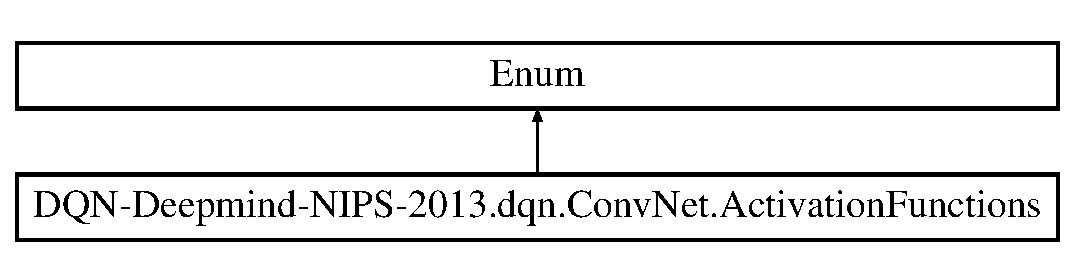
\includegraphics[height=2.000000cm]{classDQN-Deepmind-NIPS-2013_1_1dqn_1_1ConvNet_1_1ActivationFunctions}
\end{center}
\end{figure}
\subsection*{Public Member Functions}
\begin{DoxyCompactItemize}
\item 
def \hyperlink{classDQN-Deepmind-NIPS-2013_1_1dqn_1_1ConvNet_1_1ActivationFunctions_a5fc485b9d50dac40bc4db3ba6ca678cc}{is\+Valid} (e)
\begin{DoxyCompactList}\small\item\em The is\+Valid method check is the given value is a valid enumerated value. \end{DoxyCompactList}\end{DoxyCompactItemize}
\subsection*{Static Public Attributes}
\begin{DoxyCompactItemize}
\item 
\hyperlink{classDQN-Deepmind-NIPS-2013_1_1dqn_1_1ConvNet_1_1ActivationFunctions_a6fc2871aa17ddca2628226723a9116f5}{N\+O\+NE} = None
\begin{DoxyCompactList}\small\item\em Use the Identity activation function. \end{DoxyCompactList}\item 
\hyperlink{classDQN-Deepmind-NIPS-2013_1_1dqn_1_1ConvNet_1_1ActivationFunctions_a3684db68eadb8c00ed214af7bcbb2e3c}{relu} = Net.\+relu
\begin{DoxyCompactList}\small\item\em Use a Re\+LU activation function. \end{DoxyCompactList}\item 
\hyperlink{classDQN-Deepmind-NIPS-2013_1_1dqn_1_1ConvNet_1_1ActivationFunctions_a25cfb0b1f9d6d902e50f5bf77bf658a5}{softmax} = Net.\+softmax
\begin{DoxyCompactList}\small\item\em Use a softmax activation function. \end{DoxyCompactList}\end{DoxyCompactItemize}


\subsection{Detailed Description}
The \hyperlink{classDQN-Deepmind-NIPS-2013_1_1dqn_1_1ConvNet_1_1ActivationFunctions}{Activation\+Functions} class is an enumaration of valid activation funcitons. 

\subsection{Member Function Documentation}
\hypertarget{classDQN-Deepmind-NIPS-2013_1_1dqn_1_1ConvNet_1_1ActivationFunctions_a5fc485b9d50dac40bc4db3ba6ca678cc}{}\label{classDQN-Deepmind-NIPS-2013_1_1dqn_1_1ConvNet_1_1ActivationFunctions_a5fc485b9d50dac40bc4db3ba6ca678cc} 
\index{D\+Q\+N-\/\+Deepmind-\/\+N\+I\+P\+S-\/2013\+::dqn\+::\+Conv\+Net\+::\+Activation\+Functions@{D\+Q\+N-\/\+Deepmind-\/\+N\+I\+P\+S-\/2013\+::dqn\+::\+Conv\+Net\+::\+Activation\+Functions}!is\+Valid@{is\+Valid}}
\index{is\+Valid@{is\+Valid}!D\+Q\+N-\/\+Deepmind-\/\+N\+I\+P\+S-\/2013\+::dqn\+::\+Conv\+Net\+::\+Activation\+Functions@{D\+Q\+N-\/\+Deepmind-\/\+N\+I\+P\+S-\/2013\+::dqn\+::\+Conv\+Net\+::\+Activation\+Functions}}
\subsubsection{\texorpdfstring{is\+Valid()}{isValid()}}
{\footnotesize\ttfamily def D\+QN-\/Deepmind-\/N\+I\+PS-\/2013.dqn.\+Conv\+Net.\+Activation\+Functions.\+is\+Valid (\begin{DoxyParamCaption}\item[{}]{e }\end{DoxyParamCaption})}



The is\+Valid method check is the given value is a valid enumerated value. 


\begin{DoxyParams}{Parameters}
{\em e} & \+: The value to check\\
\hline
\end{DoxyParams}
\begin{DoxyReturn}{Returns}
True if the given value is a valid activation function or False otherwise 
\end{DoxyReturn}


\subsection{Member Data Documentation}
\hypertarget{classDQN-Deepmind-NIPS-2013_1_1dqn_1_1ConvNet_1_1ActivationFunctions_a6fc2871aa17ddca2628226723a9116f5}{}\label{classDQN-Deepmind-NIPS-2013_1_1dqn_1_1ConvNet_1_1ActivationFunctions_a6fc2871aa17ddca2628226723a9116f5} 
\index{D\+Q\+N-\/\+Deepmind-\/\+N\+I\+P\+S-\/2013\+::dqn\+::\+Conv\+Net\+::\+Activation\+Functions@{D\+Q\+N-\/\+Deepmind-\/\+N\+I\+P\+S-\/2013\+::dqn\+::\+Conv\+Net\+::\+Activation\+Functions}!N\+O\+NE@{N\+O\+NE}}
\index{N\+O\+NE@{N\+O\+NE}!D\+Q\+N-\/\+Deepmind-\/\+N\+I\+P\+S-\/2013\+::dqn\+::\+Conv\+Net\+::\+Activation\+Functions@{D\+Q\+N-\/\+Deepmind-\/\+N\+I\+P\+S-\/2013\+::dqn\+::\+Conv\+Net\+::\+Activation\+Functions}}
\subsubsection{\texorpdfstring{N\+O\+NE}{NONE}}
{\footnotesize\ttfamily D\+QN-\/Deepmind-\/N\+I\+PS-\/2013.dqn.\+Conv\+Net.\+Activation\+Functions.\+N\+O\+NE = None\hspace{0.3cm}{\ttfamily [static]}}



Use the Identity activation function. 

\hypertarget{classDQN-Deepmind-NIPS-2013_1_1dqn_1_1ConvNet_1_1ActivationFunctions_a3684db68eadb8c00ed214af7bcbb2e3c}{}\label{classDQN-Deepmind-NIPS-2013_1_1dqn_1_1ConvNet_1_1ActivationFunctions_a3684db68eadb8c00ed214af7bcbb2e3c} 
\index{D\+Q\+N-\/\+Deepmind-\/\+N\+I\+P\+S-\/2013\+::dqn\+::\+Conv\+Net\+::\+Activation\+Functions@{D\+Q\+N-\/\+Deepmind-\/\+N\+I\+P\+S-\/2013\+::dqn\+::\+Conv\+Net\+::\+Activation\+Functions}!relu@{relu}}
\index{relu@{relu}!D\+Q\+N-\/\+Deepmind-\/\+N\+I\+P\+S-\/2013\+::dqn\+::\+Conv\+Net\+::\+Activation\+Functions@{D\+Q\+N-\/\+Deepmind-\/\+N\+I\+P\+S-\/2013\+::dqn\+::\+Conv\+Net\+::\+Activation\+Functions}}
\subsubsection{\texorpdfstring{relu}{relu}}
{\footnotesize\ttfamily D\+QN-\/Deepmind-\/N\+I\+PS-\/2013.dqn.\+Conv\+Net.\+Activation\+Functions.\+relu = Net.\+relu\hspace{0.3cm}{\ttfamily [static]}}



Use a Re\+LU activation function. 

\hypertarget{classDQN-Deepmind-NIPS-2013_1_1dqn_1_1ConvNet_1_1ActivationFunctions_a25cfb0b1f9d6d902e50f5bf77bf658a5}{}\label{classDQN-Deepmind-NIPS-2013_1_1dqn_1_1ConvNet_1_1ActivationFunctions_a25cfb0b1f9d6d902e50f5bf77bf658a5} 
\index{D\+Q\+N-\/\+Deepmind-\/\+N\+I\+P\+S-\/2013\+::dqn\+::\+Conv\+Net\+::\+Activation\+Functions@{D\+Q\+N-\/\+Deepmind-\/\+N\+I\+P\+S-\/2013\+::dqn\+::\+Conv\+Net\+::\+Activation\+Functions}!softmax@{softmax}}
\index{softmax@{softmax}!D\+Q\+N-\/\+Deepmind-\/\+N\+I\+P\+S-\/2013\+::dqn\+::\+Conv\+Net\+::\+Activation\+Functions@{D\+Q\+N-\/\+Deepmind-\/\+N\+I\+P\+S-\/2013\+::dqn\+::\+Conv\+Net\+::\+Activation\+Functions}}
\subsubsection{\texorpdfstring{softmax}{softmax}}
{\footnotesize\ttfamily D\+QN-\/Deepmind-\/N\+I\+PS-\/2013.dqn.\+Conv\+Net.\+Activation\+Functions.\+softmax = Net.\+softmax\hspace{0.3cm}{\ttfamily [static]}}



Use a softmax activation function. 



The documentation for this class was generated from the following file\+:\begin{DoxyCompactItemize}
\item 
dqn/\hyperlink{ConvNet_8py}{Conv\+Net.\+py}\end{DoxyCompactItemize}

\hypertarget{classDQN-Deepmind-NIPS-2013_1_1agent_1_1Agent_1_1Agent}{}\section{D\+Q\+N-\/\+Deepmind-\/\+N\+I\+P\+S-\/2013.agent.\+Agent.\+Agent Class Reference}
\label{classDQN-Deepmind-NIPS-2013_1_1agent_1_1Agent_1_1Agent}\index{D\+Q\+N-\/\+Deepmind-\/\+N\+I\+P\+S-\/2013.\+agent.\+Agent.\+Agent@{D\+Q\+N-\/\+Deepmind-\/\+N\+I\+P\+S-\/2013.\+agent.\+Agent.\+Agent}}


The agent class is the base for any intelligent agent.  


Inheritance diagram for D\+Q\+N-\/\+Deepmind-\/\+N\+I\+P\+S-\/2013.agent.\+Agent.\+Agent\+:\begin{figure}[H]
\begin{center}
\leavevmode
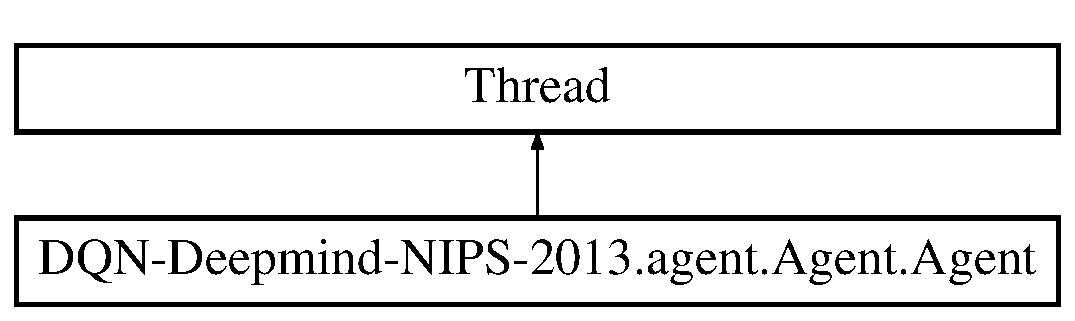
\includegraphics[height=2.000000cm]{classDQN-Deepmind-NIPS-2013_1_1agent_1_1Agent_1_1Agent}
\end{center}
\end{figure}
\subsection*{Public Member Functions}
\begin{DoxyCompactItemize}
\item 
def \hyperlink{classDQN-Deepmind-NIPS-2013_1_1agent_1_1Agent_1_1Agent_a3902963eaecb4b9dbe9bd0c06c2f9f01}{\+\_\+\+\_\+init\+\_\+\+\_\+} (self, message)
\begin{DoxyCompactList}\small\item\em \hyperlink{classDQN-Deepmind-NIPS-2013_1_1agent_1_1Agent_1_1Agent}{Agent} constructor. \end{DoxyCompactList}\item 
def \hyperlink{classDQN-Deepmind-NIPS-2013_1_1agent_1_1Agent_1_1Agent_ae41ae14645afb3279112e9d02991be99}{run} (self)
\begin{DoxyCompactList}\small\item\em The run method overrides the threading.\+Thread.\+run method. \end{DoxyCompactList}\item 
def \hyperlink{classDQN-Deepmind-NIPS-2013_1_1agent_1_1Agent_1_1Agent_a6cb1d914ca2954f968d2512f4dac3a36}{continue\+Processing} (self)
\begin{DoxyCompactList}\small\item\em The continue\+Processing return wheter the agent should continue current job or if it should stop. \end{DoxyCompactList}\item 
def \hyperlink{classDQN-Deepmind-NIPS-2013_1_1agent_1_1Agent_1_1Agent_a1662a18fd255f7c6e7a696ad4dd45304}{stop\+Processing} (self)
\begin{DoxyCompactList}\small\item\em The stop\+Processing method tells the agent to stop what it\textquotesingle{}s doing. \end{DoxyCompactList}\item 
def \hyperlink{classDQN-Deepmind-NIPS-2013_1_1agent_1_1Agent_1_1Agent_ae3b350736392d8ce39e7973d630f437a}{train} (self)
\begin{DoxyCompactList}\small\item\em The train method is an abstract method. \end{DoxyCompactList}\end{DoxyCompactItemize}


\subsection{Detailed Description}
The agent class is the base for any intelligent agent. 

\subsection{Constructor \& Destructor Documentation}
\hypertarget{classDQN-Deepmind-NIPS-2013_1_1agent_1_1Agent_1_1Agent_a3902963eaecb4b9dbe9bd0c06c2f9f01}{}\label{classDQN-Deepmind-NIPS-2013_1_1agent_1_1Agent_1_1Agent_a3902963eaecb4b9dbe9bd0c06c2f9f01} 
\index{D\+Q\+N-\/\+Deepmind-\/\+N\+I\+P\+S-\/2013\+::agent\+::\+Agent\+::\+Agent@{D\+Q\+N-\/\+Deepmind-\/\+N\+I\+P\+S-\/2013\+::agent\+::\+Agent\+::\+Agent}!\+\_\+\+\_\+init\+\_\+\+\_\+@{\+\_\+\+\_\+init\+\_\+\+\_\+}}
\index{\+\_\+\+\_\+init\+\_\+\+\_\+@{\+\_\+\+\_\+init\+\_\+\+\_\+}!D\+Q\+N-\/\+Deepmind-\/\+N\+I\+P\+S-\/2013\+::agent\+::\+Agent\+::\+Agent@{D\+Q\+N-\/\+Deepmind-\/\+N\+I\+P\+S-\/2013\+::agent\+::\+Agent\+::\+Agent}}
\subsubsection{\texorpdfstring{\+\_\+\+\_\+init\+\_\+\+\_\+()}{\_\_init\_\_()}}
{\footnotesize\ttfamily def D\+QN-\/Deepmind-\/N\+I\+PS-\/2013.agent.\+Agent.\+Agent.\+\_\+\+\_\+init\+\_\+\+\_\+ (\begin{DoxyParamCaption}\item[{}]{self,  }\item[{}]{message }\end{DoxyParamCaption})}



\hyperlink{classDQN-Deepmind-NIPS-2013_1_1agent_1_1Agent_1_1Agent}{Agent} constructor. 


\begin{DoxyParams}{Parameters}
{\em message} & \+: A message object that allows the agent to communicate with the main thread \\
\hline
\end{DoxyParams}


\subsection{Member Function Documentation}
\hypertarget{classDQN-Deepmind-NIPS-2013_1_1agent_1_1Agent_1_1Agent_a6cb1d914ca2954f968d2512f4dac3a36}{}\label{classDQN-Deepmind-NIPS-2013_1_1agent_1_1Agent_1_1Agent_a6cb1d914ca2954f968d2512f4dac3a36} 
\index{D\+Q\+N-\/\+Deepmind-\/\+N\+I\+P\+S-\/2013\+::agent\+::\+Agent\+::\+Agent@{D\+Q\+N-\/\+Deepmind-\/\+N\+I\+P\+S-\/2013\+::agent\+::\+Agent\+::\+Agent}!continue\+Processing@{continue\+Processing}}
\index{continue\+Processing@{continue\+Processing}!D\+Q\+N-\/\+Deepmind-\/\+N\+I\+P\+S-\/2013\+::agent\+::\+Agent\+::\+Agent@{D\+Q\+N-\/\+Deepmind-\/\+N\+I\+P\+S-\/2013\+::agent\+::\+Agent\+::\+Agent}}
\subsubsection{\texorpdfstring{continue\+Processing()}{continueProcessing()}}
{\footnotesize\ttfamily def D\+QN-\/Deepmind-\/N\+I\+PS-\/2013.agent.\+Agent.\+Agent.\+continue\+Processing (\begin{DoxyParamCaption}\item[{}]{self }\end{DoxyParamCaption})}



The continue\+Processing return wheter the agent should continue current job or if it should stop. 

\begin{DoxyReturn}{Returns}
True if the agent should contine, False if it should stop 
\end{DoxyReturn}
\hypertarget{classDQN-Deepmind-NIPS-2013_1_1agent_1_1Agent_1_1Agent_ae41ae14645afb3279112e9d02991be99}{}\label{classDQN-Deepmind-NIPS-2013_1_1agent_1_1Agent_1_1Agent_ae41ae14645afb3279112e9d02991be99} 
\index{D\+Q\+N-\/\+Deepmind-\/\+N\+I\+P\+S-\/2013\+::agent\+::\+Agent\+::\+Agent@{D\+Q\+N-\/\+Deepmind-\/\+N\+I\+P\+S-\/2013\+::agent\+::\+Agent\+::\+Agent}!run@{run}}
\index{run@{run}!D\+Q\+N-\/\+Deepmind-\/\+N\+I\+P\+S-\/2013\+::agent\+::\+Agent\+::\+Agent@{D\+Q\+N-\/\+Deepmind-\/\+N\+I\+P\+S-\/2013\+::agent\+::\+Agent\+::\+Agent}}
\subsubsection{\texorpdfstring{run()}{run()}}
{\footnotesize\ttfamily def D\+QN-\/Deepmind-\/N\+I\+PS-\/2013.agent.\+Agent.\+Agent.\+run (\begin{DoxyParamCaption}\item[{}]{self }\end{DoxyParamCaption})}



The run method overrides the threading.\+Thread.\+run method. 

\hypertarget{classDQN-Deepmind-NIPS-2013_1_1agent_1_1Agent_1_1Agent_a1662a18fd255f7c6e7a696ad4dd45304}{}\label{classDQN-Deepmind-NIPS-2013_1_1agent_1_1Agent_1_1Agent_a1662a18fd255f7c6e7a696ad4dd45304} 
\index{D\+Q\+N-\/\+Deepmind-\/\+N\+I\+P\+S-\/2013\+::agent\+::\+Agent\+::\+Agent@{D\+Q\+N-\/\+Deepmind-\/\+N\+I\+P\+S-\/2013\+::agent\+::\+Agent\+::\+Agent}!stop\+Processing@{stop\+Processing}}
\index{stop\+Processing@{stop\+Processing}!D\+Q\+N-\/\+Deepmind-\/\+N\+I\+P\+S-\/2013\+::agent\+::\+Agent\+::\+Agent@{D\+Q\+N-\/\+Deepmind-\/\+N\+I\+P\+S-\/2013\+::agent\+::\+Agent\+::\+Agent}}
\subsubsection{\texorpdfstring{stop\+Processing()}{stopProcessing()}}
{\footnotesize\ttfamily def D\+QN-\/Deepmind-\/N\+I\+PS-\/2013.agent.\+Agent.\+Agent.\+stop\+Processing (\begin{DoxyParamCaption}\item[{}]{self }\end{DoxyParamCaption})}



The stop\+Processing method tells the agent to stop what it\textquotesingle{}s doing. 

\hypertarget{classDQN-Deepmind-NIPS-2013_1_1agent_1_1Agent_1_1Agent_ae3b350736392d8ce39e7973d630f437a}{}\label{classDQN-Deepmind-NIPS-2013_1_1agent_1_1Agent_1_1Agent_ae3b350736392d8ce39e7973d630f437a} 
\index{D\+Q\+N-\/\+Deepmind-\/\+N\+I\+P\+S-\/2013\+::agent\+::\+Agent\+::\+Agent@{D\+Q\+N-\/\+Deepmind-\/\+N\+I\+P\+S-\/2013\+::agent\+::\+Agent\+::\+Agent}!train@{train}}
\index{train@{train}!D\+Q\+N-\/\+Deepmind-\/\+N\+I\+P\+S-\/2013\+::agent\+::\+Agent\+::\+Agent@{D\+Q\+N-\/\+Deepmind-\/\+N\+I\+P\+S-\/2013\+::agent\+::\+Agent\+::\+Agent}}
\subsubsection{\texorpdfstring{train()}{train()}}
{\footnotesize\ttfamily def D\+QN-\/Deepmind-\/N\+I\+PS-\/2013.agent.\+Agent.\+Agent.\+train (\begin{DoxyParamCaption}\item[{}]{self }\end{DoxyParamCaption})}



The train method is an abstract method. 

An actual agent should override this method with one that trains the agent and loop until stop\+Processing is called by the main thread 

The documentation for this class was generated from the following file\+:\begin{DoxyCompactItemize}
\item 
agent/\hyperlink{Agent_8py}{Agent.\+py}\end{DoxyCompactItemize}

\hypertarget{classDQN-Deepmind-NIPS-2013_1_1EnvDisplay_1_1Canvas}{}\section{D\+Q\+N-\/\+Deepmind-\/\+N\+I\+P\+S-\/2013.Env\+Display.\+Canvas Class Reference}
\label{classDQN-Deepmind-NIPS-2013_1_1EnvDisplay_1_1Canvas}\index{D\+Q\+N-\/\+Deepmind-\/\+N\+I\+P\+S-\/2013.\+Env\+Display.\+Canvas@{D\+Q\+N-\/\+Deepmind-\/\+N\+I\+P\+S-\/2013.\+Env\+Display.\+Canvas}}


The \hyperlink{classDQN-Deepmind-NIPS-2013_1_1EnvDisplay_1_1Canvas}{Canvas} class is a Qt\+Gui.\+Q\+Widget that display an image.  


Inheritance diagram for D\+Q\+N-\/\+Deepmind-\/\+N\+I\+P\+S-\/2013.Env\+Display.\+Canvas\+:\begin{figure}[H]
\begin{center}
\leavevmode
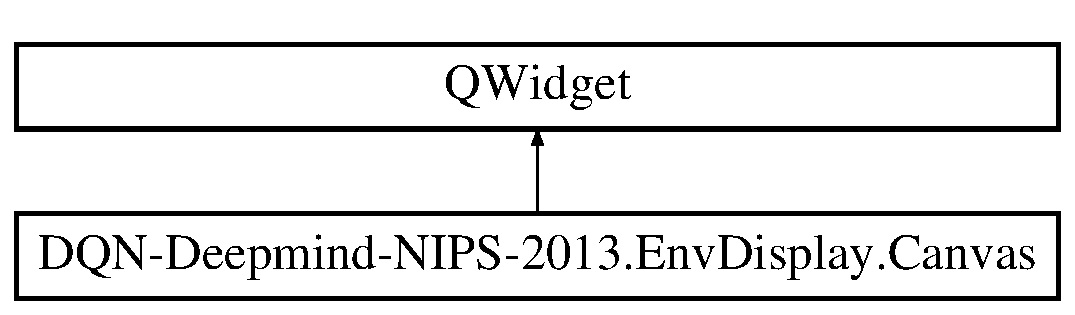
\includegraphics[height=2.000000cm]{classDQN-Deepmind-NIPS-2013_1_1EnvDisplay_1_1Canvas}
\end{center}
\end{figure}
\subsection*{Public Member Functions}
\begin{DoxyCompactItemize}
\item 
def \hyperlink{classDQN-Deepmind-NIPS-2013_1_1EnvDisplay_1_1Canvas_ae4988f04f58e179d82925dd7b6157ee7}{\+\_\+\+\_\+init\+\_\+\+\_\+} (self, env)
\begin{DoxyCompactList}\small\item\em The \hyperlink{classDQN-Deepmind-NIPS-2013_1_1EnvDisplay_1_1Canvas}{Canvas} class constructor. \end{DoxyCompactList}\item 
def \hyperlink{classDQN-Deepmind-NIPS-2013_1_1EnvDisplay_1_1Canvas_a6225ff0fed4f12c11640877f04286c91}{draw\+Screen} (self)
\begin{DoxyCompactList}\small\item\em The draw\+Screen methods order the \hyperlink{classDQN-Deepmind-NIPS-2013_1_1EnvDisplay_1_1Canvas}{Canvas} object to update the image to display with the current screen from the game environment. \end{DoxyCompactList}\item 
def \hyperlink{classDQN-Deepmind-NIPS-2013_1_1EnvDisplay_1_1Canvas_a7bb5fe211a49f4ead25e6ebdb02f32af}{paint\+Event} (self, event)
\begin{DoxyCompactList}\small\item\em The paint\+Event method overrides the Qt\+Gui.\+Q\+Widget method and simply repaint the current image. \end{DoxyCompactList}\end{DoxyCompactItemize}


\subsection{Detailed Description}
The \hyperlink{classDQN-Deepmind-NIPS-2013_1_1EnvDisplay_1_1Canvas}{Canvas} class is a Qt\+Gui.\+Q\+Widget that display an image. 

\subsection{Constructor \& Destructor Documentation}
\hypertarget{classDQN-Deepmind-NIPS-2013_1_1EnvDisplay_1_1Canvas_ae4988f04f58e179d82925dd7b6157ee7}{}\label{classDQN-Deepmind-NIPS-2013_1_1EnvDisplay_1_1Canvas_ae4988f04f58e179d82925dd7b6157ee7} 
\index{D\+Q\+N-\/\+Deepmind-\/\+N\+I\+P\+S-\/2013\+::\+Env\+Display\+::\+Canvas@{D\+Q\+N-\/\+Deepmind-\/\+N\+I\+P\+S-\/2013\+::\+Env\+Display\+::\+Canvas}!\+\_\+\+\_\+init\+\_\+\+\_\+@{\+\_\+\+\_\+init\+\_\+\+\_\+}}
\index{\+\_\+\+\_\+init\+\_\+\+\_\+@{\+\_\+\+\_\+init\+\_\+\+\_\+}!D\+Q\+N-\/\+Deepmind-\/\+N\+I\+P\+S-\/2013\+::\+Env\+Display\+::\+Canvas@{D\+Q\+N-\/\+Deepmind-\/\+N\+I\+P\+S-\/2013\+::\+Env\+Display\+::\+Canvas}}
\subsubsection{\texorpdfstring{\+\_\+\+\_\+init\+\_\+\+\_\+()}{\_\_init\_\_()}}
{\footnotesize\ttfamily def D\+QN-\/Deepmind-\/N\+I\+PS-\/2013.Env\+Display.\+Canvas.\+\_\+\+\_\+init\+\_\+\+\_\+ (\begin{DoxyParamCaption}\item[{}]{self,  }\item[{}]{env }\end{DoxyParamCaption})}



The \hyperlink{classDQN-Deepmind-NIPS-2013_1_1EnvDisplay_1_1Canvas}{Canvas} class constructor. 


\begin{DoxyParams}{Parameters}
{\em env} & \+: The \hyperlink{namespaceDQN-Deepmind-NIPS-2013_1_1GameEnv}{Game\+Env} object to use to retrieve the game screen \\
\hline
\end{DoxyParams}


\subsection{Member Function Documentation}
\hypertarget{classDQN-Deepmind-NIPS-2013_1_1EnvDisplay_1_1Canvas_a6225ff0fed4f12c11640877f04286c91}{}\label{classDQN-Deepmind-NIPS-2013_1_1EnvDisplay_1_1Canvas_a6225ff0fed4f12c11640877f04286c91} 
\index{D\+Q\+N-\/\+Deepmind-\/\+N\+I\+P\+S-\/2013\+::\+Env\+Display\+::\+Canvas@{D\+Q\+N-\/\+Deepmind-\/\+N\+I\+P\+S-\/2013\+::\+Env\+Display\+::\+Canvas}!draw\+Screen@{draw\+Screen}}
\index{draw\+Screen@{draw\+Screen}!D\+Q\+N-\/\+Deepmind-\/\+N\+I\+P\+S-\/2013\+::\+Env\+Display\+::\+Canvas@{D\+Q\+N-\/\+Deepmind-\/\+N\+I\+P\+S-\/2013\+::\+Env\+Display\+::\+Canvas}}
\subsubsection{\texorpdfstring{draw\+Screen()}{drawScreen()}}
{\footnotesize\ttfamily def D\+QN-\/Deepmind-\/N\+I\+PS-\/2013.Env\+Display.\+Canvas.\+draw\+Screen (\begin{DoxyParamCaption}\item[{}]{self }\end{DoxyParamCaption})}



The draw\+Screen methods order the \hyperlink{classDQN-Deepmind-NIPS-2013_1_1EnvDisplay_1_1Canvas}{Canvas} object to update the image to display with the current screen from the game environment. 

\hypertarget{classDQN-Deepmind-NIPS-2013_1_1EnvDisplay_1_1Canvas_a7bb5fe211a49f4ead25e6ebdb02f32af}{}\label{classDQN-Deepmind-NIPS-2013_1_1EnvDisplay_1_1Canvas_a7bb5fe211a49f4ead25e6ebdb02f32af} 
\index{D\+Q\+N-\/\+Deepmind-\/\+N\+I\+P\+S-\/2013\+::\+Env\+Display\+::\+Canvas@{D\+Q\+N-\/\+Deepmind-\/\+N\+I\+P\+S-\/2013\+::\+Env\+Display\+::\+Canvas}!paint\+Event@{paint\+Event}}
\index{paint\+Event@{paint\+Event}!D\+Q\+N-\/\+Deepmind-\/\+N\+I\+P\+S-\/2013\+::\+Env\+Display\+::\+Canvas@{D\+Q\+N-\/\+Deepmind-\/\+N\+I\+P\+S-\/2013\+::\+Env\+Display\+::\+Canvas}}
\subsubsection{\texorpdfstring{paint\+Event()}{paintEvent()}}
{\footnotesize\ttfamily def D\+QN-\/Deepmind-\/N\+I\+PS-\/2013.Env\+Display.\+Canvas.\+paint\+Event (\begin{DoxyParamCaption}\item[{}]{self,  }\item[{}]{event }\end{DoxyParamCaption})}



The paint\+Event method overrides the Qt\+Gui.\+Q\+Widget method and simply repaint the current image. 


\begin{DoxyParams}{Parameters}
{\em event} & \\
\hline
\end{DoxyParams}


The documentation for this class was generated from the following file\+:\begin{DoxyCompactItemize}
\item 
\hyperlink{EnvDisplay_8py}{Env\+Display.\+py}\end{DoxyCompactItemize}

\hypertarget{classDQN-Deepmind-NIPS-2013_1_1agent_1_1DeepMindAgent_1_1DeepMindAgent}{}\section{D\+Q\+N-\/\+Deepmind-\/\+N\+I\+P\+S-\/2013.agent.\+Deep\+Mind\+Agent.\+Deep\+Mind\+Agent Class Reference}
\label{classDQN-Deepmind-NIPS-2013_1_1agent_1_1DeepMindAgent_1_1DeepMindAgent}\index{D\+Q\+N-\/\+Deepmind-\/\+N\+I\+P\+S-\/2013.\+agent.\+Deep\+Mind\+Agent.\+Deep\+Mind\+Agent@{D\+Q\+N-\/\+Deepmind-\/\+N\+I\+P\+S-\/2013.\+agent.\+Deep\+Mind\+Agent.\+Deep\+Mind\+Agent}}


The \hyperlink{classDQN-Deepmind-NIPS-2013_1_1agent_1_1DeepMindAgent_1_1DeepMindAgent}{Deep\+Mind\+Agent} class implements the agent described by Deepmind in their article of 2013 \char`\"{}\+Playing Atari with Deep Reinforcement Learning\char`\"{}.  


Inheritance diagram for D\+Q\+N-\/\+Deepmind-\/\+N\+I\+P\+S-\/2013.agent.\+Deep\+Mind\+Agent.\+Deep\+Mind\+Agent\+:\begin{figure}[H]
\begin{center}
\leavevmode
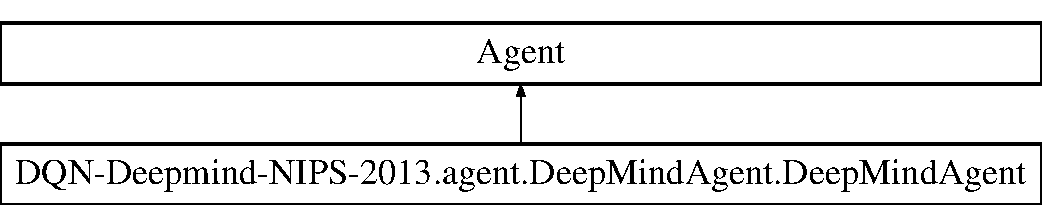
\includegraphics[height=2.000000cm]{classDQN-Deepmind-NIPS-2013_1_1agent_1_1DeepMindAgent_1_1DeepMindAgent}
\end{center}
\end{figure}
\subsection*{Public Member Functions}
\begin{DoxyCompactItemize}
\item 
def \hyperlink{classDQN-Deepmind-NIPS-2013_1_1agent_1_1DeepMindAgent_1_1DeepMindAgent_a9ea279d64a3b2bced6901c55df78c7e4}{create\+New\+Agent} (message, saver, plotter, env, name)
\begin{DoxyCompactList}\small\item\em The create\+New\+Agent static method returns a new agent with the given name. \end{DoxyCompactList}\item 
def \hyperlink{classDQN-Deepmind-NIPS-2013_1_1agent_1_1DeepMindAgent_1_1DeepMindAgent_a6271c469fb0446dd92a94ce447ba3695}{load\+Agent} (message, saver, plotter, env, agent\+Id)
\begin{DoxyCompactList}\small\item\em The load\+Agent static method returns an agent build from a previously saved agent using the last network saved by this agent. \end{DoxyCompactList}\item 
def \hyperlink{classDQN-Deepmind-NIPS-2013_1_1agent_1_1DeepMindAgent_1_1DeepMindAgent_a8bbe0f1127879b400142d5cf6fea5384}{\+\_\+\+\_\+init\+\_\+\+\_\+} (self, message, saver, plotter, env, agent\+Id)
\begin{DoxyCompactList}\small\item\em The agent agent constructor. \end{DoxyCompactList}\item 
def \hyperlink{classDQN-Deepmind-NIPS-2013_1_1agent_1_1DeepMindAgent_1_1DeepMindAgent_ae3b30ec9438fbaa91c440415e43844fe}{load\+Params} (self)
\begin{DoxyCompactList}\small\item\em The load\+Params object load the parameters of the current agent saved in the saver object. \end{DoxyCompactList}\item 
def \hyperlink{classDQN-Deepmind-NIPS-2013_1_1agent_1_1DeepMindAgent_1_1DeepMindAgent_a63ce7439d1d1989c262489e08e04e204}{load\+Network} (self, network\+Id)
\begin{DoxyCompactList}\small\item\em The load\+Network object load the network associated with the given id. \end{DoxyCompactList}\end{DoxyCompactItemize}
\subsection*{Public Attributes}
\begin{DoxyCompactItemize}
\item 
\hyperlink{classDQN-Deepmind-NIPS-2013_1_1agent_1_1DeepMindAgent_1_1DeepMindAgent_a63e93b51f5b355b0896957d4484a8fb3}{id}
\begin{DoxyCompactList}\small\item\em The id of the agent as used in the saver. \end{DoxyCompactList}\end{DoxyCompactItemize}


\subsection{Detailed Description}
The \hyperlink{classDQN-Deepmind-NIPS-2013_1_1agent_1_1DeepMindAgent_1_1DeepMindAgent}{Deep\+Mind\+Agent} class implements the agent described by Deepmind in their article of 2013 \char`\"{}\+Playing Atari with Deep Reinforcement Learning\char`\"{}. 

\begin{DoxySeeAlso}{See also}
$<$a href\char`\"{}https\+://arxiv.\+org/abs/1312.\+5602\char`\"{}$>$Playing Atari with Deep Reinforcement Learning 
\end{DoxySeeAlso}


\subsection{Constructor \& Destructor Documentation}
\hypertarget{classDQN-Deepmind-NIPS-2013_1_1agent_1_1DeepMindAgent_1_1DeepMindAgent_a8bbe0f1127879b400142d5cf6fea5384}{}\label{classDQN-Deepmind-NIPS-2013_1_1agent_1_1DeepMindAgent_1_1DeepMindAgent_a8bbe0f1127879b400142d5cf6fea5384} 
\index{D\+Q\+N-\/\+Deepmind-\/\+N\+I\+P\+S-\/2013\+::agent\+::\+Deep\+Mind\+Agent\+::\+Deep\+Mind\+Agent@{D\+Q\+N-\/\+Deepmind-\/\+N\+I\+P\+S-\/2013\+::agent\+::\+Deep\+Mind\+Agent\+::\+Deep\+Mind\+Agent}!\+\_\+\+\_\+init\+\_\+\+\_\+@{\+\_\+\+\_\+init\+\_\+\+\_\+}}
\index{\+\_\+\+\_\+init\+\_\+\+\_\+@{\+\_\+\+\_\+init\+\_\+\+\_\+}!D\+Q\+N-\/\+Deepmind-\/\+N\+I\+P\+S-\/2013\+::agent\+::\+Deep\+Mind\+Agent\+::\+Deep\+Mind\+Agent@{D\+Q\+N-\/\+Deepmind-\/\+N\+I\+P\+S-\/2013\+::agent\+::\+Deep\+Mind\+Agent\+::\+Deep\+Mind\+Agent}}
\subsubsection{\texorpdfstring{\+\_\+\+\_\+init\+\_\+\+\_\+()}{\_\_init\_\_()}}
{\footnotesize\ttfamily def D\+QN-\/Deepmind-\/N\+I\+PS-\/2013.agent.\+Deep\+Mind\+Agent.\+Deep\+Mind\+Agent.\+\_\+\+\_\+init\+\_\+\+\_\+ (\begin{DoxyParamCaption}\item[{}]{self,  }\item[{}]{message,  }\item[{}]{saver,  }\item[{}]{plotter,  }\item[{}]{env,  }\item[{}]{agent\+Id }\end{DoxyParamCaption})}



The agent agent constructor. 

This shouldn\textquotesingle{}t be directly called. Instread, the static methods create\+New\+Agent or load\+Agent should be used


\begin{DoxyParams}{Parameters}
{\em message} & \+: The message object that the agent uses to communicate whith the main thread \\
\hline
{\em saver} & \+: The saver object that the agent uses to save itself \\
\hline
{\em plotter} & \+: The plotter object the agent can use to plot some datas \\
\hline
{\em env} & \+: The game\+Environement the agent will use as input \\
\hline
{\em agent\+Id} & \+: The id of the agent \\
\hline
\end{DoxyParams}


\subsection{Member Function Documentation}
\hypertarget{classDQN-Deepmind-NIPS-2013_1_1agent_1_1DeepMindAgent_1_1DeepMindAgent_a9ea279d64a3b2bced6901c55df78c7e4}{}\label{classDQN-Deepmind-NIPS-2013_1_1agent_1_1DeepMindAgent_1_1DeepMindAgent_a9ea279d64a3b2bced6901c55df78c7e4} 
\index{D\+Q\+N-\/\+Deepmind-\/\+N\+I\+P\+S-\/2013\+::agent\+::\+Deep\+Mind\+Agent\+::\+Deep\+Mind\+Agent@{D\+Q\+N-\/\+Deepmind-\/\+N\+I\+P\+S-\/2013\+::agent\+::\+Deep\+Mind\+Agent\+::\+Deep\+Mind\+Agent}!create\+New\+Agent@{create\+New\+Agent}}
\index{create\+New\+Agent@{create\+New\+Agent}!D\+Q\+N-\/\+Deepmind-\/\+N\+I\+P\+S-\/2013\+::agent\+::\+Deep\+Mind\+Agent\+::\+Deep\+Mind\+Agent@{D\+Q\+N-\/\+Deepmind-\/\+N\+I\+P\+S-\/2013\+::agent\+::\+Deep\+Mind\+Agent\+::\+Deep\+Mind\+Agent}}
\subsubsection{\texorpdfstring{create\+New\+Agent()}{createNewAgent()}}
{\footnotesize\ttfamily def D\+QN-\/Deepmind-\/N\+I\+PS-\/2013.agent.\+Deep\+Mind\+Agent.\+Deep\+Mind\+Agent.\+create\+New\+Agent (\begin{DoxyParamCaption}\item[{}]{message,  }\item[{}]{saver,  }\item[{}]{plotter,  }\item[{}]{env,  }\item[{}]{name }\end{DoxyParamCaption})}



The create\+New\+Agent static method returns a new agent with the given name. 


\begin{DoxyParams}{Parameters}
{\em message} & \+: The message object that the agent uses to communicate whith the main thread \\
\hline
{\em saver} & \+: The saver object that the agent uses to save itself \\
\hline
{\em plotter} & \+: The plotter object the agent can use to plot some datas \\
\hline
{\em env} & \+: The game\+Environement the agent will use as input \\
\hline
{\em name} & \+: The name of the agent\\
\hline
\end{DoxyParams}
\begin{DoxyReturn}{Returns}
A new agent that\textquotesingle{}s saved in the saver object 
\end{DoxyReturn}
\hypertarget{classDQN-Deepmind-NIPS-2013_1_1agent_1_1DeepMindAgent_1_1DeepMindAgent_a6271c469fb0446dd92a94ce447ba3695}{}\label{classDQN-Deepmind-NIPS-2013_1_1agent_1_1DeepMindAgent_1_1DeepMindAgent_a6271c469fb0446dd92a94ce447ba3695} 
\index{D\+Q\+N-\/\+Deepmind-\/\+N\+I\+P\+S-\/2013\+::agent\+::\+Deep\+Mind\+Agent\+::\+Deep\+Mind\+Agent@{D\+Q\+N-\/\+Deepmind-\/\+N\+I\+P\+S-\/2013\+::agent\+::\+Deep\+Mind\+Agent\+::\+Deep\+Mind\+Agent}!load\+Agent@{load\+Agent}}
\index{load\+Agent@{load\+Agent}!D\+Q\+N-\/\+Deepmind-\/\+N\+I\+P\+S-\/2013\+::agent\+::\+Deep\+Mind\+Agent\+::\+Deep\+Mind\+Agent@{D\+Q\+N-\/\+Deepmind-\/\+N\+I\+P\+S-\/2013\+::agent\+::\+Deep\+Mind\+Agent\+::\+Deep\+Mind\+Agent}}
\subsubsection{\texorpdfstring{load\+Agent()}{loadAgent()}}
{\footnotesize\ttfamily def D\+QN-\/Deepmind-\/N\+I\+PS-\/2013.agent.\+Deep\+Mind\+Agent.\+Deep\+Mind\+Agent.\+load\+Agent (\begin{DoxyParamCaption}\item[{}]{message,  }\item[{}]{saver,  }\item[{}]{plotter,  }\item[{}]{env,  }\item[{}]{agent\+Id }\end{DoxyParamCaption})}



The load\+Agent static method returns an agent build from a previously saved agent using the last network saved by this agent. 


\begin{DoxyParams}{Parameters}
{\em message} & \+: The message object that the agent uses to communicate whith the main thread \\
\hline
{\em saver} & \+: The saver object that the agent uses to save itself \\
\hline
{\em plotter} & \+: The plotter object the agent can use to plot some datas \\
\hline
{\em env} & \+: The game\+Environement the agent will use as input \\
\hline
{\em agent\+Id} & \+: The id of the agent to copy\\
\hline
\end{DoxyParams}
\begin{DoxyReturn}{Returns}
A new agent initilized with the datas previously stored in the saver object 
\end{DoxyReturn}
\hypertarget{classDQN-Deepmind-NIPS-2013_1_1agent_1_1DeepMindAgent_1_1DeepMindAgent_a63ce7439d1d1989c262489e08e04e204}{}\label{classDQN-Deepmind-NIPS-2013_1_1agent_1_1DeepMindAgent_1_1DeepMindAgent_a63ce7439d1d1989c262489e08e04e204} 
\index{D\+Q\+N-\/\+Deepmind-\/\+N\+I\+P\+S-\/2013\+::agent\+::\+Deep\+Mind\+Agent\+::\+Deep\+Mind\+Agent@{D\+Q\+N-\/\+Deepmind-\/\+N\+I\+P\+S-\/2013\+::agent\+::\+Deep\+Mind\+Agent\+::\+Deep\+Mind\+Agent}!load\+Network@{load\+Network}}
\index{load\+Network@{load\+Network}!D\+Q\+N-\/\+Deepmind-\/\+N\+I\+P\+S-\/2013\+::agent\+::\+Deep\+Mind\+Agent\+::\+Deep\+Mind\+Agent@{D\+Q\+N-\/\+Deepmind-\/\+N\+I\+P\+S-\/2013\+::agent\+::\+Deep\+Mind\+Agent\+::\+Deep\+Mind\+Agent}}
\subsubsection{\texorpdfstring{load\+Network()}{loadNetwork()}}
{\footnotesize\ttfamily def D\+QN-\/Deepmind-\/N\+I\+PS-\/2013.agent.\+Deep\+Mind\+Agent.\+Deep\+Mind\+Agent.\+load\+Network (\begin{DoxyParamCaption}\item[{}]{self,  }\item[{}]{network\+Id }\end{DoxyParamCaption})}



The load\+Network object load the network associated with the given id. 


\begin{DoxyParams}{Parameters}
{\em network\+Id} & \+: The id of the network to load \\
\hline
\end{DoxyParams}
\hypertarget{classDQN-Deepmind-NIPS-2013_1_1agent_1_1DeepMindAgent_1_1DeepMindAgent_ae3b30ec9438fbaa91c440415e43844fe}{}\label{classDQN-Deepmind-NIPS-2013_1_1agent_1_1DeepMindAgent_1_1DeepMindAgent_ae3b30ec9438fbaa91c440415e43844fe} 
\index{D\+Q\+N-\/\+Deepmind-\/\+N\+I\+P\+S-\/2013\+::agent\+::\+Deep\+Mind\+Agent\+::\+Deep\+Mind\+Agent@{D\+Q\+N-\/\+Deepmind-\/\+N\+I\+P\+S-\/2013\+::agent\+::\+Deep\+Mind\+Agent\+::\+Deep\+Mind\+Agent}!load\+Params@{load\+Params}}
\index{load\+Params@{load\+Params}!D\+Q\+N-\/\+Deepmind-\/\+N\+I\+P\+S-\/2013\+::agent\+::\+Deep\+Mind\+Agent\+::\+Deep\+Mind\+Agent@{D\+Q\+N-\/\+Deepmind-\/\+N\+I\+P\+S-\/2013\+::agent\+::\+Deep\+Mind\+Agent\+::\+Deep\+Mind\+Agent}}
\subsubsection{\texorpdfstring{load\+Params()}{loadParams()}}
{\footnotesize\ttfamily def D\+QN-\/Deepmind-\/N\+I\+PS-\/2013.agent.\+Deep\+Mind\+Agent.\+Deep\+Mind\+Agent.\+load\+Params (\begin{DoxyParamCaption}\item[{}]{self }\end{DoxyParamCaption})}



The load\+Params object load the parameters of the current agent saved in the saver object. 



\subsection{Member Data Documentation}
\hypertarget{classDQN-Deepmind-NIPS-2013_1_1agent_1_1DeepMindAgent_1_1DeepMindAgent_a63e93b51f5b355b0896957d4484a8fb3}{}\label{classDQN-Deepmind-NIPS-2013_1_1agent_1_1DeepMindAgent_1_1DeepMindAgent_a63e93b51f5b355b0896957d4484a8fb3} 
\index{D\+Q\+N-\/\+Deepmind-\/\+N\+I\+P\+S-\/2013\+::agent\+::\+Deep\+Mind\+Agent\+::\+Deep\+Mind\+Agent@{D\+Q\+N-\/\+Deepmind-\/\+N\+I\+P\+S-\/2013\+::agent\+::\+Deep\+Mind\+Agent\+::\+Deep\+Mind\+Agent}!id@{id}}
\index{id@{id}!D\+Q\+N-\/\+Deepmind-\/\+N\+I\+P\+S-\/2013\+::agent\+::\+Deep\+Mind\+Agent\+::\+Deep\+Mind\+Agent@{D\+Q\+N-\/\+Deepmind-\/\+N\+I\+P\+S-\/2013\+::agent\+::\+Deep\+Mind\+Agent\+::\+Deep\+Mind\+Agent}}
\subsubsection{\texorpdfstring{id}{id}}
{\footnotesize\ttfamily D\+QN-\/Deepmind-\/N\+I\+PS-\/2013.agent.\+Deep\+Mind\+Agent.\+Deep\+Mind\+Agent.\+id}



The id of the agent as used in the saver. 



The documentation for this class was generated from the following file\+:\begin{DoxyCompactItemize}
\item 
agent/\hyperlink{DeepMindAgent_8py}{Deep\+Mind\+Agent.\+py}\end{DoxyCompactItemize}

\hypertarget{classDQN-Deepmind-NIPS-2013_1_1QtDisplay_1_1DisplayHandler}{}\section{D\+Q\+N-\/\+Deepmind-\/\+N\+I\+P\+S-\/2013.Qt\+Display.\+Display\+Handler Class Reference}
\label{classDQN-Deepmind-NIPS-2013_1_1QtDisplay_1_1DisplayHandler}\index{D\+Q\+N-\/\+Deepmind-\/\+N\+I\+P\+S-\/2013.\+Qt\+Display.\+Display\+Handler@{D\+Q\+N-\/\+Deepmind-\/\+N\+I\+P\+S-\/2013.\+Qt\+Display.\+Display\+Handler}}


The \hyperlink{classDQN-Deepmind-NIPS-2013_1_1QtDisplay_1_1DisplayHandler}{Display\+Handler} class implements a thread that will be responsible of managing any windows or other display or Qt events.  


Inheritance diagram for D\+Q\+N-\/\+Deepmind-\/\+N\+I\+P\+S-\/2013.Qt\+Display.\+Display\+Handler\+:\begin{figure}[H]
\begin{center}
\leavevmode
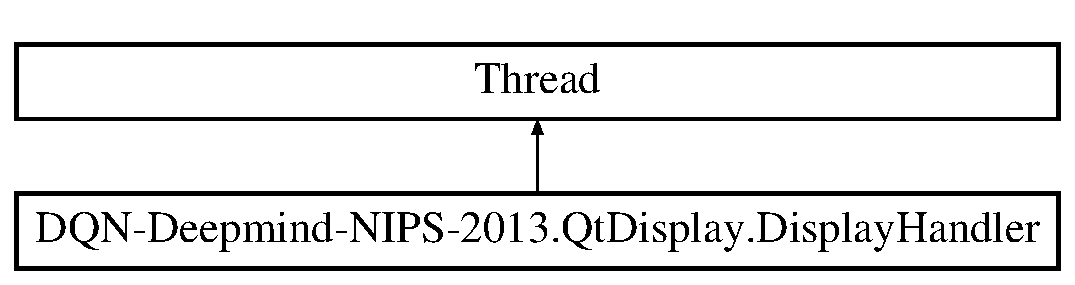
\includegraphics[height=2.000000cm]{classDQN-Deepmind-NIPS-2013_1_1QtDisplay_1_1DisplayHandler}
\end{center}
\end{figure}
\subsection*{Public Member Functions}
\begin{DoxyCompactItemize}
\item 
def \hyperlink{classDQN-Deepmind-NIPS-2013_1_1QtDisplay_1_1DisplayHandler_a417807e1b454c0cc3e86a8bddb2e6aee}{\+\_\+\+\_\+init\+\_\+\+\_\+} (self)
\begin{DoxyCompactList}\small\item\em The \hyperlink{classDQN-Deepmind-NIPS-2013_1_1QtDisplay_1_1DisplayHandler}{Display\+Handler} constructor initialize the thread. \end{DoxyCompactList}\item 
def \hyperlink{classDQN-Deepmind-NIPS-2013_1_1QtDisplay_1_1DisplayHandler_a1f995b71cfad970a33d358737a90970a}{run} (self)
\begin{DoxyCompactList}\small\item\em The run method initilizes the Qt display and start the event loop. \end{DoxyCompactList}\item 
def \hyperlink{classDQN-Deepmind-NIPS-2013_1_1QtDisplay_1_1DisplayHandler_a1c18d34e62cbeff7c6d75a8eeb02506b}{Qt} (self)
\begin{DoxyCompactList}\small\item\em The Qt methods wait for the Qt display to be reday and returns it. \end{DoxyCompactList}\item 
def \hyperlink{classDQN-Deepmind-NIPS-2013_1_1QtDisplay_1_1DisplayHandler_a9f10007a3cf4bfdf8b3908f57ef03b7b}{exit} (self)
\begin{DoxyCompactList}\small\item\em The exit method force the \hyperlink{classDQN-Deepmind-NIPS-2013_1_1QtDisplay_1_1QDisplay}{Q\+Display} object to leave its event loop and wait for the current thread to terminate. \end{DoxyCompactList}\end{DoxyCompactItemize}
\subsection*{Public Attributes}
\begin{DoxyCompactItemize}
\item 
\hyperlink{classDQN-Deepmind-NIPS-2013_1_1QtDisplay_1_1DisplayHandler_a5c3b4122e47a768cd3ef67f478ee25c0}{qt\+\_\+ready}
\begin{DoxyCompactList}\small\item\em An event that indicates all the signals are connected. \end{DoxyCompactList}\end{DoxyCompactItemize}


\subsection{Detailed Description}
The \hyperlink{classDQN-Deepmind-NIPS-2013_1_1QtDisplay_1_1DisplayHandler}{Display\+Handler} class implements a thread that will be responsible of managing any windows or other display or Qt events. 

\subsection{Constructor \& Destructor Documentation}
\hypertarget{classDQN-Deepmind-NIPS-2013_1_1QtDisplay_1_1DisplayHandler_a417807e1b454c0cc3e86a8bddb2e6aee}{}\label{classDQN-Deepmind-NIPS-2013_1_1QtDisplay_1_1DisplayHandler_a417807e1b454c0cc3e86a8bddb2e6aee} 
\index{D\+Q\+N-\/\+Deepmind-\/\+N\+I\+P\+S-\/2013\+::\+Qt\+Display\+::\+Display\+Handler@{D\+Q\+N-\/\+Deepmind-\/\+N\+I\+P\+S-\/2013\+::\+Qt\+Display\+::\+Display\+Handler}!\+\_\+\+\_\+init\+\_\+\+\_\+@{\+\_\+\+\_\+init\+\_\+\+\_\+}}
\index{\+\_\+\+\_\+init\+\_\+\+\_\+@{\+\_\+\+\_\+init\+\_\+\+\_\+}!D\+Q\+N-\/\+Deepmind-\/\+N\+I\+P\+S-\/2013\+::\+Qt\+Display\+::\+Display\+Handler@{D\+Q\+N-\/\+Deepmind-\/\+N\+I\+P\+S-\/2013\+::\+Qt\+Display\+::\+Display\+Handler}}
\subsubsection{\texorpdfstring{\+\_\+\+\_\+init\+\_\+\+\_\+()}{\_\_init\_\_()}}
{\footnotesize\ttfamily def D\+QN-\/Deepmind-\/N\+I\+PS-\/2013.Qt\+Display.\+Display\+Handler.\+\_\+\+\_\+init\+\_\+\+\_\+ (\begin{DoxyParamCaption}\item[{}]{self }\end{DoxyParamCaption})}



The \hyperlink{classDQN-Deepmind-NIPS-2013_1_1QtDisplay_1_1DisplayHandler}{Display\+Handler} constructor initialize the thread. 



\subsection{Member Function Documentation}
\hypertarget{classDQN-Deepmind-NIPS-2013_1_1QtDisplay_1_1DisplayHandler_a9f10007a3cf4bfdf8b3908f57ef03b7b}{}\label{classDQN-Deepmind-NIPS-2013_1_1QtDisplay_1_1DisplayHandler_a9f10007a3cf4bfdf8b3908f57ef03b7b} 
\index{D\+Q\+N-\/\+Deepmind-\/\+N\+I\+P\+S-\/2013\+::\+Qt\+Display\+::\+Display\+Handler@{D\+Q\+N-\/\+Deepmind-\/\+N\+I\+P\+S-\/2013\+::\+Qt\+Display\+::\+Display\+Handler}!exit@{exit}}
\index{exit@{exit}!D\+Q\+N-\/\+Deepmind-\/\+N\+I\+P\+S-\/2013\+::\+Qt\+Display\+::\+Display\+Handler@{D\+Q\+N-\/\+Deepmind-\/\+N\+I\+P\+S-\/2013\+::\+Qt\+Display\+::\+Display\+Handler}}
\subsubsection{\texorpdfstring{exit()}{exit()}}
{\footnotesize\ttfamily def D\+QN-\/Deepmind-\/N\+I\+PS-\/2013.Qt\+Display.\+Display\+Handler.\+exit (\begin{DoxyParamCaption}\item[{}]{self }\end{DoxyParamCaption})}



The exit method force the \hyperlink{classDQN-Deepmind-NIPS-2013_1_1QtDisplay_1_1QDisplay}{Q\+Display} object to leave its event loop and wait for the current thread to terminate. 

\hypertarget{classDQN-Deepmind-NIPS-2013_1_1QtDisplay_1_1DisplayHandler_a1c18d34e62cbeff7c6d75a8eeb02506b}{}\label{classDQN-Deepmind-NIPS-2013_1_1QtDisplay_1_1DisplayHandler_a1c18d34e62cbeff7c6d75a8eeb02506b} 
\index{D\+Q\+N-\/\+Deepmind-\/\+N\+I\+P\+S-\/2013\+::\+Qt\+Display\+::\+Display\+Handler@{D\+Q\+N-\/\+Deepmind-\/\+N\+I\+P\+S-\/2013\+::\+Qt\+Display\+::\+Display\+Handler}!Qt@{Qt}}
\index{Qt@{Qt}!D\+Q\+N-\/\+Deepmind-\/\+N\+I\+P\+S-\/2013\+::\+Qt\+Display\+::\+Display\+Handler@{D\+Q\+N-\/\+Deepmind-\/\+N\+I\+P\+S-\/2013\+::\+Qt\+Display\+::\+Display\+Handler}}
\subsubsection{\texorpdfstring{Qt()}{Qt()}}
{\footnotesize\ttfamily def D\+QN-\/Deepmind-\/N\+I\+PS-\/2013.Qt\+Display.\+Display\+Handler.\+Qt (\begin{DoxyParamCaption}\item[{}]{self }\end{DoxyParamCaption})}



The Qt methods wait for the Qt display to be reday and returns it. 

\begin{DoxyReturn}{Returns}
A reference to the \hyperlink{classDQN-Deepmind-NIPS-2013_1_1QtDisplay_1_1QDisplay}{Q\+Display} object managed by this thread 
\end{DoxyReturn}
\hypertarget{classDQN-Deepmind-NIPS-2013_1_1QtDisplay_1_1DisplayHandler_a1f995b71cfad970a33d358737a90970a}{}\label{classDQN-Deepmind-NIPS-2013_1_1QtDisplay_1_1DisplayHandler_a1f995b71cfad970a33d358737a90970a} 
\index{D\+Q\+N-\/\+Deepmind-\/\+N\+I\+P\+S-\/2013\+::\+Qt\+Display\+::\+Display\+Handler@{D\+Q\+N-\/\+Deepmind-\/\+N\+I\+P\+S-\/2013\+::\+Qt\+Display\+::\+Display\+Handler}!run@{run}}
\index{run@{run}!D\+Q\+N-\/\+Deepmind-\/\+N\+I\+P\+S-\/2013\+::\+Qt\+Display\+::\+Display\+Handler@{D\+Q\+N-\/\+Deepmind-\/\+N\+I\+P\+S-\/2013\+::\+Qt\+Display\+::\+Display\+Handler}}
\subsubsection{\texorpdfstring{run()}{run()}}
{\footnotesize\ttfamily def D\+QN-\/Deepmind-\/N\+I\+PS-\/2013.Qt\+Display.\+Display\+Handler.\+run (\begin{DoxyParamCaption}\item[{}]{self }\end{DoxyParamCaption})}



The run method initilizes the Qt display and start the event loop. 



\subsection{Member Data Documentation}
\hypertarget{classDQN-Deepmind-NIPS-2013_1_1QtDisplay_1_1DisplayHandler_a5c3b4122e47a768cd3ef67f478ee25c0}{}\label{classDQN-Deepmind-NIPS-2013_1_1QtDisplay_1_1DisplayHandler_a5c3b4122e47a768cd3ef67f478ee25c0} 
\index{D\+Q\+N-\/\+Deepmind-\/\+N\+I\+P\+S-\/2013\+::\+Qt\+Display\+::\+Display\+Handler@{D\+Q\+N-\/\+Deepmind-\/\+N\+I\+P\+S-\/2013\+::\+Qt\+Display\+::\+Display\+Handler}!qt\+\_\+ready@{qt\+\_\+ready}}
\index{qt\+\_\+ready@{qt\+\_\+ready}!D\+Q\+N-\/\+Deepmind-\/\+N\+I\+P\+S-\/2013\+::\+Qt\+Display\+::\+Display\+Handler@{D\+Q\+N-\/\+Deepmind-\/\+N\+I\+P\+S-\/2013\+::\+Qt\+Display\+::\+Display\+Handler}}
\subsubsection{\texorpdfstring{qt\+\_\+ready}{qt\_ready}}
{\footnotesize\ttfamily D\+QN-\/Deepmind-\/N\+I\+PS-\/2013.Qt\+Display.\+Display\+Handler.\+qt\+\_\+ready}



An event that indicates all the signals are connected. 



The documentation for this class was generated from the following file\+:\begin{DoxyCompactItemize}
\item 
\hyperlink{QtDisplay_8py}{Qt\+Display.\+py}\end{DoxyCompactItemize}

\hypertarget{classDQN-Deepmind-NIPS-2013_1_1EnvDisplay_1_1EnvDisplay}{}\section{D\+Q\+N-\/\+Deepmind-\/\+N\+I\+P\+S-\/2013.Env\+Display.\+Env\+Display Class Reference}
\label{classDQN-Deepmind-NIPS-2013_1_1EnvDisplay_1_1EnvDisplay}\index{D\+Q\+N-\/\+Deepmind-\/\+N\+I\+P\+S-\/2013.\+Env\+Display.\+Env\+Display@{D\+Q\+N-\/\+Deepmind-\/\+N\+I\+P\+S-\/2013.\+Env\+Display.\+Env\+Display}}


The \hyperlink{classDQN-Deepmind-NIPS-2013_1_1EnvDisplay_1_1EnvDisplay}{Env\+Display} class is responsible of displaying and periodically refresh the display of the game environment.  


Inheritance diagram for D\+Q\+N-\/\+Deepmind-\/\+N\+I\+P\+S-\/2013.Env\+Display.\+Env\+Display\+:\begin{figure}[H]
\begin{center}
\leavevmode
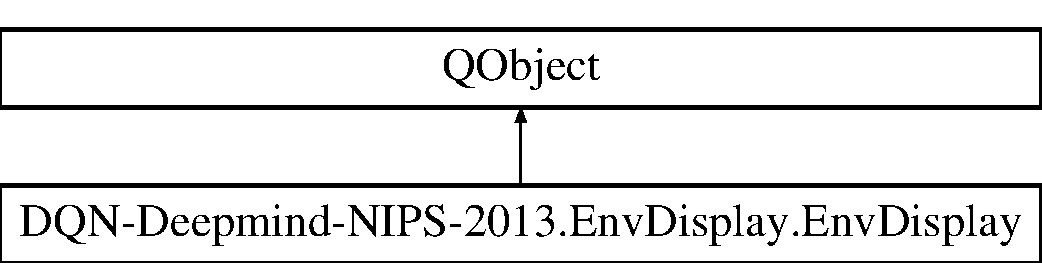
\includegraphics[height=2.000000cm]{classDQN-Deepmind-NIPS-2013_1_1EnvDisplay_1_1EnvDisplay}
\end{center}
\end{figure}
\subsection*{Public Member Functions}
\begin{DoxyCompactItemize}
\item 
def \hyperlink{classDQN-Deepmind-NIPS-2013_1_1EnvDisplay_1_1EnvDisplay_ad60e1788026fe76998cc85b558d9311f}{\+\_\+\+\_\+init\+\_\+\+\_\+} (self, env, freq=30)
\begin{DoxyCompactList}\small\item\em The \hyperlink{classDQN-Deepmind-NIPS-2013_1_1EnvDisplay_1_1EnvDisplay}{Env\+Display} constructor. \end{DoxyCompactList}\end{DoxyCompactItemize}


\subsection{Detailed Description}
The \hyperlink{classDQN-Deepmind-NIPS-2013_1_1EnvDisplay_1_1EnvDisplay}{Env\+Display} class is responsible of displaying and periodically refresh the display of the game environment. 

\subsection{Constructor \& Destructor Documentation}
\hypertarget{classDQN-Deepmind-NIPS-2013_1_1EnvDisplay_1_1EnvDisplay_ad60e1788026fe76998cc85b558d9311f}{}\label{classDQN-Deepmind-NIPS-2013_1_1EnvDisplay_1_1EnvDisplay_ad60e1788026fe76998cc85b558d9311f} 
\index{D\+Q\+N-\/\+Deepmind-\/\+N\+I\+P\+S-\/2013\+::\+Env\+Display\+::\+Env\+Display@{D\+Q\+N-\/\+Deepmind-\/\+N\+I\+P\+S-\/2013\+::\+Env\+Display\+::\+Env\+Display}!\+\_\+\+\_\+init\+\_\+\+\_\+@{\+\_\+\+\_\+init\+\_\+\+\_\+}}
\index{\+\_\+\+\_\+init\+\_\+\+\_\+@{\+\_\+\+\_\+init\+\_\+\+\_\+}!D\+Q\+N-\/\+Deepmind-\/\+N\+I\+P\+S-\/2013\+::\+Env\+Display\+::\+Env\+Display@{D\+Q\+N-\/\+Deepmind-\/\+N\+I\+P\+S-\/2013\+::\+Env\+Display\+::\+Env\+Display}}
\subsubsection{\texorpdfstring{\+\_\+\+\_\+init\+\_\+\+\_\+()}{\_\_init\_\_()}}
{\footnotesize\ttfamily def D\+QN-\/Deepmind-\/N\+I\+PS-\/2013.Env\+Display.\+Env\+Display.\+\_\+\+\_\+init\+\_\+\+\_\+ (\begin{DoxyParamCaption}\item[{}]{self,  }\item[{}]{env,  }\item[{}]{freq = {\ttfamily 30} }\end{DoxyParamCaption})}



The \hyperlink{classDQN-Deepmind-NIPS-2013_1_1EnvDisplay_1_1EnvDisplay}{Env\+Display} constructor. 


\begin{DoxyParams}{Parameters}
{\em env} & \+: the \hyperlink{namespaceDQN-Deepmind-NIPS-2013_1_1GameEnv}{Game\+Env} object to use \\
\hline
{\em freq} & \+: refresh rate \\
\hline
\end{DoxyParams}


The documentation for this class was generated from the following file\+:\begin{DoxyCompactItemize}
\item 
\hyperlink{EnvDisplay_8py}{Env\+Display.\+py}\end{DoxyCompactItemize}

\hypertarget{classDQN-Deepmind-NIPS-2013_1_1GameEnv_1_1GameEnv}{}\section{D\+Q\+N-\/\+Deepmind-\/\+N\+I\+P\+S-\/2013.Game\+Env.\+Game\+Env Class Reference}
\label{classDQN-Deepmind-NIPS-2013_1_1GameEnv_1_1GameEnv}\index{D\+Q\+N-\/\+Deepmind-\/\+N\+I\+P\+S-\/2013.\+Game\+Env.\+Game\+Env@{D\+Q\+N-\/\+Deepmind-\/\+N\+I\+P\+S-\/2013.\+Game\+Env.\+Game\+Env}}


The \hyperlink{classDQN-Deepmind-NIPS-2013_1_1GameEnv_1_1GameEnv}{Game\+Env} class provides a way for the agent to interact with the game.  


\subsection*{Public Member Functions}
\begin{DoxyCompactItemize}
\item 
def \hyperlink{classDQN-Deepmind-NIPS-2013_1_1GameEnv_1_1GameEnv_a787af9d0e467c038e970246ae4dfdc08}{\+\_\+\+\_\+init\+\_\+\+\_\+} (self, rom, \hyperlink{classDQN-Deepmind-NIPS-2013_1_1GameEnv_1_1GameEnv_ae8e7e56bd996ea0ce4ece1ca32f6b54a}{out\+Size})
\begin{DoxyCompactList}\small\item\em The \hyperlink{classDQN-Deepmind-NIPS-2013_1_1GameEnv_1_1GameEnv}{Game\+Env} constructor. \end{DoxyCompactList}\item 
def \hyperlink{classDQN-Deepmind-NIPS-2013_1_1GameEnv_1_1GameEnv_a76014d9140e479757a52b9ceda06dd16}{min\+Actions} (self)
\begin{DoxyCompactList}\small\item\em The min\+Actions method retuns an array containing the minimal action set for the loaded game. \end{DoxyCompactList}\item 
def \hyperlink{classDQN-Deepmind-NIPS-2013_1_1GameEnv_1_1GameEnv_ab2efa70a8316abde73936602001654a6}{leg\+Actions} (self)
\begin{DoxyCompactList}\small\item\em The leg\+Actions method returns an array containing the set of legal actions. \end{DoxyCompactList}\item 
def \hyperlink{classDQN-Deepmind-NIPS-2013_1_1GameEnv_1_1GameEnv_a37712548267b91afddb6866fddf22b94}{get\+Screen} (self)
\begin{DoxyCompactList}\small\item\em The get\+Screen method converts the game screen to a grayscale array shrink it to the configured size and returns it. \end{DoxyCompactList}\item 
def \hyperlink{classDQN-Deepmind-NIPS-2013_1_1GameEnv_1_1GameEnv_a553c6eac3cac494bff5c9703dcfea2fe}{get\+Screen\+R\+GB} (self)
\begin{DoxyCompactList}\small\item\em The get\+Screen\+R\+GB method returns an array containing the R\+BG screen. \end{DoxyCompactList}\item 
def \hyperlink{classDQN-Deepmind-NIPS-2013_1_1GameEnv_1_1GameEnv_a675bec246ea3ed4506328deb5df64d4e}{act} (self, action)
\begin{DoxyCompactList}\small\item\em The act method performs the given action and returns the reward gained from that action. \end{DoxyCompactList}\item 
def \hyperlink{classDQN-Deepmind-NIPS-2013_1_1GameEnv_1_1GameEnv_afc780b83378b9d19d9dba64711e5c2ed}{reset\+Game} (self)
\begin{DoxyCompactList}\small\item\em The reset\+Game method reset the game. \end{DoxyCompactList}\item 
def \hyperlink{classDQN-Deepmind-NIPS-2013_1_1GameEnv_1_1GameEnv_a1ccc35e029e05910c3c25ffa602e442b}{game\+Over} (self)
\begin{DoxyCompactList}\small\item\em The game\+Over methods return whether or not the game ended. \end{DoxyCompactList}\end{DoxyCompactItemize}
\subsection*{Public Attributes}
\begin{DoxyCompactItemize}
\item 
\hyperlink{classDQN-Deepmind-NIPS-2013_1_1GameEnv_1_1GameEnv_a2dedb2f4e5f0f1b7da2970ac89a5b544}{screen\+Size}
\begin{DoxyCompactList}\small\item\em The size of the screen in the form \mbox{[}height, width\mbox{]}. \end{DoxyCompactList}\item 
\hyperlink{classDQN-Deepmind-NIPS-2013_1_1GameEnv_1_1GameEnv_ae8e7e56bd996ea0ce4ece1ca32f6b54a}{out\+Size}
\begin{DoxyCompactList}\small\item\em The size of the images returned by get\+Screen the form \mbox{[}height, width\mbox{]}. \end{DoxyCompactList}\end{DoxyCompactItemize}


\subsection{Detailed Description}
The \hyperlink{classDQN-Deepmind-NIPS-2013_1_1GameEnv_1_1GameEnv}{Game\+Env} class provides a way for the agent to interact with the game. 

\subsection{Constructor \& Destructor Documentation}
\hypertarget{classDQN-Deepmind-NIPS-2013_1_1GameEnv_1_1GameEnv_a787af9d0e467c038e970246ae4dfdc08}{}\label{classDQN-Deepmind-NIPS-2013_1_1GameEnv_1_1GameEnv_a787af9d0e467c038e970246ae4dfdc08} 
\index{D\+Q\+N-\/\+Deepmind-\/\+N\+I\+P\+S-\/2013\+::\+Game\+Env\+::\+Game\+Env@{D\+Q\+N-\/\+Deepmind-\/\+N\+I\+P\+S-\/2013\+::\+Game\+Env\+::\+Game\+Env}!\+\_\+\+\_\+init\+\_\+\+\_\+@{\+\_\+\+\_\+init\+\_\+\+\_\+}}
\index{\+\_\+\+\_\+init\+\_\+\+\_\+@{\+\_\+\+\_\+init\+\_\+\+\_\+}!D\+Q\+N-\/\+Deepmind-\/\+N\+I\+P\+S-\/2013\+::\+Game\+Env\+::\+Game\+Env@{D\+Q\+N-\/\+Deepmind-\/\+N\+I\+P\+S-\/2013\+::\+Game\+Env\+::\+Game\+Env}}
\subsubsection{\texorpdfstring{\+\_\+\+\_\+init\+\_\+\+\_\+()}{\_\_init\_\_()}}
{\footnotesize\ttfamily def D\+QN-\/Deepmind-\/N\+I\+PS-\/2013.Game\+Env.\+Game\+Env.\+\_\+\+\_\+init\+\_\+\+\_\+ (\begin{DoxyParamCaption}\item[{}]{self,  }\item[{}]{rom,  }\item[{}]{out\+Size }\end{DoxyParamCaption})}



The \hyperlink{classDQN-Deepmind-NIPS-2013_1_1GameEnv_1_1GameEnv}{Game\+Env} constructor. 


\begin{DoxyParams}{Parameters}
{\em rom} & \+: The path to the rom to load \\
\hline
{\em out\+Size} & \+: An array of two elements \mbox{[}h, w\mbox{]} where h is the height of the image to output with the method get\+Screen and w its width \\
\hline
\end{DoxyParams}


\subsection{Member Function Documentation}
\hypertarget{classDQN-Deepmind-NIPS-2013_1_1GameEnv_1_1GameEnv_a675bec246ea3ed4506328deb5df64d4e}{}\label{classDQN-Deepmind-NIPS-2013_1_1GameEnv_1_1GameEnv_a675bec246ea3ed4506328deb5df64d4e} 
\index{D\+Q\+N-\/\+Deepmind-\/\+N\+I\+P\+S-\/2013\+::\+Game\+Env\+::\+Game\+Env@{D\+Q\+N-\/\+Deepmind-\/\+N\+I\+P\+S-\/2013\+::\+Game\+Env\+::\+Game\+Env}!act@{act}}
\index{act@{act}!D\+Q\+N-\/\+Deepmind-\/\+N\+I\+P\+S-\/2013\+::\+Game\+Env\+::\+Game\+Env@{D\+Q\+N-\/\+Deepmind-\/\+N\+I\+P\+S-\/2013\+::\+Game\+Env\+::\+Game\+Env}}
\subsubsection{\texorpdfstring{act()}{act()}}
{\footnotesize\ttfamily def D\+QN-\/Deepmind-\/N\+I\+PS-\/2013.Game\+Env.\+Game\+Env.\+act (\begin{DoxyParamCaption}\item[{}]{self,  }\item[{}]{action }\end{DoxyParamCaption})}



The act method performs the given action and returns the reward gained from that action. 

\begin{DoxyReturn}{Returns}
The reward issued from the action taken 
\end{DoxyReturn}
\hypertarget{classDQN-Deepmind-NIPS-2013_1_1GameEnv_1_1GameEnv_a1ccc35e029e05910c3c25ffa602e442b}{}\label{classDQN-Deepmind-NIPS-2013_1_1GameEnv_1_1GameEnv_a1ccc35e029e05910c3c25ffa602e442b} 
\index{D\+Q\+N-\/\+Deepmind-\/\+N\+I\+P\+S-\/2013\+::\+Game\+Env\+::\+Game\+Env@{D\+Q\+N-\/\+Deepmind-\/\+N\+I\+P\+S-\/2013\+::\+Game\+Env\+::\+Game\+Env}!game\+Over@{game\+Over}}
\index{game\+Over@{game\+Over}!D\+Q\+N-\/\+Deepmind-\/\+N\+I\+P\+S-\/2013\+::\+Game\+Env\+::\+Game\+Env@{D\+Q\+N-\/\+Deepmind-\/\+N\+I\+P\+S-\/2013\+::\+Game\+Env\+::\+Game\+Env}}
\subsubsection{\texorpdfstring{game\+Over()}{gameOver()}}
{\footnotesize\ttfamily def D\+QN-\/Deepmind-\/N\+I\+PS-\/2013.Game\+Env.\+Game\+Env.\+game\+Over (\begin{DoxyParamCaption}\item[{}]{self }\end{DoxyParamCaption})}



The game\+Over methods return whether or not the game ended. 

\begin{DoxyReturn}{Returns}
True if the game is in an terminal state, False otherwise 
\end{DoxyReturn}
\hypertarget{classDQN-Deepmind-NIPS-2013_1_1GameEnv_1_1GameEnv_a37712548267b91afddb6866fddf22b94}{}\label{classDQN-Deepmind-NIPS-2013_1_1GameEnv_1_1GameEnv_a37712548267b91afddb6866fddf22b94} 
\index{D\+Q\+N-\/\+Deepmind-\/\+N\+I\+P\+S-\/2013\+::\+Game\+Env\+::\+Game\+Env@{D\+Q\+N-\/\+Deepmind-\/\+N\+I\+P\+S-\/2013\+::\+Game\+Env\+::\+Game\+Env}!get\+Screen@{get\+Screen}}
\index{get\+Screen@{get\+Screen}!D\+Q\+N-\/\+Deepmind-\/\+N\+I\+P\+S-\/2013\+::\+Game\+Env\+::\+Game\+Env@{D\+Q\+N-\/\+Deepmind-\/\+N\+I\+P\+S-\/2013\+::\+Game\+Env\+::\+Game\+Env}}
\subsubsection{\texorpdfstring{get\+Screen()}{getScreen()}}
{\footnotesize\ttfamily def D\+QN-\/Deepmind-\/N\+I\+PS-\/2013.Game\+Env.\+Game\+Env.\+get\+Screen (\begin{DoxyParamCaption}\item[{}]{self }\end{DoxyParamCaption})}



The get\+Screen method converts the game screen to a grayscale array shrink it to the configured size and returns it. 

\begin{DoxyReturn}{Returns}
A numpy array of numpy.\+float32 between 0 and 255 and of shape \hyperlink{classDQN-Deepmind-NIPS-2013_1_1GameEnv_1_1GameEnv_ae8e7e56bd996ea0ce4ece1ca32f6b54a}{Game\+Env.\+out\+Size} 
\end{DoxyReturn}
\hypertarget{classDQN-Deepmind-NIPS-2013_1_1GameEnv_1_1GameEnv_a553c6eac3cac494bff5c9703dcfea2fe}{}\label{classDQN-Deepmind-NIPS-2013_1_1GameEnv_1_1GameEnv_a553c6eac3cac494bff5c9703dcfea2fe} 
\index{D\+Q\+N-\/\+Deepmind-\/\+N\+I\+P\+S-\/2013\+::\+Game\+Env\+::\+Game\+Env@{D\+Q\+N-\/\+Deepmind-\/\+N\+I\+P\+S-\/2013\+::\+Game\+Env\+::\+Game\+Env}!get\+Screen\+R\+GB@{get\+Screen\+R\+GB}}
\index{get\+Screen\+R\+GB@{get\+Screen\+R\+GB}!D\+Q\+N-\/\+Deepmind-\/\+N\+I\+P\+S-\/2013\+::\+Game\+Env\+::\+Game\+Env@{D\+Q\+N-\/\+Deepmind-\/\+N\+I\+P\+S-\/2013\+::\+Game\+Env\+::\+Game\+Env}}
\subsubsection{\texorpdfstring{get\+Screen\+R\+G\+B()}{getScreenRGB()}}
{\footnotesize\ttfamily def D\+QN-\/Deepmind-\/N\+I\+PS-\/2013.Game\+Env.\+Game\+Env.\+get\+Screen\+R\+GB (\begin{DoxyParamCaption}\item[{}]{self }\end{DoxyParamCaption})}



The get\+Screen\+R\+GB method returns an array containing the R\+BG screen. 

\begin{DoxyReturn}{Returns}
A numpy array of numpy.\+uint8 of shape \mbox{[}\hyperlink{classDQN-Deepmind-NIPS-2013_1_1GameEnv_1_1GameEnv_a2dedb2f4e5f0f1b7da2970ac89a5b544}{Game\+Env.\+screen\+Size}\mbox{[}0\mbox{]}, \hyperlink{classDQN-Deepmind-NIPS-2013_1_1GameEnv_1_1GameEnv_a2dedb2f4e5f0f1b7da2970ac89a5b544}{Game\+Env.\+screen\+Size}\mbox{[}1\mbox{]}, 3\mbox{]} 
\end{DoxyReturn}
\hypertarget{classDQN-Deepmind-NIPS-2013_1_1GameEnv_1_1GameEnv_ab2efa70a8316abde73936602001654a6}{}\label{classDQN-Deepmind-NIPS-2013_1_1GameEnv_1_1GameEnv_ab2efa70a8316abde73936602001654a6} 
\index{D\+Q\+N-\/\+Deepmind-\/\+N\+I\+P\+S-\/2013\+::\+Game\+Env\+::\+Game\+Env@{D\+Q\+N-\/\+Deepmind-\/\+N\+I\+P\+S-\/2013\+::\+Game\+Env\+::\+Game\+Env}!leg\+Actions@{leg\+Actions}}
\index{leg\+Actions@{leg\+Actions}!D\+Q\+N-\/\+Deepmind-\/\+N\+I\+P\+S-\/2013\+::\+Game\+Env\+::\+Game\+Env@{D\+Q\+N-\/\+Deepmind-\/\+N\+I\+P\+S-\/2013\+::\+Game\+Env\+::\+Game\+Env}}
\subsubsection{\texorpdfstring{leg\+Actions()}{legActions()}}
{\footnotesize\ttfamily def D\+QN-\/Deepmind-\/N\+I\+PS-\/2013.Game\+Env.\+Game\+Env.\+leg\+Actions (\begin{DoxyParamCaption}\item[{}]{self }\end{DoxyParamCaption})}



The leg\+Actions method returns an array containing the set of legal actions. 

\begin{DoxyReturn}{Returns}
An array containing the set of legal actions 
\end{DoxyReturn}
\hypertarget{classDQN-Deepmind-NIPS-2013_1_1GameEnv_1_1GameEnv_a76014d9140e479757a52b9ceda06dd16}{}\label{classDQN-Deepmind-NIPS-2013_1_1GameEnv_1_1GameEnv_a76014d9140e479757a52b9ceda06dd16} 
\index{D\+Q\+N-\/\+Deepmind-\/\+N\+I\+P\+S-\/2013\+::\+Game\+Env\+::\+Game\+Env@{D\+Q\+N-\/\+Deepmind-\/\+N\+I\+P\+S-\/2013\+::\+Game\+Env\+::\+Game\+Env}!min\+Actions@{min\+Actions}}
\index{min\+Actions@{min\+Actions}!D\+Q\+N-\/\+Deepmind-\/\+N\+I\+P\+S-\/2013\+::\+Game\+Env\+::\+Game\+Env@{D\+Q\+N-\/\+Deepmind-\/\+N\+I\+P\+S-\/2013\+::\+Game\+Env\+::\+Game\+Env}}
\subsubsection{\texorpdfstring{min\+Actions()}{minActions()}}
{\footnotesize\ttfamily def D\+QN-\/Deepmind-\/N\+I\+PS-\/2013.Game\+Env.\+Game\+Env.\+min\+Actions (\begin{DoxyParamCaption}\item[{}]{self }\end{DoxyParamCaption})}



The min\+Actions method retuns an array containing the minimal action set for the loaded game. 

\begin{DoxyReturn}{Returns}
An array containing the minimum set of legal actions 
\end{DoxyReturn}
\hypertarget{classDQN-Deepmind-NIPS-2013_1_1GameEnv_1_1GameEnv_afc780b83378b9d19d9dba64711e5c2ed}{}\label{classDQN-Deepmind-NIPS-2013_1_1GameEnv_1_1GameEnv_afc780b83378b9d19d9dba64711e5c2ed} 
\index{D\+Q\+N-\/\+Deepmind-\/\+N\+I\+P\+S-\/2013\+::\+Game\+Env\+::\+Game\+Env@{D\+Q\+N-\/\+Deepmind-\/\+N\+I\+P\+S-\/2013\+::\+Game\+Env\+::\+Game\+Env}!reset\+Game@{reset\+Game}}
\index{reset\+Game@{reset\+Game}!D\+Q\+N-\/\+Deepmind-\/\+N\+I\+P\+S-\/2013\+::\+Game\+Env\+::\+Game\+Env@{D\+Q\+N-\/\+Deepmind-\/\+N\+I\+P\+S-\/2013\+::\+Game\+Env\+::\+Game\+Env}}
\subsubsection{\texorpdfstring{reset\+Game()}{resetGame()}}
{\footnotesize\ttfamily def D\+QN-\/Deepmind-\/N\+I\+PS-\/2013.Game\+Env.\+Game\+Env.\+reset\+Game (\begin{DoxyParamCaption}\item[{}]{self }\end{DoxyParamCaption})}



The reset\+Game method reset the game. 



\subsection{Member Data Documentation}
\hypertarget{classDQN-Deepmind-NIPS-2013_1_1GameEnv_1_1GameEnv_ae8e7e56bd996ea0ce4ece1ca32f6b54a}{}\label{classDQN-Deepmind-NIPS-2013_1_1GameEnv_1_1GameEnv_ae8e7e56bd996ea0ce4ece1ca32f6b54a} 
\index{D\+Q\+N-\/\+Deepmind-\/\+N\+I\+P\+S-\/2013\+::\+Game\+Env\+::\+Game\+Env@{D\+Q\+N-\/\+Deepmind-\/\+N\+I\+P\+S-\/2013\+::\+Game\+Env\+::\+Game\+Env}!out\+Size@{out\+Size}}
\index{out\+Size@{out\+Size}!D\+Q\+N-\/\+Deepmind-\/\+N\+I\+P\+S-\/2013\+::\+Game\+Env\+::\+Game\+Env@{D\+Q\+N-\/\+Deepmind-\/\+N\+I\+P\+S-\/2013\+::\+Game\+Env\+::\+Game\+Env}}
\subsubsection{\texorpdfstring{out\+Size}{outSize}}
{\footnotesize\ttfamily D\+QN-\/Deepmind-\/N\+I\+PS-\/2013.Game\+Env.\+Game\+Env.\+out\+Size}



The size of the images returned by get\+Screen the form \mbox{[}height, width\mbox{]}. 

\hypertarget{classDQN-Deepmind-NIPS-2013_1_1GameEnv_1_1GameEnv_a2dedb2f4e5f0f1b7da2970ac89a5b544}{}\label{classDQN-Deepmind-NIPS-2013_1_1GameEnv_1_1GameEnv_a2dedb2f4e5f0f1b7da2970ac89a5b544} 
\index{D\+Q\+N-\/\+Deepmind-\/\+N\+I\+P\+S-\/2013\+::\+Game\+Env\+::\+Game\+Env@{D\+Q\+N-\/\+Deepmind-\/\+N\+I\+P\+S-\/2013\+::\+Game\+Env\+::\+Game\+Env}!screen\+Size@{screen\+Size}}
\index{screen\+Size@{screen\+Size}!D\+Q\+N-\/\+Deepmind-\/\+N\+I\+P\+S-\/2013\+::\+Game\+Env\+::\+Game\+Env@{D\+Q\+N-\/\+Deepmind-\/\+N\+I\+P\+S-\/2013\+::\+Game\+Env\+::\+Game\+Env}}
\subsubsection{\texorpdfstring{screen\+Size}{screenSize}}
{\footnotesize\ttfamily D\+QN-\/Deepmind-\/N\+I\+PS-\/2013.Game\+Env.\+Game\+Env.\+screen\+Size}



The size of the screen in the form \mbox{[}height, width\mbox{]}. 



The documentation for this class was generated from the following file\+:\begin{DoxyCompactItemize}
\item 
\hyperlink{GameEnv_8py}{Game\+Env.\+py}\end{DoxyCompactItemize}

\hypertarget{classDQN-Deepmind-NIPS-2013_1_1agent_1_1DeepMindAgent_1_1ImagesSet}{}\section{D\+Q\+N-\/\+Deepmind-\/\+N\+I\+P\+S-\/2013.agent.\+Deep\+Mind\+Agent.\+Images\+Set Class Reference}
\label{classDQN-Deepmind-NIPS-2013_1_1agent_1_1DeepMindAgent_1_1ImagesSet}\index{D\+Q\+N-\/\+Deepmind-\/\+N\+I\+P\+S-\/2013.\+agent.\+Deep\+Mind\+Agent.\+Images\+Set@{D\+Q\+N-\/\+Deepmind-\/\+N\+I\+P\+S-\/2013.\+agent.\+Deep\+Mind\+Agent.\+Images\+Set}}


The Image\+Set class implement an image container.  


\subsection*{Public Member Functions}
\begin{DoxyCompactItemize}
\item 
def \hyperlink{classDQN-Deepmind-NIPS-2013_1_1agent_1_1DeepMindAgent_1_1ImagesSet_ad08d7c16326d59f705dfe03ebf28120d}{\+\_\+\+\_\+init\+\_\+\+\_\+} (self, chunk\+Size, h, w)
\begin{DoxyCompactList}\small\item\em The Image\+Set constructor. \end{DoxyCompactList}\item 
def \hyperlink{classDQN-Deepmind-NIPS-2013_1_1agent_1_1DeepMindAgent_1_1ImagesSet_a27898f9b6851b1e27e34be9842859c7f}{add\+Images} (self, img\+List)
\begin{DoxyCompactList}\small\item\em The add\+Images method adds the given images to the set. \end{DoxyCompactList}\item 
def \hyperlink{classDQN-Deepmind-NIPS-2013_1_1agent_1_1DeepMindAgent_1_1ImagesSet_a044f2ad869a3ff4cf61a7e6eeccc502c}{image} (self, slot)
\begin{DoxyCompactList}\small\item\em The image method returns the image stored at the given slot. \end{DoxyCompactList}\item 
def \hyperlink{classDQN-Deepmind-NIPS-2013_1_1agent_1_1DeepMindAgent_1_1ImagesSet_a5f0032044a746fce8cdcccedc8059b57}{free} (self, slots)
\begin{DoxyCompactList}\small\item\em The free method free the given slots. \end{DoxyCompactList}\end{DoxyCompactItemize}


\subsection{Detailed Description}
The Image\+Set class implement an image container. 

The Image\+Set class expects that the images to store are numpy arrays of np.\+float32 of shape \mbox{[}h, w\mbox{]} where h is the height of the image and w its width.

If the set if full, this class pre-\/allocate an array of N images before storing new images.

The images stored in the set are actually copied 

\subsection{Constructor \& Destructor Documentation}
\hypertarget{classDQN-Deepmind-NIPS-2013_1_1agent_1_1DeepMindAgent_1_1ImagesSet_ad08d7c16326d59f705dfe03ebf28120d}{}\label{classDQN-Deepmind-NIPS-2013_1_1agent_1_1DeepMindAgent_1_1ImagesSet_ad08d7c16326d59f705dfe03ebf28120d} 
\index{D\+Q\+N-\/\+Deepmind-\/\+N\+I\+P\+S-\/2013\+::agent\+::\+Deep\+Mind\+Agent\+::\+Images\+Set@{D\+Q\+N-\/\+Deepmind-\/\+N\+I\+P\+S-\/2013\+::agent\+::\+Deep\+Mind\+Agent\+::\+Images\+Set}!\+\_\+\+\_\+init\+\_\+\+\_\+@{\+\_\+\+\_\+init\+\_\+\+\_\+}}
\index{\+\_\+\+\_\+init\+\_\+\+\_\+@{\+\_\+\+\_\+init\+\_\+\+\_\+}!D\+Q\+N-\/\+Deepmind-\/\+N\+I\+P\+S-\/2013\+::agent\+::\+Deep\+Mind\+Agent\+::\+Images\+Set@{D\+Q\+N-\/\+Deepmind-\/\+N\+I\+P\+S-\/2013\+::agent\+::\+Deep\+Mind\+Agent\+::\+Images\+Set}}
\subsubsection{\texorpdfstring{\+\_\+\+\_\+init\+\_\+\+\_\+()}{\_\_init\_\_()}}
{\footnotesize\ttfamily def D\+QN-\/Deepmind-\/N\+I\+PS-\/2013.agent.\+Deep\+Mind\+Agent.\+Images\+Set.\+\_\+\+\_\+init\+\_\+\+\_\+ (\begin{DoxyParamCaption}\item[{}]{self,  }\item[{}]{chunk\+Size,  }\item[{}]{h,  }\item[{}]{w }\end{DoxyParamCaption})}



The Image\+Set constructor. 


\begin{DoxyParams}{Parameters}
{\em chunk\+Size} & \+: The size by witch the set well be increased every time it\textquotesingle{}s full and images are inserted \\
\hline
{\em h} & \+: The images\textquotesingle{} height \\
\hline
{\em w} & \+: The images\textquotesingle{} width \\
\hline
\end{DoxyParams}


\subsection{Member Function Documentation}
\hypertarget{classDQN-Deepmind-NIPS-2013_1_1agent_1_1DeepMindAgent_1_1ImagesSet_a27898f9b6851b1e27e34be9842859c7f}{}\label{classDQN-Deepmind-NIPS-2013_1_1agent_1_1DeepMindAgent_1_1ImagesSet_a27898f9b6851b1e27e34be9842859c7f} 
\index{D\+Q\+N-\/\+Deepmind-\/\+N\+I\+P\+S-\/2013\+::agent\+::\+Deep\+Mind\+Agent\+::\+Images\+Set@{D\+Q\+N-\/\+Deepmind-\/\+N\+I\+P\+S-\/2013\+::agent\+::\+Deep\+Mind\+Agent\+::\+Images\+Set}!add\+Images@{add\+Images}}
\index{add\+Images@{add\+Images}!D\+Q\+N-\/\+Deepmind-\/\+N\+I\+P\+S-\/2013\+::agent\+::\+Deep\+Mind\+Agent\+::\+Images\+Set@{D\+Q\+N-\/\+Deepmind-\/\+N\+I\+P\+S-\/2013\+::agent\+::\+Deep\+Mind\+Agent\+::\+Images\+Set}}
\subsubsection{\texorpdfstring{add\+Images()}{addImages()}}
{\footnotesize\ttfamily def D\+QN-\/Deepmind-\/N\+I\+PS-\/2013.agent.\+Deep\+Mind\+Agent.\+Images\+Set.\+add\+Images (\begin{DoxyParamCaption}\item[{}]{self,  }\item[{}]{img\+List }\end{DoxyParamCaption})}



The add\+Images method adds the given images to the set. 


\begin{DoxyParams}{Parameters}
{\em img\+List} & \+: An iterable structure containing the images to copy to the set\\
\hline
\end{DoxyParams}
\begin{DoxyReturn}{Returns}
A list if slots where the images where stored 
\end{DoxyReturn}
\hypertarget{classDQN-Deepmind-NIPS-2013_1_1agent_1_1DeepMindAgent_1_1ImagesSet_a5f0032044a746fce8cdcccedc8059b57}{}\label{classDQN-Deepmind-NIPS-2013_1_1agent_1_1DeepMindAgent_1_1ImagesSet_a5f0032044a746fce8cdcccedc8059b57} 
\index{D\+Q\+N-\/\+Deepmind-\/\+N\+I\+P\+S-\/2013\+::agent\+::\+Deep\+Mind\+Agent\+::\+Images\+Set@{D\+Q\+N-\/\+Deepmind-\/\+N\+I\+P\+S-\/2013\+::agent\+::\+Deep\+Mind\+Agent\+::\+Images\+Set}!free@{free}}
\index{free@{free}!D\+Q\+N-\/\+Deepmind-\/\+N\+I\+P\+S-\/2013\+::agent\+::\+Deep\+Mind\+Agent\+::\+Images\+Set@{D\+Q\+N-\/\+Deepmind-\/\+N\+I\+P\+S-\/2013\+::agent\+::\+Deep\+Mind\+Agent\+::\+Images\+Set}}
\subsubsection{\texorpdfstring{free()}{free()}}
{\footnotesize\ttfamily def D\+QN-\/Deepmind-\/N\+I\+PS-\/2013.agent.\+Deep\+Mind\+Agent.\+Images\+Set.\+free (\begin{DoxyParamCaption}\item[{}]{self,  }\item[{}]{slots }\end{DoxyParamCaption})}



The free method free the given slots. 


\begin{DoxyParams}{Parameters}
{\em slots} & \+: An iterable structure containing the slots to free \\
\hline
\end{DoxyParams}
\hypertarget{classDQN-Deepmind-NIPS-2013_1_1agent_1_1DeepMindAgent_1_1ImagesSet_a044f2ad869a3ff4cf61a7e6eeccc502c}{}\label{classDQN-Deepmind-NIPS-2013_1_1agent_1_1DeepMindAgent_1_1ImagesSet_a044f2ad869a3ff4cf61a7e6eeccc502c} 
\index{D\+Q\+N-\/\+Deepmind-\/\+N\+I\+P\+S-\/2013\+::agent\+::\+Deep\+Mind\+Agent\+::\+Images\+Set@{D\+Q\+N-\/\+Deepmind-\/\+N\+I\+P\+S-\/2013\+::agent\+::\+Deep\+Mind\+Agent\+::\+Images\+Set}!image@{image}}
\index{image@{image}!D\+Q\+N-\/\+Deepmind-\/\+N\+I\+P\+S-\/2013\+::agent\+::\+Deep\+Mind\+Agent\+::\+Images\+Set@{D\+Q\+N-\/\+Deepmind-\/\+N\+I\+P\+S-\/2013\+::agent\+::\+Deep\+Mind\+Agent\+::\+Images\+Set}}
\subsubsection{\texorpdfstring{image()}{image()}}
{\footnotesize\ttfamily def D\+QN-\/Deepmind-\/N\+I\+PS-\/2013.agent.\+Deep\+Mind\+Agent.\+Images\+Set.\+image (\begin{DoxyParamCaption}\item[{}]{self,  }\item[{}]{slot }\end{DoxyParamCaption})}



The image method returns the image stored at the given slot. 


\begin{DoxyParams}{Parameters}
{\em slot} & \+: The identifier of the slot where the image is stored\\
\hline
\end{DoxyParams}
\begin{DoxyReturn}{Returns}
The requested image 
\end{DoxyReturn}


The documentation for this class was generated from the following file\+:\begin{DoxyCompactItemize}
\item 
agent/\hyperlink{DeepMindAgent_8py}{Deep\+Mind\+Agent.\+py}\end{DoxyCompactItemize}

\hypertarget{classDQN-Deepmind-NIPS-2013_1_1dqn_1_1ConvNet_1_1InitMethod}{}\section{D\+Q\+N-\/\+Deepmind-\/\+N\+I\+P\+S-\/2013.dqn.\+Conv\+Net.\+Init\+Method Class Reference}
\label{classDQN-Deepmind-NIPS-2013_1_1dqn_1_1ConvNet_1_1InitMethod}\index{D\+Q\+N-\/\+Deepmind-\/\+N\+I\+P\+S-\/2013.\+dqn.\+Conv\+Net.\+Init\+Method@{D\+Q\+N-\/\+Deepmind-\/\+N\+I\+P\+S-\/2013.\+dqn.\+Conv\+Net.\+Init\+Method}}


The \hyperlink{classDQN-Deepmind-NIPS-2013_1_1dqn_1_1ConvNet_1_1InitMethod}{Init\+Method} inner is an enumeration of valid initialization for the functions \textquotesingle{}weights\textquotesingle{} and \textquotesingle{}biases\textquotesingle{}.  


Inheritance diagram for D\+Q\+N-\/\+Deepmind-\/\+N\+I\+P\+S-\/2013.dqn.\+Conv\+Net.\+Init\+Method\+:\begin{figure}[H]
\begin{center}
\leavevmode
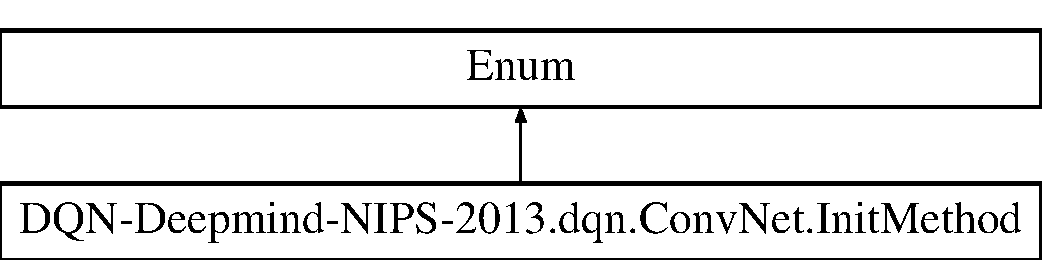
\includegraphics[height=2.000000cm]{classDQN-Deepmind-NIPS-2013_1_1dqn_1_1ConvNet_1_1InitMethod}
\end{center}
\end{figure}
\subsection*{Public Member Functions}
\begin{DoxyCompactItemize}
\item 
def \hyperlink{classDQN-Deepmind-NIPS-2013_1_1dqn_1_1ConvNet_1_1InitMethod_ae6c011ae724bdf51a3dc37c739170612}{is\+Valid} (e)
\begin{DoxyCompactList}\small\item\em The is\+Valid method check is the given value is a valid enumerated value. \end{DoxyCompactList}\end{DoxyCompactItemize}
\subsection*{Static Public Attributes}
\begin{DoxyCompactItemize}
\item 
int \hyperlink{classDQN-Deepmind-NIPS-2013_1_1dqn_1_1ConvNet_1_1InitMethod_ace1d7606694c2c82f5b4640a34b58a1c}{constant} = 0
\begin{DoxyCompactList}\small\item\em Initialize the variables with the given value. \end{DoxyCompactList}\item 
int \hyperlink{classDQN-Deepmind-NIPS-2013_1_1dqn_1_1ConvNet_1_1InitMethod_a40f9ca5144076077f6c2a28ca6983c1d}{xavier} = 1
\begin{DoxyCompactList}\small\item\em Perform a xavier initialization on the variables. \end{DoxyCompactList}\item 
int \hyperlink{classDQN-Deepmind-NIPS-2013_1_1dqn_1_1ConvNet_1_1InitMethod_ac26aff95fc96a42c00df1ef7cd7c7282}{uniform} = 2
\begin{DoxyCompactList}\small\item\em initialize the variables following a uniform distribution \end{DoxyCompactList}\item 
int \hyperlink{classDQN-Deepmind-NIPS-2013_1_1dqn_1_1ConvNet_1_1InitMethod_ad08fb9ba0ef227e2465bc0949566edac}{normal} = 3
\begin{DoxyCompactList}\small\item\em initialize the variables following a normal distribution \end{DoxyCompactList}\end{DoxyCompactItemize}


\subsection{Detailed Description}
The \hyperlink{classDQN-Deepmind-NIPS-2013_1_1dqn_1_1ConvNet_1_1InitMethod}{Init\+Method} inner is an enumeration of valid initialization for the functions \textquotesingle{}weights\textquotesingle{} and \textquotesingle{}biases\textquotesingle{}. 

\subsection{Member Function Documentation}
\hypertarget{classDQN-Deepmind-NIPS-2013_1_1dqn_1_1ConvNet_1_1InitMethod_ae6c011ae724bdf51a3dc37c739170612}{}\label{classDQN-Deepmind-NIPS-2013_1_1dqn_1_1ConvNet_1_1InitMethod_ae6c011ae724bdf51a3dc37c739170612} 
\index{D\+Q\+N-\/\+Deepmind-\/\+N\+I\+P\+S-\/2013\+::dqn\+::\+Conv\+Net\+::\+Init\+Method@{D\+Q\+N-\/\+Deepmind-\/\+N\+I\+P\+S-\/2013\+::dqn\+::\+Conv\+Net\+::\+Init\+Method}!is\+Valid@{is\+Valid}}
\index{is\+Valid@{is\+Valid}!D\+Q\+N-\/\+Deepmind-\/\+N\+I\+P\+S-\/2013\+::dqn\+::\+Conv\+Net\+::\+Init\+Method@{D\+Q\+N-\/\+Deepmind-\/\+N\+I\+P\+S-\/2013\+::dqn\+::\+Conv\+Net\+::\+Init\+Method}}
\subsubsection{\texorpdfstring{is\+Valid()}{isValid()}}
{\footnotesize\ttfamily def D\+QN-\/Deepmind-\/N\+I\+PS-\/2013.dqn.\+Conv\+Net.\+Init\+Method.\+is\+Valid (\begin{DoxyParamCaption}\item[{}]{e }\end{DoxyParamCaption})}



The is\+Valid method check is the given value is a valid enumerated value. 


\begin{DoxyParams}{Parameters}
{\em e} & \+: The value to check\\
\hline
\end{DoxyParams}
\begin{DoxyReturn}{Returns}
True if the given value is a valid initialization method or False otherwise 
\end{DoxyReturn}


\subsection{Member Data Documentation}
\hypertarget{classDQN-Deepmind-NIPS-2013_1_1dqn_1_1ConvNet_1_1InitMethod_ace1d7606694c2c82f5b4640a34b58a1c}{}\label{classDQN-Deepmind-NIPS-2013_1_1dqn_1_1ConvNet_1_1InitMethod_ace1d7606694c2c82f5b4640a34b58a1c} 
\index{D\+Q\+N-\/\+Deepmind-\/\+N\+I\+P\+S-\/2013\+::dqn\+::\+Conv\+Net\+::\+Init\+Method@{D\+Q\+N-\/\+Deepmind-\/\+N\+I\+P\+S-\/2013\+::dqn\+::\+Conv\+Net\+::\+Init\+Method}!constant@{constant}}
\index{constant@{constant}!D\+Q\+N-\/\+Deepmind-\/\+N\+I\+P\+S-\/2013\+::dqn\+::\+Conv\+Net\+::\+Init\+Method@{D\+Q\+N-\/\+Deepmind-\/\+N\+I\+P\+S-\/2013\+::dqn\+::\+Conv\+Net\+::\+Init\+Method}}
\subsubsection{\texorpdfstring{constant}{constant}}
{\footnotesize\ttfamily int D\+QN-\/Deepmind-\/N\+I\+PS-\/2013.dqn.\+Conv\+Net.\+Init\+Method.\+constant = 0\hspace{0.3cm}{\ttfamily [static]}}



Initialize the variables with the given value. 

\hypertarget{classDQN-Deepmind-NIPS-2013_1_1dqn_1_1ConvNet_1_1InitMethod_ad08fb9ba0ef227e2465bc0949566edac}{}\label{classDQN-Deepmind-NIPS-2013_1_1dqn_1_1ConvNet_1_1InitMethod_ad08fb9ba0ef227e2465bc0949566edac} 
\index{D\+Q\+N-\/\+Deepmind-\/\+N\+I\+P\+S-\/2013\+::dqn\+::\+Conv\+Net\+::\+Init\+Method@{D\+Q\+N-\/\+Deepmind-\/\+N\+I\+P\+S-\/2013\+::dqn\+::\+Conv\+Net\+::\+Init\+Method}!normal@{normal}}
\index{normal@{normal}!D\+Q\+N-\/\+Deepmind-\/\+N\+I\+P\+S-\/2013\+::dqn\+::\+Conv\+Net\+::\+Init\+Method@{D\+Q\+N-\/\+Deepmind-\/\+N\+I\+P\+S-\/2013\+::dqn\+::\+Conv\+Net\+::\+Init\+Method}}
\subsubsection{\texorpdfstring{normal}{normal}}
{\footnotesize\ttfamily int D\+QN-\/Deepmind-\/N\+I\+PS-\/2013.dqn.\+Conv\+Net.\+Init\+Method.\+normal = 3\hspace{0.3cm}{\ttfamily [static]}}



initialize the variables following a normal distribution 

\hypertarget{classDQN-Deepmind-NIPS-2013_1_1dqn_1_1ConvNet_1_1InitMethod_ac26aff95fc96a42c00df1ef7cd7c7282}{}\label{classDQN-Deepmind-NIPS-2013_1_1dqn_1_1ConvNet_1_1InitMethod_ac26aff95fc96a42c00df1ef7cd7c7282} 
\index{D\+Q\+N-\/\+Deepmind-\/\+N\+I\+P\+S-\/2013\+::dqn\+::\+Conv\+Net\+::\+Init\+Method@{D\+Q\+N-\/\+Deepmind-\/\+N\+I\+P\+S-\/2013\+::dqn\+::\+Conv\+Net\+::\+Init\+Method}!uniform@{uniform}}
\index{uniform@{uniform}!D\+Q\+N-\/\+Deepmind-\/\+N\+I\+P\+S-\/2013\+::dqn\+::\+Conv\+Net\+::\+Init\+Method@{D\+Q\+N-\/\+Deepmind-\/\+N\+I\+P\+S-\/2013\+::dqn\+::\+Conv\+Net\+::\+Init\+Method}}
\subsubsection{\texorpdfstring{uniform}{uniform}}
{\footnotesize\ttfamily int D\+QN-\/Deepmind-\/N\+I\+PS-\/2013.dqn.\+Conv\+Net.\+Init\+Method.\+uniform = 2\hspace{0.3cm}{\ttfamily [static]}}



initialize the variables following a uniform distribution 

\hypertarget{classDQN-Deepmind-NIPS-2013_1_1dqn_1_1ConvNet_1_1InitMethod_a40f9ca5144076077f6c2a28ca6983c1d}{}\label{classDQN-Deepmind-NIPS-2013_1_1dqn_1_1ConvNet_1_1InitMethod_a40f9ca5144076077f6c2a28ca6983c1d} 
\index{D\+Q\+N-\/\+Deepmind-\/\+N\+I\+P\+S-\/2013\+::dqn\+::\+Conv\+Net\+::\+Init\+Method@{D\+Q\+N-\/\+Deepmind-\/\+N\+I\+P\+S-\/2013\+::dqn\+::\+Conv\+Net\+::\+Init\+Method}!xavier@{xavier}}
\index{xavier@{xavier}!D\+Q\+N-\/\+Deepmind-\/\+N\+I\+P\+S-\/2013\+::dqn\+::\+Conv\+Net\+::\+Init\+Method@{D\+Q\+N-\/\+Deepmind-\/\+N\+I\+P\+S-\/2013\+::dqn\+::\+Conv\+Net\+::\+Init\+Method}}
\subsubsection{\texorpdfstring{xavier}{xavier}}
{\footnotesize\ttfamily int D\+QN-\/Deepmind-\/N\+I\+PS-\/2013.dqn.\+Conv\+Net.\+Init\+Method.\+xavier = 1\hspace{0.3cm}{\ttfamily [static]}}



Perform a xavier initialization on the variables. 



The documentation for this class was generated from the following file\+:\begin{DoxyCompactItemize}
\item 
dqn/\hyperlink{ConvNet_8py}{Conv\+Net.\+py}\end{DoxyCompactItemize}

\hypertarget{classDQN-Deepmind-NIPS-2013_1_1Message_1_1Message}{}\section{D\+Q\+N-\/\+Deepmind-\/\+N\+I\+P\+S-\/2013.Message.\+Message Class Reference}
\label{classDQN-Deepmind-NIPS-2013_1_1Message_1_1Message}\index{D\+Q\+N-\/\+Deepmind-\/\+N\+I\+P\+S-\/2013.\+Message.\+Message@{D\+Q\+N-\/\+Deepmind-\/\+N\+I\+P\+S-\/2013.\+Message.\+Message}}


The \hyperlink{classDQN-Deepmind-NIPS-2013_1_1Message_1_1Message}{Message} class overrides the threading.\+Event class to provide a simple way of communication between threads.  


Inheritance diagram for D\+Q\+N-\/\+Deepmind-\/\+N\+I\+P\+S-\/2013.Message.\+Message\+:\begin{figure}[H]
\begin{center}
\leavevmode
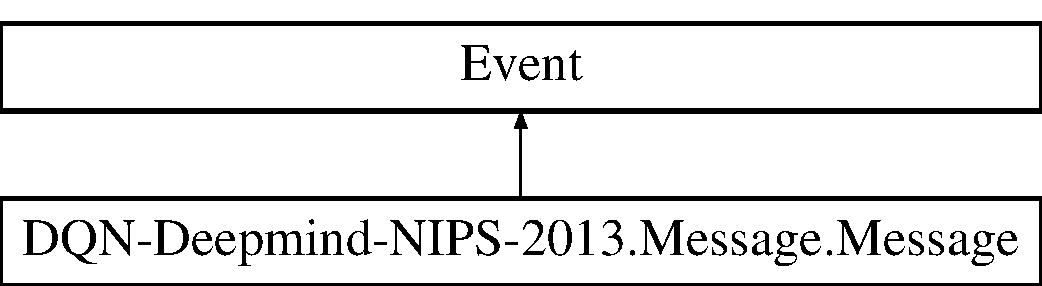
\includegraphics[height=2.000000cm]{classDQN-Deepmind-NIPS-2013_1_1Message_1_1Message}
\end{center}
\end{figure}
\subsection*{Public Member Functions}
\begin{DoxyCompactItemize}
\item 
def \hyperlink{classDQN-Deepmind-NIPS-2013_1_1Message_1_1Message_a2fdcb857df94a7edc9b6e36ef0a8e1c6}{\+\_\+\+\_\+init\+\_\+\+\_\+} (self)
\begin{DoxyCompactList}\small\item\em The \hyperlink{classDQN-Deepmind-NIPS-2013_1_1Message_1_1Message}{Message} class constructor. \end{DoxyCompactList}\item 
def \hyperlink{classDQN-Deepmind-NIPS-2013_1_1Message_1_1Message_a7f12ede11926bee5d5b3946375f28156}{read} (self)
\begin{DoxyCompactList}\small\item\em The read method reads the current message and reset the threading.\+Event internal flag. \end{DoxyCompactList}\item 
def \hyperlink{classDQN-Deepmind-NIPS-2013_1_1Message_1_1Message_a53cf5ac601122f2ace3178abee8f81db}{write} (self, message, data)
\begin{DoxyCompactList}\small\item\em The write method writes a message and set the threading.\+Event internal flag. \end{DoxyCompactList}\end{DoxyCompactItemize}
\subsection*{Static Public Attributes}
\begin{DoxyCompactItemize}
\item 
int \hyperlink{classDQN-Deepmind-NIPS-2013_1_1Message_1_1Message_a87173863ddcb622f03cefa6dcf9cda53}{Q\+U\+IT} = 0
\begin{DoxyCompactList}\small\item\em Default message type sent to aks the listenner to terminate. \end{DoxyCompactList}\item 
int \hyperlink{classDQN-Deepmind-NIPS-2013_1_1Message_1_1Message_a440cc65343a167377dae7c508e571c79}{T\+R\+A\+IN} = 1
\begin{DoxyCompactList}\small\item\em Default message type sent to ask the listenner to start trainind. \end{DoxyCompactList}\end{DoxyCompactItemize}


\subsection{Detailed Description}
The \hyperlink{classDQN-Deepmind-NIPS-2013_1_1Message_1_1Message}{Message} class overrides the threading.\+Event class to provide a simple way of communication between threads. 

\subsection{Constructor \& Destructor Documentation}
\hypertarget{classDQN-Deepmind-NIPS-2013_1_1Message_1_1Message_a2fdcb857df94a7edc9b6e36ef0a8e1c6}{}\label{classDQN-Deepmind-NIPS-2013_1_1Message_1_1Message_a2fdcb857df94a7edc9b6e36ef0a8e1c6} 
\index{D\+Q\+N-\/\+Deepmind-\/\+N\+I\+P\+S-\/2013\+::\+Message\+::\+Message@{D\+Q\+N-\/\+Deepmind-\/\+N\+I\+P\+S-\/2013\+::\+Message\+::\+Message}!\+\_\+\+\_\+init\+\_\+\+\_\+@{\+\_\+\+\_\+init\+\_\+\+\_\+}}
\index{\+\_\+\+\_\+init\+\_\+\+\_\+@{\+\_\+\+\_\+init\+\_\+\+\_\+}!D\+Q\+N-\/\+Deepmind-\/\+N\+I\+P\+S-\/2013\+::\+Message\+::\+Message@{D\+Q\+N-\/\+Deepmind-\/\+N\+I\+P\+S-\/2013\+::\+Message\+::\+Message}}
\subsubsection{\texorpdfstring{\+\_\+\+\_\+init\+\_\+\+\_\+()}{\_\_init\_\_()}}
{\footnotesize\ttfamily def D\+QN-\/Deepmind-\/N\+I\+PS-\/2013.Message.\+Message.\+\_\+\+\_\+init\+\_\+\+\_\+ (\begin{DoxyParamCaption}\item[{}]{self }\end{DoxyParamCaption})}



The \hyperlink{classDQN-Deepmind-NIPS-2013_1_1Message_1_1Message}{Message} class constructor. 



\subsection{Member Function Documentation}
\hypertarget{classDQN-Deepmind-NIPS-2013_1_1Message_1_1Message_a7f12ede11926bee5d5b3946375f28156}{}\label{classDQN-Deepmind-NIPS-2013_1_1Message_1_1Message_a7f12ede11926bee5d5b3946375f28156} 
\index{D\+Q\+N-\/\+Deepmind-\/\+N\+I\+P\+S-\/2013\+::\+Message\+::\+Message@{D\+Q\+N-\/\+Deepmind-\/\+N\+I\+P\+S-\/2013\+::\+Message\+::\+Message}!read@{read}}
\index{read@{read}!D\+Q\+N-\/\+Deepmind-\/\+N\+I\+P\+S-\/2013\+::\+Message\+::\+Message@{D\+Q\+N-\/\+Deepmind-\/\+N\+I\+P\+S-\/2013\+::\+Message\+::\+Message}}
\subsubsection{\texorpdfstring{read()}{read()}}
{\footnotesize\ttfamily def D\+QN-\/Deepmind-\/N\+I\+PS-\/2013.Message.\+Message.\+read (\begin{DoxyParamCaption}\item[{}]{self }\end{DoxyParamCaption})}



The read method reads the current message and reset the threading.\+Event internal flag. 

\begin{DoxyReturn}{Returns}
The registered message 
\end{DoxyReturn}
\hypertarget{classDQN-Deepmind-NIPS-2013_1_1Message_1_1Message_a53cf5ac601122f2ace3178abee8f81db}{}\label{classDQN-Deepmind-NIPS-2013_1_1Message_1_1Message_a53cf5ac601122f2ace3178abee8f81db} 
\index{D\+Q\+N-\/\+Deepmind-\/\+N\+I\+P\+S-\/2013\+::\+Message\+::\+Message@{D\+Q\+N-\/\+Deepmind-\/\+N\+I\+P\+S-\/2013\+::\+Message\+::\+Message}!write@{write}}
\index{write@{write}!D\+Q\+N-\/\+Deepmind-\/\+N\+I\+P\+S-\/2013\+::\+Message\+::\+Message@{D\+Q\+N-\/\+Deepmind-\/\+N\+I\+P\+S-\/2013\+::\+Message\+::\+Message}}
\subsubsection{\texorpdfstring{write()}{write()}}
{\footnotesize\ttfamily def D\+QN-\/Deepmind-\/N\+I\+PS-\/2013.Message.\+Message.\+write (\begin{DoxyParamCaption}\item[{}]{self,  }\item[{}]{message,  }\item[{}]{data }\end{DoxyParamCaption})}



The write method writes a message and set the threading.\+Event internal flag. 


\begin{DoxyParams}{Parameters}
{\em message} & \+: The message to send. \\
\hline
{\em data} & \+: Any additional datas associated to the message. This is not used for now \\
\hline
\end{DoxyParams}


\subsection{Member Data Documentation}
\hypertarget{classDQN-Deepmind-NIPS-2013_1_1Message_1_1Message_a87173863ddcb622f03cefa6dcf9cda53}{}\label{classDQN-Deepmind-NIPS-2013_1_1Message_1_1Message_a87173863ddcb622f03cefa6dcf9cda53} 
\index{D\+Q\+N-\/\+Deepmind-\/\+N\+I\+P\+S-\/2013\+::\+Message\+::\+Message@{D\+Q\+N-\/\+Deepmind-\/\+N\+I\+P\+S-\/2013\+::\+Message\+::\+Message}!Q\+U\+IT@{Q\+U\+IT}}
\index{Q\+U\+IT@{Q\+U\+IT}!D\+Q\+N-\/\+Deepmind-\/\+N\+I\+P\+S-\/2013\+::\+Message\+::\+Message@{D\+Q\+N-\/\+Deepmind-\/\+N\+I\+P\+S-\/2013\+::\+Message\+::\+Message}}
\subsubsection{\texorpdfstring{Q\+U\+IT}{QUIT}}
{\footnotesize\ttfamily int D\+QN-\/Deepmind-\/N\+I\+PS-\/2013.Message.\+Message.\+Q\+U\+IT = 0\hspace{0.3cm}{\ttfamily [static]}}



Default message type sent to aks the listenner to terminate. 

\hypertarget{classDQN-Deepmind-NIPS-2013_1_1Message_1_1Message_a440cc65343a167377dae7c508e571c79}{}\label{classDQN-Deepmind-NIPS-2013_1_1Message_1_1Message_a440cc65343a167377dae7c508e571c79} 
\index{D\+Q\+N-\/\+Deepmind-\/\+N\+I\+P\+S-\/2013\+::\+Message\+::\+Message@{D\+Q\+N-\/\+Deepmind-\/\+N\+I\+P\+S-\/2013\+::\+Message\+::\+Message}!T\+R\+A\+IN@{T\+R\+A\+IN}}
\index{T\+R\+A\+IN@{T\+R\+A\+IN}!D\+Q\+N-\/\+Deepmind-\/\+N\+I\+P\+S-\/2013\+::\+Message\+::\+Message@{D\+Q\+N-\/\+Deepmind-\/\+N\+I\+P\+S-\/2013\+::\+Message\+::\+Message}}
\subsubsection{\texorpdfstring{T\+R\+A\+IN}{TRAIN}}
{\footnotesize\ttfamily int D\+QN-\/Deepmind-\/N\+I\+PS-\/2013.Message.\+Message.\+T\+R\+A\+IN = 1\hspace{0.3cm}{\ttfamily [static]}}



Default message type sent to ask the listenner to start trainind. 



The documentation for this class was generated from the following file\+:\begin{DoxyCompactItemize}
\item 
\hyperlink{Message_8py}{Message.\+py}\end{DoxyCompactItemize}

\hypertarget{classDQN-Deepmind-NIPS-2013_1_1dqn_1_1ConvNet_1_1Paddings}{}\section{D\+Q\+N-\/\+Deepmind-\/\+N\+I\+P\+S-\/2013.dqn.\+Conv\+Net.\+Paddings Class Reference}
\label{classDQN-Deepmind-NIPS-2013_1_1dqn_1_1ConvNet_1_1Paddings}\index{D\+Q\+N-\/\+Deepmind-\/\+N\+I\+P\+S-\/2013.\+dqn.\+Conv\+Net.\+Paddings@{D\+Q\+N-\/\+Deepmind-\/\+N\+I\+P\+S-\/2013.\+dqn.\+Conv\+Net.\+Paddings}}


The \hyperlink{classDQN-Deepmind-NIPS-2013_1_1dqn_1_1ConvNet_1_1Paddings}{Paddings} class enumerates the valid values for padding.  


Inheritance diagram for D\+Q\+N-\/\+Deepmind-\/\+N\+I\+P\+S-\/2013.dqn.\+Conv\+Net.\+Paddings\+:\begin{figure}[H]
\begin{center}
\leavevmode
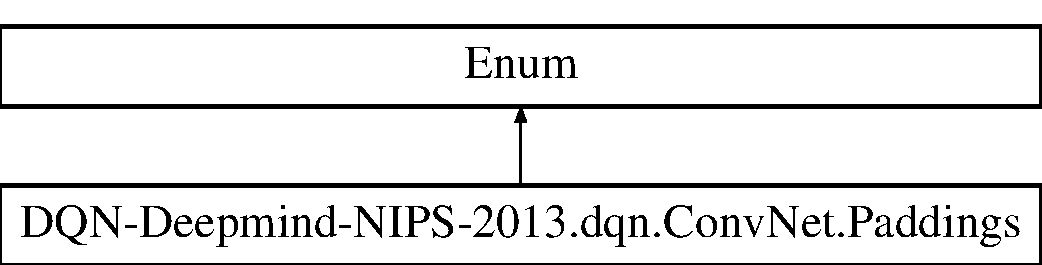
\includegraphics[height=2.000000cm]{classDQN-Deepmind-NIPS-2013_1_1dqn_1_1ConvNet_1_1Paddings}
\end{center}
\end{figure}
\subsection*{Public Member Functions}
\begin{DoxyCompactItemize}
\item 
def \hyperlink{classDQN-Deepmind-NIPS-2013_1_1dqn_1_1ConvNet_1_1Paddings_a0d529b649569466ae860a5d9f0556f79}{is\+Valid} (e)
\begin{DoxyCompactList}\small\item\em The is\+Valid method check is the given value is a valid enumerated value. \end{DoxyCompactList}\item 
def \hyperlink{classDQN-Deepmind-NIPS-2013_1_1dqn_1_1ConvNet_1_1Paddings_a06c639bace15b03e0e397b090c989ba6}{output\+Shape} (input\+Shape, filters, fH, fW, vS, hS, p)
\begin{DoxyCompactList}\small\item\em The output\+Shape compute the shape of the output of a convolutional layer set up with the given attributes. \end{DoxyCompactList}\end{DoxyCompactItemize}
\subsection*{Static Public Attributes}
\begin{DoxyCompactItemize}
\item 
string \hyperlink{classDQN-Deepmind-NIPS-2013_1_1dqn_1_1ConvNet_1_1Paddings_a7c3a65b0f0b21e5106a02ad146534d4d}{valid} = \char`\"{}valid\char`\"{}
\item 
string \hyperlink{classDQN-Deepmind-NIPS-2013_1_1dqn_1_1ConvNet_1_1Paddings_a4a1207898291d64aa30616f671eadffd}{full} = \char`\"{}full\char`\"{}
\item 
string \hyperlink{classDQN-Deepmind-NIPS-2013_1_1dqn_1_1ConvNet_1_1Paddings_aee5f886e1f925c58efddcfbb734c57fc}{half} = \char`\"{}half\char`\"{}
\end{DoxyCompactItemize}


\subsection{Detailed Description}
The \hyperlink{classDQN-Deepmind-NIPS-2013_1_1dqn_1_1ConvNet_1_1Paddings}{Paddings} class enumerates the valid values for padding. 

\begin{DoxySeeAlso}{See also}
\href{http://deeplearning.net/software/theano_versions/dev/library/tensor/nnet/conv.html#theano.tensor.nnet.conv2d}{\tt theano.\+tensor.\+nnet.\+conv2d} 
\end{DoxySeeAlso}


\subsection{Member Function Documentation}
\hypertarget{classDQN-Deepmind-NIPS-2013_1_1dqn_1_1ConvNet_1_1Paddings_a0d529b649569466ae860a5d9f0556f79}{}\label{classDQN-Deepmind-NIPS-2013_1_1dqn_1_1ConvNet_1_1Paddings_a0d529b649569466ae860a5d9f0556f79} 
\index{D\+Q\+N-\/\+Deepmind-\/\+N\+I\+P\+S-\/2013\+::dqn\+::\+Conv\+Net\+::\+Paddings@{D\+Q\+N-\/\+Deepmind-\/\+N\+I\+P\+S-\/2013\+::dqn\+::\+Conv\+Net\+::\+Paddings}!is\+Valid@{is\+Valid}}
\index{is\+Valid@{is\+Valid}!D\+Q\+N-\/\+Deepmind-\/\+N\+I\+P\+S-\/2013\+::dqn\+::\+Conv\+Net\+::\+Paddings@{D\+Q\+N-\/\+Deepmind-\/\+N\+I\+P\+S-\/2013\+::dqn\+::\+Conv\+Net\+::\+Paddings}}
\subsubsection{\texorpdfstring{is\+Valid()}{isValid()}}
{\footnotesize\ttfamily def D\+QN-\/Deepmind-\/N\+I\+PS-\/2013.dqn.\+Conv\+Net.\+Paddings.\+is\+Valid (\begin{DoxyParamCaption}\item[{}]{e }\end{DoxyParamCaption})}



The is\+Valid method check is the given value is a valid enumerated value. 


\begin{DoxyParams}{Parameters}
{\em e} & \+: The value to check\\
\hline
\end{DoxyParams}
\begin{DoxyReturn}{Returns}
True if the given value is a valid padding value or False otherwise 
\end{DoxyReturn}
\hypertarget{classDQN-Deepmind-NIPS-2013_1_1dqn_1_1ConvNet_1_1Paddings_a06c639bace15b03e0e397b090c989ba6}{}\label{classDQN-Deepmind-NIPS-2013_1_1dqn_1_1ConvNet_1_1Paddings_a06c639bace15b03e0e397b090c989ba6} 
\index{D\+Q\+N-\/\+Deepmind-\/\+N\+I\+P\+S-\/2013\+::dqn\+::\+Conv\+Net\+::\+Paddings@{D\+Q\+N-\/\+Deepmind-\/\+N\+I\+P\+S-\/2013\+::dqn\+::\+Conv\+Net\+::\+Paddings}!output\+Shape@{output\+Shape}}
\index{output\+Shape@{output\+Shape}!D\+Q\+N-\/\+Deepmind-\/\+N\+I\+P\+S-\/2013\+::dqn\+::\+Conv\+Net\+::\+Paddings@{D\+Q\+N-\/\+Deepmind-\/\+N\+I\+P\+S-\/2013\+::dqn\+::\+Conv\+Net\+::\+Paddings}}
\subsubsection{\texorpdfstring{output\+Shape()}{outputShape()}}
{\footnotesize\ttfamily def D\+QN-\/Deepmind-\/N\+I\+PS-\/2013.dqn.\+Conv\+Net.\+Paddings.\+output\+Shape (\begin{DoxyParamCaption}\item[{}]{input\+Shape,  }\item[{}]{filters,  }\item[{}]{fH,  }\item[{}]{fW,  }\item[{}]{vS,  }\item[{}]{hS,  }\item[{}]{p }\end{DoxyParamCaption})}



The output\+Shape compute the shape of the output of a convolutional layer set up with the given attributes. 


\begin{DoxyParams}{Parameters}
{\em input\+Shape} & \+: The shape of the input passed to the layer \\
\hline
{\em filters} & \+: The number of filters \\
\hline
{\em fH} & \+: The height of the filters \\
\hline
{\em fW} & \+: The width of the filters \\
\hline
{\em vS} & \+: The vertical stride \\
\hline
{\em hS} & \+: The horizontal stride \\
\hline
{\em p} & \+: The padding applied to the input before performing the convolution\\
\hline
\end{DoxyParams}
\begin{DoxyReturn}{Returns}
A four entries list representing the computed shape 
\end{DoxyReturn}


\subsection{Member Data Documentation}
\hypertarget{classDQN-Deepmind-NIPS-2013_1_1dqn_1_1ConvNet_1_1Paddings_a4a1207898291d64aa30616f671eadffd}{}\label{classDQN-Deepmind-NIPS-2013_1_1dqn_1_1ConvNet_1_1Paddings_a4a1207898291d64aa30616f671eadffd} 
\index{D\+Q\+N-\/\+Deepmind-\/\+N\+I\+P\+S-\/2013\+::dqn\+::\+Conv\+Net\+::\+Paddings@{D\+Q\+N-\/\+Deepmind-\/\+N\+I\+P\+S-\/2013\+::dqn\+::\+Conv\+Net\+::\+Paddings}!full@{full}}
\index{full@{full}!D\+Q\+N-\/\+Deepmind-\/\+N\+I\+P\+S-\/2013\+::dqn\+::\+Conv\+Net\+::\+Paddings@{D\+Q\+N-\/\+Deepmind-\/\+N\+I\+P\+S-\/2013\+::dqn\+::\+Conv\+Net\+::\+Paddings}}
\subsubsection{\texorpdfstring{full}{full}}
{\footnotesize\ttfamily string D\+QN-\/Deepmind-\/N\+I\+PS-\/2013.dqn.\+Conv\+Net.\+Paddings.\+full = \char`\"{}full\char`\"{}\hspace{0.3cm}{\ttfamily [static]}}

\hypertarget{classDQN-Deepmind-NIPS-2013_1_1dqn_1_1ConvNet_1_1Paddings_aee5f886e1f925c58efddcfbb734c57fc}{}\label{classDQN-Deepmind-NIPS-2013_1_1dqn_1_1ConvNet_1_1Paddings_aee5f886e1f925c58efddcfbb734c57fc} 
\index{D\+Q\+N-\/\+Deepmind-\/\+N\+I\+P\+S-\/2013\+::dqn\+::\+Conv\+Net\+::\+Paddings@{D\+Q\+N-\/\+Deepmind-\/\+N\+I\+P\+S-\/2013\+::dqn\+::\+Conv\+Net\+::\+Paddings}!half@{half}}
\index{half@{half}!D\+Q\+N-\/\+Deepmind-\/\+N\+I\+P\+S-\/2013\+::dqn\+::\+Conv\+Net\+::\+Paddings@{D\+Q\+N-\/\+Deepmind-\/\+N\+I\+P\+S-\/2013\+::dqn\+::\+Conv\+Net\+::\+Paddings}}
\subsubsection{\texorpdfstring{half}{half}}
{\footnotesize\ttfamily string D\+QN-\/Deepmind-\/N\+I\+PS-\/2013.dqn.\+Conv\+Net.\+Paddings.\+half = \char`\"{}half\char`\"{}\hspace{0.3cm}{\ttfamily [static]}}

\hypertarget{classDQN-Deepmind-NIPS-2013_1_1dqn_1_1ConvNet_1_1Paddings_a7c3a65b0f0b21e5106a02ad146534d4d}{}\label{classDQN-Deepmind-NIPS-2013_1_1dqn_1_1ConvNet_1_1Paddings_a7c3a65b0f0b21e5106a02ad146534d4d} 
\index{D\+Q\+N-\/\+Deepmind-\/\+N\+I\+P\+S-\/2013\+::dqn\+::\+Conv\+Net\+::\+Paddings@{D\+Q\+N-\/\+Deepmind-\/\+N\+I\+P\+S-\/2013\+::dqn\+::\+Conv\+Net\+::\+Paddings}!valid@{valid}}
\index{valid@{valid}!D\+Q\+N-\/\+Deepmind-\/\+N\+I\+P\+S-\/2013\+::dqn\+::\+Conv\+Net\+::\+Paddings@{D\+Q\+N-\/\+Deepmind-\/\+N\+I\+P\+S-\/2013\+::dqn\+::\+Conv\+Net\+::\+Paddings}}
\subsubsection{\texorpdfstring{valid}{valid}}
{\footnotesize\ttfamily string D\+QN-\/Deepmind-\/N\+I\+PS-\/2013.dqn.\+Conv\+Net.\+Paddings.\+valid = \char`\"{}valid\char`\"{}\hspace{0.3cm}{\ttfamily [static]}}



The documentation for this class was generated from the following file\+:\begin{DoxyCompactItemize}
\item 
dqn/\hyperlink{ConvNet_8py}{Conv\+Net.\+py}\end{DoxyCompactItemize}

\hypertarget{classDQN-Deepmind-NIPS-2013_1_1Plotter_1_1Plotter}{}\section{D\+Q\+N-\/\+Deepmind-\/\+N\+I\+P\+S-\/2013.Plotter.\+Plotter Class Reference}
\label{classDQN-Deepmind-NIPS-2013_1_1Plotter_1_1Plotter}\index{D\+Q\+N-\/\+Deepmind-\/\+N\+I\+P\+S-\/2013.\+Plotter.\+Plotter@{D\+Q\+N-\/\+Deepmind-\/\+N\+I\+P\+S-\/2013.\+Plotter.\+Plotter}}


The \hyperlink{classDQN-Deepmind-NIPS-2013_1_1Plotter_1_1Plotter}{Plotter} Class provides an easy way to plot lines and distributions.  


Inheritance diagram for D\+Q\+N-\/\+Deepmind-\/\+N\+I\+P\+S-\/2013.Plotter.\+Plotter\+:\begin{figure}[H]
\begin{center}
\leavevmode
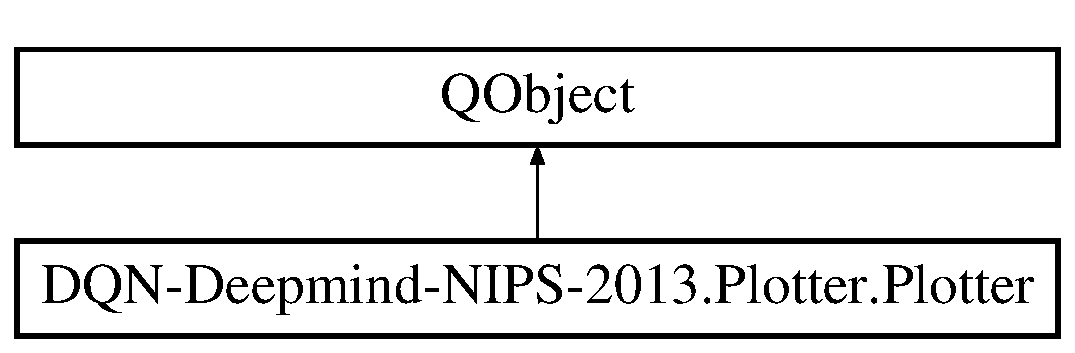
\includegraphics[height=2.000000cm]{classDQN-Deepmind-NIPS-2013_1_1Plotter_1_1Plotter}
\end{center}
\end{figure}
\subsection*{Public Member Functions}
\begin{DoxyCompactItemize}
\item 
def \hyperlink{classDQN-Deepmind-NIPS-2013_1_1Plotter_1_1Plotter_a781363a311a4b659f454b9f10a930fe5}{rand\+Color} ()
\begin{DoxyCompactList}\small\item\em The rand\+Color static method computes and returns a random color. \end{DoxyCompactList}\item 
def \hyperlink{classDQN-Deepmind-NIPS-2013_1_1Plotter_1_1Plotter_a667c98c2620e83ae62d8cd9a9ba4e94c}{\+\_\+\+\_\+init\+\_\+\+\_\+} (self)
\begin{DoxyCompactList}\small\item\em The \hyperlink{classDQN-Deepmind-NIPS-2013_1_1Plotter_1_1Plotter}{Plotter} constructor. \end{DoxyCompactList}\item 
def \hyperlink{classDQN-Deepmind-NIPS-2013_1_1Plotter_1_1Plotter_a8e1227cf851a49de8362084fe06846fa}{initialize} (self)
\begin{DoxyCompactList}\small\item\em The initialize method initializes the \hyperlink{classDQN-Deepmind-NIPS-2013_1_1Plotter_1_1Plotter}{Plotter} class. \end{DoxyCompactList}\item 
def \hyperlink{classDQN-Deepmind-NIPS-2013_1_1Plotter_1_1Plotter_a5369f165b720b7867e35cb1394d1a4f7}{connect\+Signals} (self)
\begin{DoxyCompactList}\small\item\em The connect\+Signals connects the signals to the rights methods. \end{DoxyCompactList}\item 
def \hyperlink{classDQN-Deepmind-NIPS-2013_1_1Plotter_1_1Plotter_a289c6002e292a7c4b60e335bddbd9ae0}{add\+Group} (self, name)
\begin{DoxyCompactList}\small\item\em The add\+Group method add the given group to the list. \end{DoxyCompactList}\item 
def \hyperlink{classDQN-Deepmind-NIPS-2013_1_1Plotter_1_1Plotter_ac7b49118b884b5203067c4f976cc6158}{del\+Group} (self, name)
\begin{DoxyCompactList}\small\item\em The del\+Group method delete the given group. \end{DoxyCompactList}\item 
def \hyperlink{classDQN-Deepmind-NIPS-2013_1_1Plotter_1_1Plotter_aafcbaaa8995b5e9f2859f25187895248}{add\+Plot} (self, group, name, cnt, styles)
\begin{DoxyCompactList}\small\item\em The add\+Plot method adds a plot to the given group. \end{DoxyCompactList}\item 
def \hyperlink{classDQN-Deepmind-NIPS-2013_1_1Plotter_1_1Plotter_ae8f20f0c734fc1447e4093638ac8b40f}{add\+Percentile} (self, group, name, percentages\+Pairs)
\begin{DoxyCompactList}\small\item\em The add\+Percentile methods add a percentile chart to the list. \end{DoxyCompactList}\item 
def \hyperlink{classDQN-Deepmind-NIPS-2013_1_1Plotter_1_1Plotter_acc6be1793e58dc9a665702177dae7cdb}{update\+Plot} (self, group, name, x, y\+Values)
\begin{DoxyCompactList}\small\item\em The update\+Plot method updates the given plot with the given coordinates. \end{DoxyCompactList}\item 
def \hyperlink{classDQN-Deepmind-NIPS-2013_1_1Plotter_1_1Plotter_a9efb9a96e31b427d493d434970279c51}{update\+Percentile} (self, group, name, x, values)
\begin{DoxyCompactList}\small\item\em The update\+Percentile method updates the given percentile plot. \end{DoxyCompactList}\end{DoxyCompactItemize}
\subsection*{Static Public Attributes}
\begin{DoxyCompactItemize}
\item 
int \hyperlink{classDQN-Deepmind-NIPS-2013_1_1Plotter_1_1Plotter_a0ed150721300639b6230824109f7427b}{P\+L\+OT} = 0
\begin{DoxyCompactList}\small\item\em Usual plot type. \end{DoxyCompactList}\item 
int \hyperlink{classDQN-Deepmind-NIPS-2013_1_1Plotter_1_1Plotter_a1f89ddbef8de94b70bfce1c5c6427b4b}{P\+E\+RC} = 1
\begin{DoxyCompactList}\small\item\em Percentile plot type. \end{DoxyCompactList}\item 
\hyperlink{classDQN-Deepmind-NIPS-2013_1_1Plotter_1_1Plotter_ac731a7755fab8cf0958411b81af56f55}{G\+R\+P\+\_\+\+F\+O\+N\+TS} = qtg.\+Q\+Font(\char`\"{}\char`\"{}, -\/1, qtg.\+Q\+Font.\+Black, False)
\begin{DoxyCompactList}\small\item\em Font used to display the groups in the list. \end{DoxyCompactList}\item 
\hyperlink{classDQN-Deepmind-NIPS-2013_1_1Plotter_1_1Plotter_a526f4f1265860b0186b6232689de6335}{E\+R\+R\+O\+R\+\_\+\+F\+O\+N\+TS} = qtg.\+Q\+Font(\char`\"{}\char`\"{}, -\/1, qtg.\+Q\+Font.\+Bold , False)
\begin{DoxyCompactList}\small\item\em Font used to display an error. \end{DoxyCompactList}\item 
\hyperlink{classDQN-Deepmind-NIPS-2013_1_1Plotter_1_1Plotter_a6b90920063b98d9487ba14c48f5af362}{P\+L\+T\+\_\+\+F\+O\+N\+TS} = qtg.\+Q\+Font()
\begin{DoxyCompactList}\small\item\em Font used to display a plot in the list. \end{DoxyCompactList}\item 
\hyperlink{classDQN-Deepmind-NIPS-2013_1_1Plotter_1_1Plotter_a9e65187d496ef975f211f37ec66f77b0}{S\+U\+B\+\_\+\+P\+L\+T\+\_\+\+F\+O\+N\+TS} = qtg.\+Q\+Font()
\begin{DoxyCompactList}\small\item\em Font used to display a subplot in the subplot list. \end{DoxyCompactList}\item 
\hyperlink{classDQN-Deepmind-NIPS-2013_1_1Plotter_1_1Plotter_aa599f9c39b850680c4842b8a53268882}{P\+E\+R\+\_\+\+C\+O\+L\+OR} = pg.\+mk\+Color(\char`\"{}\#ff7500\char`\"{})
\begin{DoxyCompactList}\small\item\em Basic color used in the percentile charts. \end{DoxyCompactList}\item 
\hyperlink{classDQN-Deepmind-NIPS-2013_1_1Plotter_1_1Plotter_aa272066f3775c7e5a00e58664498b545}{F\+G\+\_\+\+E\+R\+R\+\_\+\+C\+O\+L\+OR} = pg.\+mk\+Color(\char`\"{}\#ff3e04\char`\"{})
\begin{DoxyCompactList}\small\item\em Color used to display an error. \end{DoxyCompactList}\item 
\hyperlink{classDQN-Deepmind-NIPS-2013_1_1Plotter_1_1Plotter_a49bdb6a37de2bcff4d702417c64105ff}{G\+R\+P\+\_\+\+R\+O\+LE} = qtc.\+Qt.\+User\+Role
\begin{DoxyCompactList}\small\item\em \textquotesingle{}Role\textquotesingle{} id for the group name \end{DoxyCompactList}\item 
int \hyperlink{classDQN-Deepmind-NIPS-2013_1_1Plotter_1_1Plotter_aaedbcbba023e3d7730beb86579ec7efe}{P\+L\+T\+\_\+\+R\+O\+LE} = qtc.\+Qt.\+User\+Role + 1
\begin{DoxyCompactList}\small\item\em \textquotesingle{}Role\textquotesingle{} id for the plot name \end{DoxyCompactList}\item 
int \hyperlink{classDQN-Deepmind-NIPS-2013_1_1Plotter_1_1Plotter_ae72b47c3cf2965e2aca86ee30256edea}{E\+R\+R\+O\+R\+\_\+\+R\+O\+LE} = qtc.\+Qt.\+User\+Role + 2
\begin{DoxyCompactList}\small\item\em \textquotesingle{}Role\textquotesingle{} id that indicates if an error already arised or not \end{DoxyCompactList}\item 
int \hyperlink{classDQN-Deepmind-NIPS-2013_1_1Plotter_1_1Plotter_a7f8f653368bc22c7e80147b1d8dc5f18}{S\+U\+B\+\_\+\+ID} = qtc.\+Qt.\+User\+Role + 3
\begin{DoxyCompactList}\small\item\em \textquotesingle{}Role\textquotesingle{} id for the subplot id \end{DoxyCompactList}\item 
\hyperlink{classDQN-Deepmind-NIPS-2013_1_1Plotter_1_1Plotter_aa6b7419c1641e98f1d050f4553becaf2}{update\+\_\+list\+\_\+sig} = qtc.\+pyqt\+Signal()
\begin{DoxyCompactList}\small\item\em Signal used to ask the plotting thread to update the list of plots. \end{DoxyCompactList}\item 
\hyperlink{classDQN-Deepmind-NIPS-2013_1_1Plotter_1_1Plotter_af89689f9142da4126b9c256efa69bec6}{update\+\_\+plot\+\_\+sig} = qtc.\+pyqt\+Signal(str, str)
\begin{DoxyCompactList}\small\item\em Signal used to ask the plotting thread to update a plot. \end{DoxyCompactList}\item 
\hyperlink{classDQN-Deepmind-NIPS-2013_1_1Plotter_1_1Plotter_a4d72a490c71c0bb118e8c76a665a4908}{update\+\_\+percentile\+\_\+sig} = qtc.\+pyqt\+Signal(str, str)
\begin{DoxyCompactList}\small\item\em Signal used to ask the plotting thread to update a percetile plot. \end{DoxyCompactList}\end{DoxyCompactItemize}


\subsection{Detailed Description}
The \hyperlink{classDQN-Deepmind-NIPS-2013_1_1Plotter_1_1Plotter}{Plotter} Class provides an easy way to plot lines and distributions. 

\subsection{Constructor \& Destructor Documentation}
\hypertarget{classDQN-Deepmind-NIPS-2013_1_1Plotter_1_1Plotter_a667c98c2620e83ae62d8cd9a9ba4e94c}{}\label{classDQN-Deepmind-NIPS-2013_1_1Plotter_1_1Plotter_a667c98c2620e83ae62d8cd9a9ba4e94c} 
\index{D\+Q\+N-\/\+Deepmind-\/\+N\+I\+P\+S-\/2013\+::\+Plotter\+::\+Plotter@{D\+Q\+N-\/\+Deepmind-\/\+N\+I\+P\+S-\/2013\+::\+Plotter\+::\+Plotter}!\+\_\+\+\_\+init\+\_\+\+\_\+@{\+\_\+\+\_\+init\+\_\+\+\_\+}}
\index{\+\_\+\+\_\+init\+\_\+\+\_\+@{\+\_\+\+\_\+init\+\_\+\+\_\+}!D\+Q\+N-\/\+Deepmind-\/\+N\+I\+P\+S-\/2013\+::\+Plotter\+::\+Plotter@{D\+Q\+N-\/\+Deepmind-\/\+N\+I\+P\+S-\/2013\+::\+Plotter\+::\+Plotter}}
\subsubsection{\texorpdfstring{\+\_\+\+\_\+init\+\_\+\+\_\+()}{\_\_init\_\_()}}
{\footnotesize\ttfamily def D\+QN-\/Deepmind-\/N\+I\+PS-\/2013.Plotter.\+Plotter.\+\_\+\+\_\+init\+\_\+\+\_\+ (\begin{DoxyParamCaption}\item[{}]{self }\end{DoxyParamCaption})}



The \hyperlink{classDQN-Deepmind-NIPS-2013_1_1Plotter_1_1Plotter}{Plotter} constructor. 



\subsection{Member Function Documentation}
\hypertarget{classDQN-Deepmind-NIPS-2013_1_1Plotter_1_1Plotter_a289c6002e292a7c4b60e335bddbd9ae0}{}\label{classDQN-Deepmind-NIPS-2013_1_1Plotter_1_1Plotter_a289c6002e292a7c4b60e335bddbd9ae0} 
\index{D\+Q\+N-\/\+Deepmind-\/\+N\+I\+P\+S-\/2013\+::\+Plotter\+::\+Plotter@{D\+Q\+N-\/\+Deepmind-\/\+N\+I\+P\+S-\/2013\+::\+Plotter\+::\+Plotter}!add\+Group@{add\+Group}}
\index{add\+Group@{add\+Group}!D\+Q\+N-\/\+Deepmind-\/\+N\+I\+P\+S-\/2013\+::\+Plotter\+::\+Plotter@{D\+Q\+N-\/\+Deepmind-\/\+N\+I\+P\+S-\/2013\+::\+Plotter\+::\+Plotter}}
\subsubsection{\texorpdfstring{add\+Group()}{addGroup()}}
{\footnotesize\ttfamily def D\+QN-\/Deepmind-\/N\+I\+PS-\/2013.Plotter.\+Plotter.\+add\+Group (\begin{DoxyParamCaption}\item[{}]{self,  }\item[{}]{name }\end{DoxyParamCaption})}



The add\+Group method add the given group to the list. 


\begin{DoxyParams}{Parameters}
{\em name} & \+: The name of the group to add \\
\hline
\end{DoxyParams}
\hypertarget{classDQN-Deepmind-NIPS-2013_1_1Plotter_1_1Plotter_ae8f20f0c734fc1447e4093638ac8b40f}{}\label{classDQN-Deepmind-NIPS-2013_1_1Plotter_1_1Plotter_ae8f20f0c734fc1447e4093638ac8b40f} 
\index{D\+Q\+N-\/\+Deepmind-\/\+N\+I\+P\+S-\/2013\+::\+Plotter\+::\+Plotter@{D\+Q\+N-\/\+Deepmind-\/\+N\+I\+P\+S-\/2013\+::\+Plotter\+::\+Plotter}!add\+Percentile@{add\+Percentile}}
\index{add\+Percentile@{add\+Percentile}!D\+Q\+N-\/\+Deepmind-\/\+N\+I\+P\+S-\/2013\+::\+Plotter\+::\+Plotter@{D\+Q\+N-\/\+Deepmind-\/\+N\+I\+P\+S-\/2013\+::\+Plotter\+::\+Plotter}}
\subsubsection{\texorpdfstring{add\+Percentile()}{addPercentile()}}
{\footnotesize\ttfamily def D\+QN-\/Deepmind-\/N\+I\+PS-\/2013.Plotter.\+Plotter.\+add\+Percentile (\begin{DoxyParamCaption}\item[{}]{self,  }\item[{}]{group,  }\item[{}]{name,  }\item[{}]{percentages\+Pairs }\end{DoxyParamCaption})}



The add\+Percentile methods add a percentile chart to the list. 


\begin{DoxyParams}{Parameters}
{\em group} & \+: The name of the group the percentile chart belongs to \\
\hline
{\em name} & \+: The name of the chart \\
\hline
{\em percentages\+Pairs} & \+: A list of tuple of values between and including 0 and 100. If percentages\+Pairs is made of pairs (p\+\_\+i, p\+\_\+j) the chart will be made of \+:
\begin{DoxyItemize}
\item A line at (x, percentile(\+A(x), p\+\_\+i))
\item A line at (x, percentile(\+A(x), p\+\_\+j))
\item An area filled between the two previous lines with color where the alpha value is proportional to p\+\_\+i -\/ p\+\_\+j 
\end{DoxyItemize}\\
\hline
\end{DoxyParams}
\hypertarget{classDQN-Deepmind-NIPS-2013_1_1Plotter_1_1Plotter_aafcbaaa8995b5e9f2859f25187895248}{}\label{classDQN-Deepmind-NIPS-2013_1_1Plotter_1_1Plotter_aafcbaaa8995b5e9f2859f25187895248} 
\index{D\+Q\+N-\/\+Deepmind-\/\+N\+I\+P\+S-\/2013\+::\+Plotter\+::\+Plotter@{D\+Q\+N-\/\+Deepmind-\/\+N\+I\+P\+S-\/2013\+::\+Plotter\+::\+Plotter}!add\+Plot@{add\+Plot}}
\index{add\+Plot@{add\+Plot}!D\+Q\+N-\/\+Deepmind-\/\+N\+I\+P\+S-\/2013\+::\+Plotter\+::\+Plotter@{D\+Q\+N-\/\+Deepmind-\/\+N\+I\+P\+S-\/2013\+::\+Plotter\+::\+Plotter}}
\subsubsection{\texorpdfstring{add\+Plot()}{addPlot()}}
{\footnotesize\ttfamily def D\+QN-\/Deepmind-\/N\+I\+PS-\/2013.Plotter.\+Plotter.\+add\+Plot (\begin{DoxyParamCaption}\item[{}]{self,  }\item[{}]{group,  }\item[{}]{name,  }\item[{}]{cnt,  }\item[{}]{styles }\end{DoxyParamCaption})}



The add\+Plot method adds a plot to the given group. 


\begin{DoxyParams}{Parameters}
{\em group} & \+: The name of the group the plot belongs to \\
\hline
{\em name} & \+: The name of the new plot to add. This name should be unique inside the given group \\
\hline
{\em cnt} & \+: How many lines will be plotted at the same time \\
\hline
{\em styles} & \+: The style of the lines to plot. Styles must have \textquotesingle{}cnt\textquotesingle{} elements. The elements in \textquotesingle{}styles\textquotesingle{} will be directly passed to \textquotesingle{}pyqtgraph.\+mk\+Pen\textquotesingle{}. See \href{http://www.pyqtgraph.org/documentation/functions.html?highlight=mkpen#pyqtgraph.mkPen}{\tt pyqtgraph.\+mk\+Pen} documentaiton for more information \\
\hline
\end{DoxyParams}
\hypertarget{classDQN-Deepmind-NIPS-2013_1_1Plotter_1_1Plotter_a5369f165b720b7867e35cb1394d1a4f7}{}\label{classDQN-Deepmind-NIPS-2013_1_1Plotter_1_1Plotter_a5369f165b720b7867e35cb1394d1a4f7} 
\index{D\+Q\+N-\/\+Deepmind-\/\+N\+I\+P\+S-\/2013\+::\+Plotter\+::\+Plotter@{D\+Q\+N-\/\+Deepmind-\/\+N\+I\+P\+S-\/2013\+::\+Plotter\+::\+Plotter}!connect\+Signals@{connect\+Signals}}
\index{connect\+Signals@{connect\+Signals}!D\+Q\+N-\/\+Deepmind-\/\+N\+I\+P\+S-\/2013\+::\+Plotter\+::\+Plotter@{D\+Q\+N-\/\+Deepmind-\/\+N\+I\+P\+S-\/2013\+::\+Plotter\+::\+Plotter}}
\subsubsection{\texorpdfstring{connect\+Signals()}{connectSignals()}}
{\footnotesize\ttfamily def D\+QN-\/Deepmind-\/N\+I\+PS-\/2013.Plotter.\+Plotter.\+connect\+Signals (\begin{DoxyParamCaption}\item[{}]{self }\end{DoxyParamCaption})}



The connect\+Signals connects the signals to the rights methods. 

\hypertarget{classDQN-Deepmind-NIPS-2013_1_1Plotter_1_1Plotter_ac7b49118b884b5203067c4f976cc6158}{}\label{classDQN-Deepmind-NIPS-2013_1_1Plotter_1_1Plotter_ac7b49118b884b5203067c4f976cc6158} 
\index{D\+Q\+N-\/\+Deepmind-\/\+N\+I\+P\+S-\/2013\+::\+Plotter\+::\+Plotter@{D\+Q\+N-\/\+Deepmind-\/\+N\+I\+P\+S-\/2013\+::\+Plotter\+::\+Plotter}!del\+Group@{del\+Group}}
\index{del\+Group@{del\+Group}!D\+Q\+N-\/\+Deepmind-\/\+N\+I\+P\+S-\/2013\+::\+Plotter\+::\+Plotter@{D\+Q\+N-\/\+Deepmind-\/\+N\+I\+P\+S-\/2013\+::\+Plotter\+::\+Plotter}}
\subsubsection{\texorpdfstring{del\+Group()}{delGroup()}}
{\footnotesize\ttfamily def D\+QN-\/Deepmind-\/N\+I\+PS-\/2013.Plotter.\+Plotter.\+del\+Group (\begin{DoxyParamCaption}\item[{}]{self,  }\item[{}]{name }\end{DoxyParamCaption})}



The del\+Group method delete the given group. 


\begin{DoxyParams}{Parameters}
{\em name} & \+: The name of the group to delete \\
\hline
\end{DoxyParams}
\hypertarget{classDQN-Deepmind-NIPS-2013_1_1Plotter_1_1Plotter_a8e1227cf851a49de8362084fe06846fa}{}\label{classDQN-Deepmind-NIPS-2013_1_1Plotter_1_1Plotter_a8e1227cf851a49de8362084fe06846fa} 
\index{D\+Q\+N-\/\+Deepmind-\/\+N\+I\+P\+S-\/2013\+::\+Plotter\+::\+Plotter@{D\+Q\+N-\/\+Deepmind-\/\+N\+I\+P\+S-\/2013\+::\+Plotter\+::\+Plotter}!initialize@{initialize}}
\index{initialize@{initialize}!D\+Q\+N-\/\+Deepmind-\/\+N\+I\+P\+S-\/2013\+::\+Plotter\+::\+Plotter@{D\+Q\+N-\/\+Deepmind-\/\+N\+I\+P\+S-\/2013\+::\+Plotter\+::\+Plotter}}
\subsubsection{\texorpdfstring{initialize()}{initialize()}}
{\footnotesize\ttfamily def D\+QN-\/Deepmind-\/N\+I\+PS-\/2013.Plotter.\+Plotter.\+initialize (\begin{DoxyParamCaption}\item[{}]{self }\end{DoxyParamCaption})}



The initialize method initializes the \hyperlink{classDQN-Deepmind-NIPS-2013_1_1Plotter_1_1Plotter}{Plotter} class. 

\hypertarget{classDQN-Deepmind-NIPS-2013_1_1Plotter_1_1Plotter_a781363a311a4b659f454b9f10a930fe5}{}\label{classDQN-Deepmind-NIPS-2013_1_1Plotter_1_1Plotter_a781363a311a4b659f454b9f10a930fe5} 
\index{D\+Q\+N-\/\+Deepmind-\/\+N\+I\+P\+S-\/2013\+::\+Plotter\+::\+Plotter@{D\+Q\+N-\/\+Deepmind-\/\+N\+I\+P\+S-\/2013\+::\+Plotter\+::\+Plotter}!rand\+Color@{rand\+Color}}
\index{rand\+Color@{rand\+Color}!D\+Q\+N-\/\+Deepmind-\/\+N\+I\+P\+S-\/2013\+::\+Plotter\+::\+Plotter@{D\+Q\+N-\/\+Deepmind-\/\+N\+I\+P\+S-\/2013\+::\+Plotter\+::\+Plotter}}
\subsubsection{\texorpdfstring{rand\+Color()}{randColor()}}
{\footnotesize\ttfamily def D\+QN-\/Deepmind-\/N\+I\+PS-\/2013.Plotter.\+Plotter.\+rand\+Color (\begin{DoxyParamCaption}{ }\end{DoxyParamCaption})}



The rand\+Color static method computes and returns a random color. 

\begin{DoxyReturn}{Returns}
A Q\+Color with random channels R,G,B 
\end{DoxyReturn}
\hypertarget{classDQN-Deepmind-NIPS-2013_1_1Plotter_1_1Plotter_a9efb9a96e31b427d493d434970279c51}{}\label{classDQN-Deepmind-NIPS-2013_1_1Plotter_1_1Plotter_a9efb9a96e31b427d493d434970279c51} 
\index{D\+Q\+N-\/\+Deepmind-\/\+N\+I\+P\+S-\/2013\+::\+Plotter\+::\+Plotter@{D\+Q\+N-\/\+Deepmind-\/\+N\+I\+P\+S-\/2013\+::\+Plotter\+::\+Plotter}!update\+Percentile@{update\+Percentile}}
\index{update\+Percentile@{update\+Percentile}!D\+Q\+N-\/\+Deepmind-\/\+N\+I\+P\+S-\/2013\+::\+Plotter\+::\+Plotter@{D\+Q\+N-\/\+Deepmind-\/\+N\+I\+P\+S-\/2013\+::\+Plotter\+::\+Plotter}}
\subsubsection{\texorpdfstring{update\+Percentile()}{updatePercentile()}}
{\footnotesize\ttfamily def D\+QN-\/Deepmind-\/N\+I\+PS-\/2013.Plotter.\+Plotter.\+update\+Percentile (\begin{DoxyParamCaption}\item[{}]{self,  }\item[{}]{group,  }\item[{}]{name,  }\item[{}]{x,  }\item[{}]{values }\end{DoxyParamCaption})}



The update\+Percentile method updates the given percentile plot. 


\begin{DoxyParams}{Parameters}
{\em group} & \+: The group the plot belongs to \\
\hline
{\em name} & \+: The name of the plot to update \\
\hline
{\em x} & \+: The x coordinate associated to the distribution to plot \\
\hline
{\em values} & \+: The distribution to plot \\
\hline
\end{DoxyParams}
\hypertarget{classDQN-Deepmind-NIPS-2013_1_1Plotter_1_1Plotter_acc6be1793e58dc9a665702177dae7cdb}{}\label{classDQN-Deepmind-NIPS-2013_1_1Plotter_1_1Plotter_acc6be1793e58dc9a665702177dae7cdb} 
\index{D\+Q\+N-\/\+Deepmind-\/\+N\+I\+P\+S-\/2013\+::\+Plotter\+::\+Plotter@{D\+Q\+N-\/\+Deepmind-\/\+N\+I\+P\+S-\/2013\+::\+Plotter\+::\+Plotter}!update\+Plot@{update\+Plot}}
\index{update\+Plot@{update\+Plot}!D\+Q\+N-\/\+Deepmind-\/\+N\+I\+P\+S-\/2013\+::\+Plotter\+::\+Plotter@{D\+Q\+N-\/\+Deepmind-\/\+N\+I\+P\+S-\/2013\+::\+Plotter\+::\+Plotter}}
\subsubsection{\texorpdfstring{update\+Plot()}{updatePlot()}}
{\footnotesize\ttfamily def D\+QN-\/Deepmind-\/N\+I\+PS-\/2013.Plotter.\+Plotter.\+update\+Plot (\begin{DoxyParamCaption}\item[{}]{self,  }\item[{}]{group,  }\item[{}]{name,  }\item[{}]{x,  }\item[{}]{y\+Values }\end{DoxyParamCaption})}



The update\+Plot method updates the given plot with the given coordinates. 


\begin{DoxyParams}{Parameters}
{\em group} & \+: The group the plot belongs to \\
\hline
{\em name} & \+: The name of the plot to update \\
\hline
{\em x} & \+: The x coordinate for the given y values \\
\hline
{\em y\+Values} & \+: The y values to plot \\
\hline
\end{DoxyParams}


\subsection{Member Data Documentation}
\hypertarget{classDQN-Deepmind-NIPS-2013_1_1Plotter_1_1Plotter_a526f4f1265860b0186b6232689de6335}{}\label{classDQN-Deepmind-NIPS-2013_1_1Plotter_1_1Plotter_a526f4f1265860b0186b6232689de6335} 
\index{D\+Q\+N-\/\+Deepmind-\/\+N\+I\+P\+S-\/2013\+::\+Plotter\+::\+Plotter@{D\+Q\+N-\/\+Deepmind-\/\+N\+I\+P\+S-\/2013\+::\+Plotter\+::\+Plotter}!E\+R\+R\+O\+R\+\_\+\+F\+O\+N\+TS@{E\+R\+R\+O\+R\+\_\+\+F\+O\+N\+TS}}
\index{E\+R\+R\+O\+R\+\_\+\+F\+O\+N\+TS@{E\+R\+R\+O\+R\+\_\+\+F\+O\+N\+TS}!D\+Q\+N-\/\+Deepmind-\/\+N\+I\+P\+S-\/2013\+::\+Plotter\+::\+Plotter@{D\+Q\+N-\/\+Deepmind-\/\+N\+I\+P\+S-\/2013\+::\+Plotter\+::\+Plotter}}
\subsubsection{\texorpdfstring{E\+R\+R\+O\+R\+\_\+\+F\+O\+N\+TS}{ERROR\_FONTS}}
{\footnotesize\ttfamily D\+QN-\/Deepmind-\/N\+I\+PS-\/2013.Plotter.\+Plotter.\+E\+R\+R\+O\+R\+\_\+\+F\+O\+N\+TS = qtg.\+Q\+Font(\char`\"{}\char`\"{}, -\/1, qtg.\+Q\+Font.\+Bold , False)\hspace{0.3cm}{\ttfamily [static]}}



Font used to display an error. 

\hypertarget{classDQN-Deepmind-NIPS-2013_1_1Plotter_1_1Plotter_ae72b47c3cf2965e2aca86ee30256edea}{}\label{classDQN-Deepmind-NIPS-2013_1_1Plotter_1_1Plotter_ae72b47c3cf2965e2aca86ee30256edea} 
\index{D\+Q\+N-\/\+Deepmind-\/\+N\+I\+P\+S-\/2013\+::\+Plotter\+::\+Plotter@{D\+Q\+N-\/\+Deepmind-\/\+N\+I\+P\+S-\/2013\+::\+Plotter\+::\+Plotter}!E\+R\+R\+O\+R\+\_\+\+R\+O\+LE@{E\+R\+R\+O\+R\+\_\+\+R\+O\+LE}}
\index{E\+R\+R\+O\+R\+\_\+\+R\+O\+LE@{E\+R\+R\+O\+R\+\_\+\+R\+O\+LE}!D\+Q\+N-\/\+Deepmind-\/\+N\+I\+P\+S-\/2013\+::\+Plotter\+::\+Plotter@{D\+Q\+N-\/\+Deepmind-\/\+N\+I\+P\+S-\/2013\+::\+Plotter\+::\+Plotter}}
\subsubsection{\texorpdfstring{E\+R\+R\+O\+R\+\_\+\+R\+O\+LE}{ERROR\_ROLE}}
{\footnotesize\ttfamily int D\+QN-\/Deepmind-\/N\+I\+PS-\/2013.Plotter.\+Plotter.\+E\+R\+R\+O\+R\+\_\+\+R\+O\+LE = qtc.\+Qt.\+User\+Role + 2\hspace{0.3cm}{\ttfamily [static]}}



\textquotesingle{}Role\textquotesingle{} id that indicates if an error already arised or not 

\hypertarget{classDQN-Deepmind-NIPS-2013_1_1Plotter_1_1Plotter_aa272066f3775c7e5a00e58664498b545}{}\label{classDQN-Deepmind-NIPS-2013_1_1Plotter_1_1Plotter_aa272066f3775c7e5a00e58664498b545} 
\index{D\+Q\+N-\/\+Deepmind-\/\+N\+I\+P\+S-\/2013\+::\+Plotter\+::\+Plotter@{D\+Q\+N-\/\+Deepmind-\/\+N\+I\+P\+S-\/2013\+::\+Plotter\+::\+Plotter}!F\+G\+\_\+\+E\+R\+R\+\_\+\+C\+O\+L\+OR@{F\+G\+\_\+\+E\+R\+R\+\_\+\+C\+O\+L\+OR}}
\index{F\+G\+\_\+\+E\+R\+R\+\_\+\+C\+O\+L\+OR@{F\+G\+\_\+\+E\+R\+R\+\_\+\+C\+O\+L\+OR}!D\+Q\+N-\/\+Deepmind-\/\+N\+I\+P\+S-\/2013\+::\+Plotter\+::\+Plotter@{D\+Q\+N-\/\+Deepmind-\/\+N\+I\+P\+S-\/2013\+::\+Plotter\+::\+Plotter}}
\subsubsection{\texorpdfstring{F\+G\+\_\+\+E\+R\+R\+\_\+\+C\+O\+L\+OR}{FG\_ERR\_COLOR}}
{\footnotesize\ttfamily D\+QN-\/Deepmind-\/N\+I\+PS-\/2013.Plotter.\+Plotter.\+F\+G\+\_\+\+E\+R\+R\+\_\+\+C\+O\+L\+OR = pg.\+mk\+Color(\char`\"{}\#ff3e04\char`\"{})\hspace{0.3cm}{\ttfamily [static]}}



Color used to display an error. 

\hypertarget{classDQN-Deepmind-NIPS-2013_1_1Plotter_1_1Plotter_ac731a7755fab8cf0958411b81af56f55}{}\label{classDQN-Deepmind-NIPS-2013_1_1Plotter_1_1Plotter_ac731a7755fab8cf0958411b81af56f55} 
\index{D\+Q\+N-\/\+Deepmind-\/\+N\+I\+P\+S-\/2013\+::\+Plotter\+::\+Plotter@{D\+Q\+N-\/\+Deepmind-\/\+N\+I\+P\+S-\/2013\+::\+Plotter\+::\+Plotter}!G\+R\+P\+\_\+\+F\+O\+N\+TS@{G\+R\+P\+\_\+\+F\+O\+N\+TS}}
\index{G\+R\+P\+\_\+\+F\+O\+N\+TS@{G\+R\+P\+\_\+\+F\+O\+N\+TS}!D\+Q\+N-\/\+Deepmind-\/\+N\+I\+P\+S-\/2013\+::\+Plotter\+::\+Plotter@{D\+Q\+N-\/\+Deepmind-\/\+N\+I\+P\+S-\/2013\+::\+Plotter\+::\+Plotter}}
\subsubsection{\texorpdfstring{G\+R\+P\+\_\+\+F\+O\+N\+TS}{GRP\_FONTS}}
{\footnotesize\ttfamily D\+QN-\/Deepmind-\/N\+I\+PS-\/2013.Plotter.\+Plotter.\+G\+R\+P\+\_\+\+F\+O\+N\+TS = qtg.\+Q\+Font(\char`\"{}\char`\"{}, -\/1, qtg.\+Q\+Font.\+Black, False)\hspace{0.3cm}{\ttfamily [static]}}



Font used to display the groups in the list. 

\hypertarget{classDQN-Deepmind-NIPS-2013_1_1Plotter_1_1Plotter_a49bdb6a37de2bcff4d702417c64105ff}{}\label{classDQN-Deepmind-NIPS-2013_1_1Plotter_1_1Plotter_a49bdb6a37de2bcff4d702417c64105ff} 
\index{D\+Q\+N-\/\+Deepmind-\/\+N\+I\+P\+S-\/2013\+::\+Plotter\+::\+Plotter@{D\+Q\+N-\/\+Deepmind-\/\+N\+I\+P\+S-\/2013\+::\+Plotter\+::\+Plotter}!G\+R\+P\+\_\+\+R\+O\+LE@{G\+R\+P\+\_\+\+R\+O\+LE}}
\index{G\+R\+P\+\_\+\+R\+O\+LE@{G\+R\+P\+\_\+\+R\+O\+LE}!D\+Q\+N-\/\+Deepmind-\/\+N\+I\+P\+S-\/2013\+::\+Plotter\+::\+Plotter@{D\+Q\+N-\/\+Deepmind-\/\+N\+I\+P\+S-\/2013\+::\+Plotter\+::\+Plotter}}
\subsubsection{\texorpdfstring{G\+R\+P\+\_\+\+R\+O\+LE}{GRP\_ROLE}}
{\footnotesize\ttfamily D\+QN-\/Deepmind-\/N\+I\+PS-\/2013.Plotter.\+Plotter.\+G\+R\+P\+\_\+\+R\+O\+LE = qtc.\+Qt.\+User\+Role\hspace{0.3cm}{\ttfamily [static]}}



\textquotesingle{}Role\textquotesingle{} id for the group name 

\hypertarget{classDQN-Deepmind-NIPS-2013_1_1Plotter_1_1Plotter_aa599f9c39b850680c4842b8a53268882}{}\label{classDQN-Deepmind-NIPS-2013_1_1Plotter_1_1Plotter_aa599f9c39b850680c4842b8a53268882} 
\index{D\+Q\+N-\/\+Deepmind-\/\+N\+I\+P\+S-\/2013\+::\+Plotter\+::\+Plotter@{D\+Q\+N-\/\+Deepmind-\/\+N\+I\+P\+S-\/2013\+::\+Plotter\+::\+Plotter}!P\+E\+R\+\_\+\+C\+O\+L\+OR@{P\+E\+R\+\_\+\+C\+O\+L\+OR}}
\index{P\+E\+R\+\_\+\+C\+O\+L\+OR@{P\+E\+R\+\_\+\+C\+O\+L\+OR}!D\+Q\+N-\/\+Deepmind-\/\+N\+I\+P\+S-\/2013\+::\+Plotter\+::\+Plotter@{D\+Q\+N-\/\+Deepmind-\/\+N\+I\+P\+S-\/2013\+::\+Plotter\+::\+Plotter}}
\subsubsection{\texorpdfstring{P\+E\+R\+\_\+\+C\+O\+L\+OR}{PER\_COLOR}}
{\footnotesize\ttfamily D\+QN-\/Deepmind-\/N\+I\+PS-\/2013.Plotter.\+Plotter.\+P\+E\+R\+\_\+\+C\+O\+L\+OR = pg.\+mk\+Color(\char`\"{}\#ff7500\char`\"{})\hspace{0.3cm}{\ttfamily [static]}}



Basic color used in the percentile charts. 

\hypertarget{classDQN-Deepmind-NIPS-2013_1_1Plotter_1_1Plotter_a1f89ddbef8de94b70bfce1c5c6427b4b}{}\label{classDQN-Deepmind-NIPS-2013_1_1Plotter_1_1Plotter_a1f89ddbef8de94b70bfce1c5c6427b4b} 
\index{D\+Q\+N-\/\+Deepmind-\/\+N\+I\+P\+S-\/2013\+::\+Plotter\+::\+Plotter@{D\+Q\+N-\/\+Deepmind-\/\+N\+I\+P\+S-\/2013\+::\+Plotter\+::\+Plotter}!P\+E\+RC@{P\+E\+RC}}
\index{P\+E\+RC@{P\+E\+RC}!D\+Q\+N-\/\+Deepmind-\/\+N\+I\+P\+S-\/2013\+::\+Plotter\+::\+Plotter@{D\+Q\+N-\/\+Deepmind-\/\+N\+I\+P\+S-\/2013\+::\+Plotter\+::\+Plotter}}
\subsubsection{\texorpdfstring{P\+E\+RC}{PERC}}
{\footnotesize\ttfamily int D\+QN-\/Deepmind-\/N\+I\+PS-\/2013.Plotter.\+Plotter.\+P\+E\+RC = 1\hspace{0.3cm}{\ttfamily [static]}}



Percentile plot type. 

\hypertarget{classDQN-Deepmind-NIPS-2013_1_1Plotter_1_1Plotter_a0ed150721300639b6230824109f7427b}{}\label{classDQN-Deepmind-NIPS-2013_1_1Plotter_1_1Plotter_a0ed150721300639b6230824109f7427b} 
\index{D\+Q\+N-\/\+Deepmind-\/\+N\+I\+P\+S-\/2013\+::\+Plotter\+::\+Plotter@{D\+Q\+N-\/\+Deepmind-\/\+N\+I\+P\+S-\/2013\+::\+Plotter\+::\+Plotter}!P\+L\+OT@{P\+L\+OT}}
\index{P\+L\+OT@{P\+L\+OT}!D\+Q\+N-\/\+Deepmind-\/\+N\+I\+P\+S-\/2013\+::\+Plotter\+::\+Plotter@{D\+Q\+N-\/\+Deepmind-\/\+N\+I\+P\+S-\/2013\+::\+Plotter\+::\+Plotter}}
\subsubsection{\texorpdfstring{P\+L\+OT}{PLOT}}
{\footnotesize\ttfamily int D\+QN-\/Deepmind-\/N\+I\+PS-\/2013.Plotter.\+Plotter.\+P\+L\+OT = 0\hspace{0.3cm}{\ttfamily [static]}}



Usual plot type. 

\hypertarget{classDQN-Deepmind-NIPS-2013_1_1Plotter_1_1Plotter_a6b90920063b98d9487ba14c48f5af362}{}\label{classDQN-Deepmind-NIPS-2013_1_1Plotter_1_1Plotter_a6b90920063b98d9487ba14c48f5af362} 
\index{D\+Q\+N-\/\+Deepmind-\/\+N\+I\+P\+S-\/2013\+::\+Plotter\+::\+Plotter@{D\+Q\+N-\/\+Deepmind-\/\+N\+I\+P\+S-\/2013\+::\+Plotter\+::\+Plotter}!P\+L\+T\+\_\+\+F\+O\+N\+TS@{P\+L\+T\+\_\+\+F\+O\+N\+TS}}
\index{P\+L\+T\+\_\+\+F\+O\+N\+TS@{P\+L\+T\+\_\+\+F\+O\+N\+TS}!D\+Q\+N-\/\+Deepmind-\/\+N\+I\+P\+S-\/2013\+::\+Plotter\+::\+Plotter@{D\+Q\+N-\/\+Deepmind-\/\+N\+I\+P\+S-\/2013\+::\+Plotter\+::\+Plotter}}
\subsubsection{\texorpdfstring{P\+L\+T\+\_\+\+F\+O\+N\+TS}{PLT\_FONTS}}
{\footnotesize\ttfamily D\+QN-\/Deepmind-\/N\+I\+PS-\/2013.Plotter.\+Plotter.\+P\+L\+T\+\_\+\+F\+O\+N\+TS = qtg.\+Q\+Font()\hspace{0.3cm}{\ttfamily [static]}}



Font used to display a plot in the list. 

\hypertarget{classDQN-Deepmind-NIPS-2013_1_1Plotter_1_1Plotter_aaedbcbba023e3d7730beb86579ec7efe}{}\label{classDQN-Deepmind-NIPS-2013_1_1Plotter_1_1Plotter_aaedbcbba023e3d7730beb86579ec7efe} 
\index{D\+Q\+N-\/\+Deepmind-\/\+N\+I\+P\+S-\/2013\+::\+Plotter\+::\+Plotter@{D\+Q\+N-\/\+Deepmind-\/\+N\+I\+P\+S-\/2013\+::\+Plotter\+::\+Plotter}!P\+L\+T\+\_\+\+R\+O\+LE@{P\+L\+T\+\_\+\+R\+O\+LE}}
\index{P\+L\+T\+\_\+\+R\+O\+LE@{P\+L\+T\+\_\+\+R\+O\+LE}!D\+Q\+N-\/\+Deepmind-\/\+N\+I\+P\+S-\/2013\+::\+Plotter\+::\+Plotter@{D\+Q\+N-\/\+Deepmind-\/\+N\+I\+P\+S-\/2013\+::\+Plotter\+::\+Plotter}}
\subsubsection{\texorpdfstring{P\+L\+T\+\_\+\+R\+O\+LE}{PLT\_ROLE}}
{\footnotesize\ttfamily int D\+QN-\/Deepmind-\/N\+I\+PS-\/2013.Plotter.\+Plotter.\+P\+L\+T\+\_\+\+R\+O\+LE = qtc.\+Qt.\+User\+Role + 1\hspace{0.3cm}{\ttfamily [static]}}



\textquotesingle{}Role\textquotesingle{} id for the plot name 

\hypertarget{classDQN-Deepmind-NIPS-2013_1_1Plotter_1_1Plotter_a7f8f653368bc22c7e80147b1d8dc5f18}{}\label{classDQN-Deepmind-NIPS-2013_1_1Plotter_1_1Plotter_a7f8f653368bc22c7e80147b1d8dc5f18} 
\index{D\+Q\+N-\/\+Deepmind-\/\+N\+I\+P\+S-\/2013\+::\+Plotter\+::\+Plotter@{D\+Q\+N-\/\+Deepmind-\/\+N\+I\+P\+S-\/2013\+::\+Plotter\+::\+Plotter}!S\+U\+B\+\_\+\+ID@{S\+U\+B\+\_\+\+ID}}
\index{S\+U\+B\+\_\+\+ID@{S\+U\+B\+\_\+\+ID}!D\+Q\+N-\/\+Deepmind-\/\+N\+I\+P\+S-\/2013\+::\+Plotter\+::\+Plotter@{D\+Q\+N-\/\+Deepmind-\/\+N\+I\+P\+S-\/2013\+::\+Plotter\+::\+Plotter}}
\subsubsection{\texorpdfstring{S\+U\+B\+\_\+\+ID}{SUB\_ID}}
{\footnotesize\ttfamily int D\+QN-\/Deepmind-\/N\+I\+PS-\/2013.Plotter.\+Plotter.\+S\+U\+B\+\_\+\+ID = qtc.\+Qt.\+User\+Role + 3\hspace{0.3cm}{\ttfamily [static]}}



\textquotesingle{}Role\textquotesingle{} id for the subplot id 

\hypertarget{classDQN-Deepmind-NIPS-2013_1_1Plotter_1_1Plotter_a9e65187d496ef975f211f37ec66f77b0}{}\label{classDQN-Deepmind-NIPS-2013_1_1Plotter_1_1Plotter_a9e65187d496ef975f211f37ec66f77b0} 
\index{D\+Q\+N-\/\+Deepmind-\/\+N\+I\+P\+S-\/2013\+::\+Plotter\+::\+Plotter@{D\+Q\+N-\/\+Deepmind-\/\+N\+I\+P\+S-\/2013\+::\+Plotter\+::\+Plotter}!S\+U\+B\+\_\+\+P\+L\+T\+\_\+\+F\+O\+N\+TS@{S\+U\+B\+\_\+\+P\+L\+T\+\_\+\+F\+O\+N\+TS}}
\index{S\+U\+B\+\_\+\+P\+L\+T\+\_\+\+F\+O\+N\+TS@{S\+U\+B\+\_\+\+P\+L\+T\+\_\+\+F\+O\+N\+TS}!D\+Q\+N-\/\+Deepmind-\/\+N\+I\+P\+S-\/2013\+::\+Plotter\+::\+Plotter@{D\+Q\+N-\/\+Deepmind-\/\+N\+I\+P\+S-\/2013\+::\+Plotter\+::\+Plotter}}
\subsubsection{\texorpdfstring{S\+U\+B\+\_\+\+P\+L\+T\+\_\+\+F\+O\+N\+TS}{SUB\_PLT\_FONTS}}
{\footnotesize\ttfamily D\+QN-\/Deepmind-\/N\+I\+PS-\/2013.Plotter.\+Plotter.\+S\+U\+B\+\_\+\+P\+L\+T\+\_\+\+F\+O\+N\+TS = qtg.\+Q\+Font()\hspace{0.3cm}{\ttfamily [static]}}



Font used to display a subplot in the subplot list. 

\hypertarget{classDQN-Deepmind-NIPS-2013_1_1Plotter_1_1Plotter_aa6b7419c1641e98f1d050f4553becaf2}{}\label{classDQN-Deepmind-NIPS-2013_1_1Plotter_1_1Plotter_aa6b7419c1641e98f1d050f4553becaf2} 
\index{D\+Q\+N-\/\+Deepmind-\/\+N\+I\+P\+S-\/2013\+::\+Plotter\+::\+Plotter@{D\+Q\+N-\/\+Deepmind-\/\+N\+I\+P\+S-\/2013\+::\+Plotter\+::\+Plotter}!update\+\_\+list\+\_\+sig@{update\+\_\+list\+\_\+sig}}
\index{update\+\_\+list\+\_\+sig@{update\+\_\+list\+\_\+sig}!D\+Q\+N-\/\+Deepmind-\/\+N\+I\+P\+S-\/2013\+::\+Plotter\+::\+Plotter@{D\+Q\+N-\/\+Deepmind-\/\+N\+I\+P\+S-\/2013\+::\+Plotter\+::\+Plotter}}
\subsubsection{\texorpdfstring{update\+\_\+list\+\_\+sig}{update\_list\_sig}}
{\footnotesize\ttfamily D\+QN-\/Deepmind-\/N\+I\+PS-\/2013.Plotter.\+Plotter.\+update\+\_\+list\+\_\+sig = qtc.\+pyqt\+Signal()\hspace{0.3cm}{\ttfamily [static]}}



Signal used to ask the plotting thread to update the list of plots. 

\hypertarget{classDQN-Deepmind-NIPS-2013_1_1Plotter_1_1Plotter_a4d72a490c71c0bb118e8c76a665a4908}{}\label{classDQN-Deepmind-NIPS-2013_1_1Plotter_1_1Plotter_a4d72a490c71c0bb118e8c76a665a4908} 
\index{D\+Q\+N-\/\+Deepmind-\/\+N\+I\+P\+S-\/2013\+::\+Plotter\+::\+Plotter@{D\+Q\+N-\/\+Deepmind-\/\+N\+I\+P\+S-\/2013\+::\+Plotter\+::\+Plotter}!update\+\_\+percentile\+\_\+sig@{update\+\_\+percentile\+\_\+sig}}
\index{update\+\_\+percentile\+\_\+sig@{update\+\_\+percentile\+\_\+sig}!D\+Q\+N-\/\+Deepmind-\/\+N\+I\+P\+S-\/2013\+::\+Plotter\+::\+Plotter@{D\+Q\+N-\/\+Deepmind-\/\+N\+I\+P\+S-\/2013\+::\+Plotter\+::\+Plotter}}
\subsubsection{\texorpdfstring{update\+\_\+percentile\+\_\+sig}{update\_percentile\_sig}}
{\footnotesize\ttfamily D\+QN-\/Deepmind-\/N\+I\+PS-\/2013.Plotter.\+Plotter.\+update\+\_\+percentile\+\_\+sig = qtc.\+pyqt\+Signal(str, str)\hspace{0.3cm}{\ttfamily [static]}}



Signal used to ask the plotting thread to update a percetile plot. 

\hypertarget{classDQN-Deepmind-NIPS-2013_1_1Plotter_1_1Plotter_af89689f9142da4126b9c256efa69bec6}{}\label{classDQN-Deepmind-NIPS-2013_1_1Plotter_1_1Plotter_af89689f9142da4126b9c256efa69bec6} 
\index{D\+Q\+N-\/\+Deepmind-\/\+N\+I\+P\+S-\/2013\+::\+Plotter\+::\+Plotter@{D\+Q\+N-\/\+Deepmind-\/\+N\+I\+P\+S-\/2013\+::\+Plotter\+::\+Plotter}!update\+\_\+plot\+\_\+sig@{update\+\_\+plot\+\_\+sig}}
\index{update\+\_\+plot\+\_\+sig@{update\+\_\+plot\+\_\+sig}!D\+Q\+N-\/\+Deepmind-\/\+N\+I\+P\+S-\/2013\+::\+Plotter\+::\+Plotter@{D\+Q\+N-\/\+Deepmind-\/\+N\+I\+P\+S-\/2013\+::\+Plotter\+::\+Plotter}}
\subsubsection{\texorpdfstring{update\+\_\+plot\+\_\+sig}{update\_plot\_sig}}
{\footnotesize\ttfamily D\+QN-\/Deepmind-\/N\+I\+PS-\/2013.Plotter.\+Plotter.\+update\+\_\+plot\+\_\+sig = qtc.\+pyqt\+Signal(str, str)\hspace{0.3cm}{\ttfamily [static]}}



Signal used to ask the plotting thread to update a plot. 



The documentation for this class was generated from the following file\+:\begin{DoxyCompactItemize}
\item 
\hyperlink{Plotter_8py}{Plotter.\+py}\end{DoxyCompactItemize}

\hypertarget{classDQN-Deepmind-NIPS-2013_1_1QtDisplay_1_1QDisplay}{}\section{D\+Q\+N-\/\+Deepmind-\/\+N\+I\+P\+S-\/2013.Qt\+Display.\+Q\+Display Class Reference}
\label{classDQN-Deepmind-NIPS-2013_1_1QtDisplay_1_1QDisplay}\index{D\+Q\+N-\/\+Deepmind-\/\+N\+I\+P\+S-\/2013.\+Qt\+Display.\+Q\+Display@{D\+Q\+N-\/\+Deepmind-\/\+N\+I\+P\+S-\/2013.\+Qt\+Display.\+Q\+Display}}


The \hyperlink{classDQN-Deepmind-NIPS-2013_1_1QtDisplay_1_1QDisplay}{Q\+Display} class provides a way to integrate different window or Qt applications.  


Inheritance diagram for D\+Q\+N-\/\+Deepmind-\/\+N\+I\+P\+S-\/2013.Qt\+Display.\+Q\+Display\+:\begin{figure}[H]
\begin{center}
\leavevmode
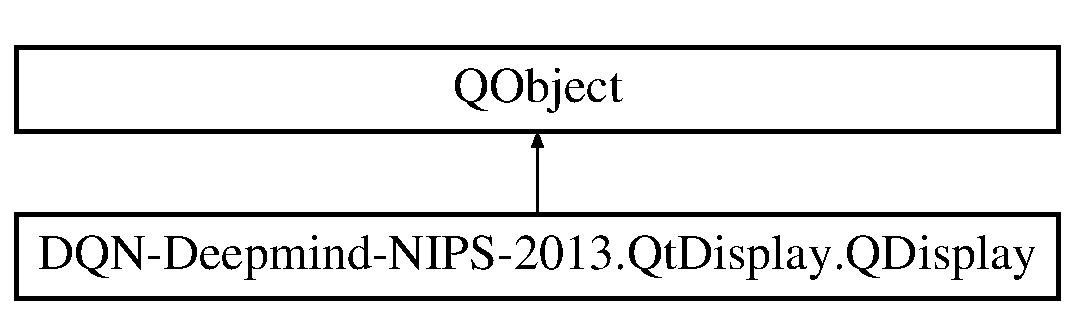
\includegraphics[height=2.000000cm]{classDQN-Deepmind-NIPS-2013_1_1QtDisplay_1_1QDisplay}
\end{center}
\end{figure}
\subsection*{Public Member Functions}
\begin{DoxyCompactItemize}
\item 
def \hyperlink{classDQN-Deepmind-NIPS-2013_1_1QtDisplay_1_1QDisplay_a4bf429fba1b45e555b41cac72f3d6f6a}{\+\_\+\+\_\+init\+\_\+\+\_\+} (self)
\begin{DoxyCompactList}\small\item\em The \hyperlink{classDQN-Deepmind-NIPS-2013_1_1QtDisplay_1_1QDisplay}{Q\+Display} constructor initializes a new \hyperlink{classDQN-Deepmind-NIPS-2013_1_1QtDisplay_1_1QDisplay}{Q\+Display} object. \end{DoxyCompactList}\item 
def \hyperlink{classDQN-Deepmind-NIPS-2013_1_1QtDisplay_1_1QDisplay_ae9c369b6776a7ca0805044f597be7cb2}{run} (self, ready)
\begin{DoxyCompactList}\small\item\em The run method initializes the object and connect the signals to their handlers. \end{DoxyCompactList}\item 
def \hyperlink{classDQN-Deepmind-NIPS-2013_1_1QtDisplay_1_1QDisplay_a12e947e8732fe3848a4746d4d3cf75c3}{initialize} (self)
\begin{DoxyCompactList}\small\item\em The initialize method initializes the application. \end{DoxyCompactList}\item 
def \hyperlink{classDQN-Deepmind-NIPS-2013_1_1QtDisplay_1_1QDisplay_ab3bca6243b3015a5bb26d0c00ba80d8f}{connect\+Signals} (self)
\begin{DoxyCompactList}\small\item\em The connect\+Signals method connects the signals to their handlers. \end{DoxyCompactList}\item 
def \hyperlink{classDQN-Deepmind-NIPS-2013_1_1QtDisplay_1_1QDisplay_adf1649fb26b3af16c155db2adf1275d2}{create\+Plotter} (self)
\begin{DoxyCompactList}\small\item\em The create\+Plotter method sends a signal to the thread that manage the display in order to ask him to create a plotter object. \end{DoxyCompactList}\item 
def \hyperlink{classDQN-Deepmind-NIPS-2013_1_1QtDisplay_1_1QDisplay_af84de3d09bc8fc27f09f5e6a3c4775a1}{create\+Env\+Display} (self, env, freq)
\begin{DoxyCompactList}\small\item\em The create\+Env\+Display method sends a signal to the thread that manage the display in order to ask him to create an \hyperlink{namespaceDQN-Deepmind-NIPS-2013_1_1EnvDisplay}{Env\+Display} object. \end{DoxyCompactList}\item 
def \hyperlink{classDQN-Deepmind-NIPS-2013_1_1QtDisplay_1_1QDisplay_aa399a47324e5e725fd5f5fd393e997ef}{plotter} (self)
\begin{DoxyCompactList}\small\item\em The plotter method wait for the plotter object to be initialized and returns the object. \end{DoxyCompactList}\item 
def \hyperlink{classDQN-Deepmind-NIPS-2013_1_1QtDisplay_1_1QDisplay_a50d2c693245a9a3f617ed2295e4d87f3}{env\+Display} (self)
\begin{DoxyCompactList}\small\item\em The env\+Display method wait for the env\+Display object to be initialized and returns the object. \end{DoxyCompactList}\item 
def \hyperlink{classDQN-Deepmind-NIPS-2013_1_1QtDisplay_1_1QDisplay_ac4d39e4b6aff27f85280f53878adee37}{exit} (self)
\begin{DoxyCompactList}\small\item\em The exit method force the event loop to quit. \end{DoxyCompactList}\end{DoxyCompactItemize}
\subsection*{Static Public Attributes}
\begin{DoxyCompactItemize}
\item 
\hyperlink{classDQN-Deepmind-NIPS-2013_1_1QtDisplay_1_1QDisplay_a9fce093a7c41ba05405ccdea20f542ad}{create\+\_\+plotter\+\_\+sig} = qtc.\+pyqt\+Signal()
\begin{DoxyCompactList}\small\item\em The create\+\_\+plotter\+\_\+sig signal signals the the thread that manages the display to create a new plotter object. \end{DoxyCompactList}\item 
\hyperlink{classDQN-Deepmind-NIPS-2013_1_1QtDisplay_1_1QDisplay_adf7d2844b0fc2026a3d4c2ed3d1218b9}{create\+\_\+env\+\_\+display\+\_\+sig} = qtc.\+pyqt\+Signal(object, int)
\begin{DoxyCompactList}\small\item\em The create\+\_\+env\+\_\+display\+\_\+sig signal signals the the thread that manages the display to create a new environment display object. \end{DoxyCompactList}\end{DoxyCompactItemize}


\subsection{Detailed Description}
The \hyperlink{classDQN-Deepmind-NIPS-2013_1_1QtDisplay_1_1QDisplay}{Q\+Display} class provides a way to integrate different window or Qt applications. 

This class is a Qt\+Core.\+Q\+Object that hold the Q\+Application and starts the event loop when the \textquotesingle{}run\textquotesingle{} method is called 

\subsection{Constructor \& Destructor Documentation}
\hypertarget{classDQN-Deepmind-NIPS-2013_1_1QtDisplay_1_1QDisplay_a4bf429fba1b45e555b41cac72f3d6f6a}{}\label{classDQN-Deepmind-NIPS-2013_1_1QtDisplay_1_1QDisplay_a4bf429fba1b45e555b41cac72f3d6f6a} 
\index{D\+Q\+N-\/\+Deepmind-\/\+N\+I\+P\+S-\/2013\+::\+Qt\+Display\+::\+Q\+Display@{D\+Q\+N-\/\+Deepmind-\/\+N\+I\+P\+S-\/2013\+::\+Qt\+Display\+::\+Q\+Display}!\+\_\+\+\_\+init\+\_\+\+\_\+@{\+\_\+\+\_\+init\+\_\+\+\_\+}}
\index{\+\_\+\+\_\+init\+\_\+\+\_\+@{\+\_\+\+\_\+init\+\_\+\+\_\+}!D\+Q\+N-\/\+Deepmind-\/\+N\+I\+P\+S-\/2013\+::\+Qt\+Display\+::\+Q\+Display@{D\+Q\+N-\/\+Deepmind-\/\+N\+I\+P\+S-\/2013\+::\+Qt\+Display\+::\+Q\+Display}}
\subsubsection{\texorpdfstring{\+\_\+\+\_\+init\+\_\+\+\_\+()}{\_\_init\_\_()}}
{\footnotesize\ttfamily def D\+QN-\/Deepmind-\/N\+I\+PS-\/2013.Qt\+Display.\+Q\+Display.\+\_\+\+\_\+init\+\_\+\+\_\+ (\begin{DoxyParamCaption}\item[{}]{self }\end{DoxyParamCaption})}



The \hyperlink{classDQN-Deepmind-NIPS-2013_1_1QtDisplay_1_1QDisplay}{Q\+Display} constructor initializes a new \hyperlink{classDQN-Deepmind-NIPS-2013_1_1QtDisplay_1_1QDisplay}{Q\+Display} object. 

There should only be one and only one \hyperlink{classDQN-Deepmind-NIPS-2013_1_1QtDisplay_1_1QDisplay}{Q\+Display} object 

\subsection{Member Function Documentation}
\hypertarget{classDQN-Deepmind-NIPS-2013_1_1QtDisplay_1_1QDisplay_ab3bca6243b3015a5bb26d0c00ba80d8f}{}\label{classDQN-Deepmind-NIPS-2013_1_1QtDisplay_1_1QDisplay_ab3bca6243b3015a5bb26d0c00ba80d8f} 
\index{D\+Q\+N-\/\+Deepmind-\/\+N\+I\+P\+S-\/2013\+::\+Qt\+Display\+::\+Q\+Display@{D\+Q\+N-\/\+Deepmind-\/\+N\+I\+P\+S-\/2013\+::\+Qt\+Display\+::\+Q\+Display}!connect\+Signals@{connect\+Signals}}
\index{connect\+Signals@{connect\+Signals}!D\+Q\+N-\/\+Deepmind-\/\+N\+I\+P\+S-\/2013\+::\+Qt\+Display\+::\+Q\+Display@{D\+Q\+N-\/\+Deepmind-\/\+N\+I\+P\+S-\/2013\+::\+Qt\+Display\+::\+Q\+Display}}
\subsubsection{\texorpdfstring{connect\+Signals()}{connectSignals()}}
{\footnotesize\ttfamily def D\+QN-\/Deepmind-\/N\+I\+PS-\/2013.Qt\+Display.\+Q\+Display.\+connect\+Signals (\begin{DoxyParamCaption}\item[{}]{self }\end{DoxyParamCaption})}



The connect\+Signals method connects the signals to their handlers. 

\hypertarget{classDQN-Deepmind-NIPS-2013_1_1QtDisplay_1_1QDisplay_af84de3d09bc8fc27f09f5e6a3c4775a1}{}\label{classDQN-Deepmind-NIPS-2013_1_1QtDisplay_1_1QDisplay_af84de3d09bc8fc27f09f5e6a3c4775a1} 
\index{D\+Q\+N-\/\+Deepmind-\/\+N\+I\+P\+S-\/2013\+::\+Qt\+Display\+::\+Q\+Display@{D\+Q\+N-\/\+Deepmind-\/\+N\+I\+P\+S-\/2013\+::\+Qt\+Display\+::\+Q\+Display}!create\+Env\+Display@{create\+Env\+Display}}
\index{create\+Env\+Display@{create\+Env\+Display}!D\+Q\+N-\/\+Deepmind-\/\+N\+I\+P\+S-\/2013\+::\+Qt\+Display\+::\+Q\+Display@{D\+Q\+N-\/\+Deepmind-\/\+N\+I\+P\+S-\/2013\+::\+Qt\+Display\+::\+Q\+Display}}
\subsubsection{\texorpdfstring{create\+Env\+Display()}{createEnvDisplay()}}
{\footnotesize\ttfamily def D\+QN-\/Deepmind-\/N\+I\+PS-\/2013.Qt\+Display.\+Q\+Display.\+create\+Env\+Display (\begin{DoxyParamCaption}\item[{}]{self,  }\item[{}]{env,  }\item[{}]{freq }\end{DoxyParamCaption})}



The create\+Env\+Display method sends a signal to the thread that manage the display in order to ask him to create an \hyperlink{namespaceDQN-Deepmind-NIPS-2013_1_1EnvDisplay}{Env\+Display} object. 

\hypertarget{classDQN-Deepmind-NIPS-2013_1_1QtDisplay_1_1QDisplay_adf1649fb26b3af16c155db2adf1275d2}{}\label{classDQN-Deepmind-NIPS-2013_1_1QtDisplay_1_1QDisplay_adf1649fb26b3af16c155db2adf1275d2} 
\index{D\+Q\+N-\/\+Deepmind-\/\+N\+I\+P\+S-\/2013\+::\+Qt\+Display\+::\+Q\+Display@{D\+Q\+N-\/\+Deepmind-\/\+N\+I\+P\+S-\/2013\+::\+Qt\+Display\+::\+Q\+Display}!create\+Plotter@{create\+Plotter}}
\index{create\+Plotter@{create\+Plotter}!D\+Q\+N-\/\+Deepmind-\/\+N\+I\+P\+S-\/2013\+::\+Qt\+Display\+::\+Q\+Display@{D\+Q\+N-\/\+Deepmind-\/\+N\+I\+P\+S-\/2013\+::\+Qt\+Display\+::\+Q\+Display}}
\subsubsection{\texorpdfstring{create\+Plotter()}{createPlotter()}}
{\footnotesize\ttfamily def D\+QN-\/Deepmind-\/N\+I\+PS-\/2013.Qt\+Display.\+Q\+Display.\+create\+Plotter (\begin{DoxyParamCaption}\item[{}]{self }\end{DoxyParamCaption})}



The create\+Plotter method sends a signal to the thread that manage the display in order to ask him to create a plotter object. 

\hypertarget{classDQN-Deepmind-NIPS-2013_1_1QtDisplay_1_1QDisplay_a50d2c693245a9a3f617ed2295e4d87f3}{}\label{classDQN-Deepmind-NIPS-2013_1_1QtDisplay_1_1QDisplay_a50d2c693245a9a3f617ed2295e4d87f3} 
\index{D\+Q\+N-\/\+Deepmind-\/\+N\+I\+P\+S-\/2013\+::\+Qt\+Display\+::\+Q\+Display@{D\+Q\+N-\/\+Deepmind-\/\+N\+I\+P\+S-\/2013\+::\+Qt\+Display\+::\+Q\+Display}!env\+Display@{env\+Display}}
\index{env\+Display@{env\+Display}!D\+Q\+N-\/\+Deepmind-\/\+N\+I\+P\+S-\/2013\+::\+Qt\+Display\+::\+Q\+Display@{D\+Q\+N-\/\+Deepmind-\/\+N\+I\+P\+S-\/2013\+::\+Qt\+Display\+::\+Q\+Display}}
\subsubsection{\texorpdfstring{env\+Display()}{envDisplay()}}
{\footnotesize\ttfamily def D\+QN-\/Deepmind-\/N\+I\+PS-\/2013.Qt\+Display.\+Q\+Display.\+env\+Display (\begin{DoxyParamCaption}\item[{}]{self }\end{DoxyParamCaption})}



The env\+Display method wait for the env\+Display object to be initialized and returns the object. 

\begin{DoxyReturn}{Returns}
A reference to the env\+Display object managed by this class 
\end{DoxyReturn}
\hypertarget{classDQN-Deepmind-NIPS-2013_1_1QtDisplay_1_1QDisplay_ac4d39e4b6aff27f85280f53878adee37}{}\label{classDQN-Deepmind-NIPS-2013_1_1QtDisplay_1_1QDisplay_ac4d39e4b6aff27f85280f53878adee37} 
\index{D\+Q\+N-\/\+Deepmind-\/\+N\+I\+P\+S-\/2013\+::\+Qt\+Display\+::\+Q\+Display@{D\+Q\+N-\/\+Deepmind-\/\+N\+I\+P\+S-\/2013\+::\+Qt\+Display\+::\+Q\+Display}!exit@{exit}}
\index{exit@{exit}!D\+Q\+N-\/\+Deepmind-\/\+N\+I\+P\+S-\/2013\+::\+Qt\+Display\+::\+Q\+Display@{D\+Q\+N-\/\+Deepmind-\/\+N\+I\+P\+S-\/2013\+::\+Qt\+Display\+::\+Q\+Display}}
\subsubsection{\texorpdfstring{exit()}{exit()}}
{\footnotesize\ttfamily def D\+QN-\/Deepmind-\/N\+I\+PS-\/2013.Qt\+Display.\+Q\+Display.\+exit (\begin{DoxyParamCaption}\item[{}]{self }\end{DoxyParamCaption})}



The exit method force the event loop to quit. 

\hypertarget{classDQN-Deepmind-NIPS-2013_1_1QtDisplay_1_1QDisplay_a12e947e8732fe3848a4746d4d3cf75c3}{}\label{classDQN-Deepmind-NIPS-2013_1_1QtDisplay_1_1QDisplay_a12e947e8732fe3848a4746d4d3cf75c3} 
\index{D\+Q\+N-\/\+Deepmind-\/\+N\+I\+P\+S-\/2013\+::\+Qt\+Display\+::\+Q\+Display@{D\+Q\+N-\/\+Deepmind-\/\+N\+I\+P\+S-\/2013\+::\+Qt\+Display\+::\+Q\+Display}!initialize@{initialize}}
\index{initialize@{initialize}!D\+Q\+N-\/\+Deepmind-\/\+N\+I\+P\+S-\/2013\+::\+Qt\+Display\+::\+Q\+Display@{D\+Q\+N-\/\+Deepmind-\/\+N\+I\+P\+S-\/2013\+::\+Qt\+Display\+::\+Q\+Display}}
\subsubsection{\texorpdfstring{initialize()}{initialize()}}
{\footnotesize\ttfamily def D\+QN-\/Deepmind-\/N\+I\+PS-\/2013.Qt\+Display.\+Q\+Display.\+initialize (\begin{DoxyParamCaption}\item[{}]{self }\end{DoxyParamCaption})}



The initialize method initializes the application. 

\hypertarget{classDQN-Deepmind-NIPS-2013_1_1QtDisplay_1_1QDisplay_aa399a47324e5e725fd5f5fd393e997ef}{}\label{classDQN-Deepmind-NIPS-2013_1_1QtDisplay_1_1QDisplay_aa399a47324e5e725fd5f5fd393e997ef} 
\index{D\+Q\+N-\/\+Deepmind-\/\+N\+I\+P\+S-\/2013\+::\+Qt\+Display\+::\+Q\+Display@{D\+Q\+N-\/\+Deepmind-\/\+N\+I\+P\+S-\/2013\+::\+Qt\+Display\+::\+Q\+Display}!plotter@{plotter}}
\index{plotter@{plotter}!D\+Q\+N-\/\+Deepmind-\/\+N\+I\+P\+S-\/2013\+::\+Qt\+Display\+::\+Q\+Display@{D\+Q\+N-\/\+Deepmind-\/\+N\+I\+P\+S-\/2013\+::\+Qt\+Display\+::\+Q\+Display}}
\subsubsection{\texorpdfstring{plotter()}{plotter()}}
{\footnotesize\ttfamily def D\+QN-\/Deepmind-\/N\+I\+PS-\/2013.Qt\+Display.\+Q\+Display.\+plotter (\begin{DoxyParamCaption}\item[{}]{self }\end{DoxyParamCaption})}



The plotter method wait for the plotter object to be initialized and returns the object. 

\begin{DoxyReturn}{Returns}
A reference to the plotter object managed by this class 
\end{DoxyReturn}
\hypertarget{classDQN-Deepmind-NIPS-2013_1_1QtDisplay_1_1QDisplay_ae9c369b6776a7ca0805044f597be7cb2}{}\label{classDQN-Deepmind-NIPS-2013_1_1QtDisplay_1_1QDisplay_ae9c369b6776a7ca0805044f597be7cb2} 
\index{D\+Q\+N-\/\+Deepmind-\/\+N\+I\+P\+S-\/2013\+::\+Qt\+Display\+::\+Q\+Display@{D\+Q\+N-\/\+Deepmind-\/\+N\+I\+P\+S-\/2013\+::\+Qt\+Display\+::\+Q\+Display}!run@{run}}
\index{run@{run}!D\+Q\+N-\/\+Deepmind-\/\+N\+I\+P\+S-\/2013\+::\+Qt\+Display\+::\+Q\+Display@{D\+Q\+N-\/\+Deepmind-\/\+N\+I\+P\+S-\/2013\+::\+Qt\+Display\+::\+Q\+Display}}
\subsubsection{\texorpdfstring{run()}{run()}}
{\footnotesize\ttfamily def D\+QN-\/Deepmind-\/N\+I\+PS-\/2013.Qt\+Display.\+Q\+Display.\+run (\begin{DoxyParamCaption}\item[{}]{self,  }\item[{}]{ready }\end{DoxyParamCaption})}



The run method initializes the object and connect the signals to their handlers. 

Then, it set the given event and start the event loop


\begin{DoxyParams}{Parameters}
{\em ready} & \+: A threading.\+Event object that will be set after the signals are connected \\
\hline
\end{DoxyParams}


\subsection{Member Data Documentation}
\hypertarget{classDQN-Deepmind-NIPS-2013_1_1QtDisplay_1_1QDisplay_adf7d2844b0fc2026a3d4c2ed3d1218b9}{}\label{classDQN-Deepmind-NIPS-2013_1_1QtDisplay_1_1QDisplay_adf7d2844b0fc2026a3d4c2ed3d1218b9} 
\index{D\+Q\+N-\/\+Deepmind-\/\+N\+I\+P\+S-\/2013\+::\+Qt\+Display\+::\+Q\+Display@{D\+Q\+N-\/\+Deepmind-\/\+N\+I\+P\+S-\/2013\+::\+Qt\+Display\+::\+Q\+Display}!create\+\_\+env\+\_\+display\+\_\+sig@{create\+\_\+env\+\_\+display\+\_\+sig}}
\index{create\+\_\+env\+\_\+display\+\_\+sig@{create\+\_\+env\+\_\+display\+\_\+sig}!D\+Q\+N-\/\+Deepmind-\/\+N\+I\+P\+S-\/2013\+::\+Qt\+Display\+::\+Q\+Display@{D\+Q\+N-\/\+Deepmind-\/\+N\+I\+P\+S-\/2013\+::\+Qt\+Display\+::\+Q\+Display}}
\subsubsection{\texorpdfstring{create\+\_\+env\+\_\+display\+\_\+sig}{create\_env\_display\_sig}}
{\footnotesize\ttfamily D\+QN-\/Deepmind-\/N\+I\+PS-\/2013.Qt\+Display.\+Q\+Display.\+create\+\_\+env\+\_\+display\+\_\+sig = qtc.\+pyqt\+Signal(object, int)\hspace{0.3cm}{\ttfamily [static]}}



The create\+\_\+env\+\_\+display\+\_\+sig signal signals the the thread that manages the display to create a new environment display object. 

\hypertarget{classDQN-Deepmind-NIPS-2013_1_1QtDisplay_1_1QDisplay_a9fce093a7c41ba05405ccdea20f542ad}{}\label{classDQN-Deepmind-NIPS-2013_1_1QtDisplay_1_1QDisplay_a9fce093a7c41ba05405ccdea20f542ad} 
\index{D\+Q\+N-\/\+Deepmind-\/\+N\+I\+P\+S-\/2013\+::\+Qt\+Display\+::\+Q\+Display@{D\+Q\+N-\/\+Deepmind-\/\+N\+I\+P\+S-\/2013\+::\+Qt\+Display\+::\+Q\+Display}!create\+\_\+plotter\+\_\+sig@{create\+\_\+plotter\+\_\+sig}}
\index{create\+\_\+plotter\+\_\+sig@{create\+\_\+plotter\+\_\+sig}!D\+Q\+N-\/\+Deepmind-\/\+N\+I\+P\+S-\/2013\+::\+Qt\+Display\+::\+Q\+Display@{D\+Q\+N-\/\+Deepmind-\/\+N\+I\+P\+S-\/2013\+::\+Qt\+Display\+::\+Q\+Display}}
\subsubsection{\texorpdfstring{create\+\_\+plotter\+\_\+sig}{create\_plotter\_sig}}
{\footnotesize\ttfamily D\+QN-\/Deepmind-\/N\+I\+PS-\/2013.Qt\+Display.\+Q\+Display.\+create\+\_\+plotter\+\_\+sig = qtc.\+pyqt\+Signal()\hspace{0.3cm}{\ttfamily [static]}}



The create\+\_\+plotter\+\_\+sig signal signals the the thread that manages the display to create a new plotter object. 



The documentation for this class was generated from the following file\+:\begin{DoxyCompactItemize}
\item 
\hyperlink{QtDisplay_8py}{Qt\+Display.\+py}\end{DoxyCompactItemize}

\hypertarget{classDQN-Deepmind-NIPS-2013_1_1agent_1_1DeepMindAgent_1_1ReplayMemory}{}\section{D\+Q\+N-\/\+Deepmind-\/\+N\+I\+P\+S-\/2013.agent.\+Deep\+Mind\+Agent.\+Replay\+Memory Class Reference}
\label{classDQN-Deepmind-NIPS-2013_1_1agent_1_1DeepMindAgent_1_1ReplayMemory}\index{D\+Q\+N-\/\+Deepmind-\/\+N\+I\+P\+S-\/2013.\+agent.\+Deep\+Mind\+Agent.\+Replay\+Memory@{D\+Q\+N-\/\+Deepmind-\/\+N\+I\+P\+S-\/2013.\+agent.\+Deep\+Mind\+Agent.\+Replay\+Memory}}


The \hyperlink{classDQN-Deepmind-NIPS-2013_1_1agent_1_1DeepMindAgent_1_1ReplayMemory}{Replay\+Memory} class is a list of past experiences as defined in the paper \href{https://www.cs.toronto.edu/~vmnih/docs/dqn.pdf}{\tt Playing Atari with Deep Reinforcement Learning}  


\subsection*{Public Member Functions}
\begin{DoxyCompactItemize}
\item 
def \hyperlink{classDQN-Deepmind-NIPS-2013_1_1agent_1_1DeepMindAgent_1_1ReplayMemory_a8b43f49e7cc41952febfe6bdf7003a83}{\+\_\+\+\_\+init\+\_\+\+\_\+} (self, capacity, act\+Cnt, c, h, w)
\begin{DoxyCompactList}\small\item\em The \hyperlink{classDQN-Deepmind-NIPS-2013_1_1agent_1_1DeepMindAgent_1_1ReplayMemory}{Replay\+Memory} constructor initializes a \hyperlink{classDQN-Deepmind-NIPS-2013_1_1agent_1_1DeepMindAgent_1_1ReplayMemory}{Replay\+Memory} of the given capacity. \end{DoxyCompactList}\item 
def \hyperlink{classDQN-Deepmind-NIPS-2013_1_1agent_1_1DeepMindAgent_1_1ReplayMemory_aef90d1c859c72ea6de32ed97cf0f4a7c}{\+\_\+\+\_\+len\+\_\+\+\_\+} (self)
\begin{DoxyCompactList}\small\item\em The {\bfseries len} method returns the number of experiences stored in the replay memory. \end{DoxyCompactList}\item 
def \hyperlink{classDQN-Deepmind-NIPS-2013_1_1agent_1_1DeepMindAgent_1_1ReplayMemory_ab920b49aedb6569d214cf0e6fd390cea}{add\+Images} (self, imgs)
\begin{DoxyCompactList}\small\item\em The add\+Images method adds the given images to the image set. \end{DoxyCompactList}\item 
def \hyperlink{classDQN-Deepmind-NIPS-2013_1_1agent_1_1DeepMindAgent_1_1ReplayMemory_ab43dd0161bc7e1dc749a6188062880fa}{add\+Experience} (self, img, a, r, t)
\begin{DoxyCompactList}\small\item\em Adds the given experience to the replay memory. \end{DoxyCompactList}\item 
def \hyperlink{classDQN-Deepmind-NIPS-2013_1_1agent_1_1DeepMindAgent_1_1ReplayMemory_a345939d730803f20978861c2ba6cd397}{minibatch} (self, size)
\begin{DoxyCompactList}\small\item\em The minibatch method returns a random minibatch which size is the minimum between the given size and the size of the replay memory. \end{DoxyCompactList}\end{DoxyCompactItemize}


\subsection{Detailed Description}
The \hyperlink{classDQN-Deepmind-NIPS-2013_1_1agent_1_1DeepMindAgent_1_1ReplayMemory}{Replay\+Memory} class is a list of past experiences as defined in the paper \href{https://www.cs.toronto.edu/~vmnih/docs/dqn.pdf}{\tt Playing Atari with Deep Reinforcement Learning} 

The replay memory is made of an Image\+Set that will keep given images in memory. If \textquotesingle{}c\textquotesingle{} is the number of images a state is made of, the replay memory keeps the ids of the \textquotesingle{}c\textquotesingle{} last inserted images. Then when a new experience is inserted into the replay memory, only one image has to be given. The replay memory assumes that the initial state related to this experience is made of the \textquotesingle{}c\textquotesingle{} last images and that the terminal state of this experience is made of the \textquotesingle{}c-\/1\textquotesingle{} last inserted images plus the new given image. 

\subsection{Constructor \& Destructor Documentation}
\hypertarget{classDQN-Deepmind-NIPS-2013_1_1agent_1_1DeepMindAgent_1_1ReplayMemory_a8b43f49e7cc41952febfe6bdf7003a83}{}\label{classDQN-Deepmind-NIPS-2013_1_1agent_1_1DeepMindAgent_1_1ReplayMemory_a8b43f49e7cc41952febfe6bdf7003a83} 
\index{D\+Q\+N-\/\+Deepmind-\/\+N\+I\+P\+S-\/2013\+::agent\+::\+Deep\+Mind\+Agent\+::\+Replay\+Memory@{D\+Q\+N-\/\+Deepmind-\/\+N\+I\+P\+S-\/2013\+::agent\+::\+Deep\+Mind\+Agent\+::\+Replay\+Memory}!\+\_\+\+\_\+init\+\_\+\+\_\+@{\+\_\+\+\_\+init\+\_\+\+\_\+}}
\index{\+\_\+\+\_\+init\+\_\+\+\_\+@{\+\_\+\+\_\+init\+\_\+\+\_\+}!D\+Q\+N-\/\+Deepmind-\/\+N\+I\+P\+S-\/2013\+::agent\+::\+Deep\+Mind\+Agent\+::\+Replay\+Memory@{D\+Q\+N-\/\+Deepmind-\/\+N\+I\+P\+S-\/2013\+::agent\+::\+Deep\+Mind\+Agent\+::\+Replay\+Memory}}
\subsubsection{\texorpdfstring{\+\_\+\+\_\+init\+\_\+\+\_\+()}{\_\_init\_\_()}}
{\footnotesize\ttfamily def D\+QN-\/Deepmind-\/N\+I\+PS-\/2013.agent.\+Deep\+Mind\+Agent.\+Replay\+Memory.\+\_\+\+\_\+init\+\_\+\+\_\+ (\begin{DoxyParamCaption}\item[{}]{self,  }\item[{}]{capacity,  }\item[{}]{act\+Cnt,  }\item[{}]{c,  }\item[{}]{h,  }\item[{}]{w }\end{DoxyParamCaption})}



The \hyperlink{classDQN-Deepmind-NIPS-2013_1_1agent_1_1DeepMindAgent_1_1ReplayMemory}{Replay\+Memory} constructor initializes a \hyperlink{classDQN-Deepmind-NIPS-2013_1_1agent_1_1DeepMindAgent_1_1ReplayMemory}{Replay\+Memory} of the given capacity. 


\begin{DoxyParams}{Parameters}
{\em capacity} & \+: The number of elements the replay memory is able to store before erasing its oldest inserted element to insert new ones \\
\hline
{\em c} & \+: The number of channels (i.\+e. images) per sequence \\
\hline
{\em h} & \+: The heights of an images \\
\hline
{\em w} & \+: The width of an image \\
\hline
{\em act\+Cnt} & \+: The number of possible actions \\
\hline
\end{DoxyParams}


\subsection{Member Function Documentation}
\hypertarget{classDQN-Deepmind-NIPS-2013_1_1agent_1_1DeepMindAgent_1_1ReplayMemory_aef90d1c859c72ea6de32ed97cf0f4a7c}{}\label{classDQN-Deepmind-NIPS-2013_1_1agent_1_1DeepMindAgent_1_1ReplayMemory_aef90d1c859c72ea6de32ed97cf0f4a7c} 
\index{D\+Q\+N-\/\+Deepmind-\/\+N\+I\+P\+S-\/2013\+::agent\+::\+Deep\+Mind\+Agent\+::\+Replay\+Memory@{D\+Q\+N-\/\+Deepmind-\/\+N\+I\+P\+S-\/2013\+::agent\+::\+Deep\+Mind\+Agent\+::\+Replay\+Memory}!\+\_\+\+\_\+len\+\_\+\+\_\+@{\+\_\+\+\_\+len\+\_\+\+\_\+}}
\index{\+\_\+\+\_\+len\+\_\+\+\_\+@{\+\_\+\+\_\+len\+\_\+\+\_\+}!D\+Q\+N-\/\+Deepmind-\/\+N\+I\+P\+S-\/2013\+::agent\+::\+Deep\+Mind\+Agent\+::\+Replay\+Memory@{D\+Q\+N-\/\+Deepmind-\/\+N\+I\+P\+S-\/2013\+::agent\+::\+Deep\+Mind\+Agent\+::\+Replay\+Memory}}
\subsubsection{\texorpdfstring{\+\_\+\+\_\+len\+\_\+\+\_\+()}{\_\_len\_\_()}}
{\footnotesize\ttfamily def D\+QN-\/Deepmind-\/N\+I\+PS-\/2013.agent.\+Deep\+Mind\+Agent.\+Replay\+Memory.\+\_\+\+\_\+len\+\_\+\+\_\+ (\begin{DoxyParamCaption}\item[{}]{self }\end{DoxyParamCaption})}



The {\bfseries len} method returns the number of experiences stored in the replay memory. 

\hypertarget{classDQN-Deepmind-NIPS-2013_1_1agent_1_1DeepMindAgent_1_1ReplayMemory_ab43dd0161bc7e1dc749a6188062880fa}{}\label{classDQN-Deepmind-NIPS-2013_1_1agent_1_1DeepMindAgent_1_1ReplayMemory_ab43dd0161bc7e1dc749a6188062880fa} 
\index{D\+Q\+N-\/\+Deepmind-\/\+N\+I\+P\+S-\/2013\+::agent\+::\+Deep\+Mind\+Agent\+::\+Replay\+Memory@{D\+Q\+N-\/\+Deepmind-\/\+N\+I\+P\+S-\/2013\+::agent\+::\+Deep\+Mind\+Agent\+::\+Replay\+Memory}!add\+Experience@{add\+Experience}}
\index{add\+Experience@{add\+Experience}!D\+Q\+N-\/\+Deepmind-\/\+N\+I\+P\+S-\/2013\+::agent\+::\+Deep\+Mind\+Agent\+::\+Replay\+Memory@{D\+Q\+N-\/\+Deepmind-\/\+N\+I\+P\+S-\/2013\+::agent\+::\+Deep\+Mind\+Agent\+::\+Replay\+Memory}}
\subsubsection{\texorpdfstring{add\+Experience()}{addExperience()}}
{\footnotesize\ttfamily def D\+QN-\/Deepmind-\/N\+I\+PS-\/2013.agent.\+Deep\+Mind\+Agent.\+Replay\+Memory.\+add\+Experience (\begin{DoxyParamCaption}\item[{}]{self,  }\item[{}]{img,  }\item[{}]{a,  }\item[{}]{r,  }\item[{}]{t }\end{DoxyParamCaption})}



Adds the given experience to the replay memory. 


\begin{DoxyParams}{Parameters}
{\em img} & \+: The new image to add to the image set \\
\hline
{\em a} & \+: The id of the last action taken \\
\hline
{\em r} & \+: The last reward perceived \\
\hline
{\em t} & \+: Wheter the reached state is a terminal state or not \\
\hline
\end{DoxyParams}
\hypertarget{classDQN-Deepmind-NIPS-2013_1_1agent_1_1DeepMindAgent_1_1ReplayMemory_ab920b49aedb6569d214cf0e6fd390cea}{}\label{classDQN-Deepmind-NIPS-2013_1_1agent_1_1DeepMindAgent_1_1ReplayMemory_ab920b49aedb6569d214cf0e6fd390cea} 
\index{D\+Q\+N-\/\+Deepmind-\/\+N\+I\+P\+S-\/2013\+::agent\+::\+Deep\+Mind\+Agent\+::\+Replay\+Memory@{D\+Q\+N-\/\+Deepmind-\/\+N\+I\+P\+S-\/2013\+::agent\+::\+Deep\+Mind\+Agent\+::\+Replay\+Memory}!add\+Images@{add\+Images}}
\index{add\+Images@{add\+Images}!D\+Q\+N-\/\+Deepmind-\/\+N\+I\+P\+S-\/2013\+::agent\+::\+Deep\+Mind\+Agent\+::\+Replay\+Memory@{D\+Q\+N-\/\+Deepmind-\/\+N\+I\+P\+S-\/2013\+::agent\+::\+Deep\+Mind\+Agent\+::\+Replay\+Memory}}
\subsubsection{\texorpdfstring{add\+Images()}{addImages()}}
{\footnotesize\ttfamily def D\+QN-\/Deepmind-\/N\+I\+PS-\/2013.agent.\+Deep\+Mind\+Agent.\+Replay\+Memory.\+add\+Images (\begin{DoxyParamCaption}\item[{}]{self,  }\item[{}]{imgs }\end{DoxyParamCaption})}



The add\+Images method adds the given images to the image set. 


\begin{DoxyParams}{Parameters}
{\em imgs} & \+: A list of the images to add to the set \\
\hline
\end{DoxyParams}
\hypertarget{classDQN-Deepmind-NIPS-2013_1_1agent_1_1DeepMindAgent_1_1ReplayMemory_a345939d730803f20978861c2ba6cd397}{}\label{classDQN-Deepmind-NIPS-2013_1_1agent_1_1DeepMindAgent_1_1ReplayMemory_a345939d730803f20978861c2ba6cd397} 
\index{D\+Q\+N-\/\+Deepmind-\/\+N\+I\+P\+S-\/2013\+::agent\+::\+Deep\+Mind\+Agent\+::\+Replay\+Memory@{D\+Q\+N-\/\+Deepmind-\/\+N\+I\+P\+S-\/2013\+::agent\+::\+Deep\+Mind\+Agent\+::\+Replay\+Memory}!minibatch@{minibatch}}
\index{minibatch@{minibatch}!D\+Q\+N-\/\+Deepmind-\/\+N\+I\+P\+S-\/2013\+::agent\+::\+Deep\+Mind\+Agent\+::\+Replay\+Memory@{D\+Q\+N-\/\+Deepmind-\/\+N\+I\+P\+S-\/2013\+::agent\+::\+Deep\+Mind\+Agent\+::\+Replay\+Memory}}
\subsubsection{\texorpdfstring{minibatch()}{minibatch()}}
{\footnotesize\ttfamily def D\+QN-\/Deepmind-\/N\+I\+PS-\/2013.agent.\+Deep\+Mind\+Agent.\+Replay\+Memory.\+minibatch (\begin{DoxyParamCaption}\item[{}]{self,  }\item[{}]{size }\end{DoxyParamCaption})}



The minibatch method returns a random minibatch which size is the minimum between the given size and the size of the replay memory. 

If the replay memory is empty, the method returns None


\begin{DoxyParams}{Parameters}
{\em size} & \+: The size of the minibatch to return\\
\hline
\end{DoxyParams}
\begin{DoxyReturn}{Returns}
This method returns None if the replay memory is empty. Otherwise it returns a minibatch made of n sample drawn from the set of stored experiences, where \textquotesingle{}n\textquotesingle{} is the minimum between the length of the replay memory and the given size. The returned minibatch is a tuple which elements are the following\+:
\begin{DoxyItemize}
\item s\+\_\+t \+: an array of shape \mbox{[}n, c, h, w\mbox{]} which contains the n initial states of the minibatch
\item s\+\_\+t1 \+: an array of the shape \mbox{[}n, c, h, w\mbox{]} which contains the n states reached from respectively the n states stored in s\+\_\+t
\item a\+\_\+t \+: an array of shape \mbox{[}n, act\+Cnt\mbox{]} where every row is full of 0 except for the value at the id corresponding to the action take in the respective n states s\+\_\+t, which is then 1
\item r\+\_\+t \+: an array of shape \mbox{[}n\mbox{]} which entries are the rewards perceived while going from the n respective states s\+\_\+t to the n respective states s\+\_\+t1
\item t \+: an array of shape \mbox{[}n\mbox{]} which entries indicate if the n respective states s\+\_\+t1 are terminals or not 
\end{DoxyItemize}
\end{DoxyReturn}


The documentation for this class was generated from the following file\+:\begin{DoxyCompactItemize}
\item 
agent/\hyperlink{DeepMindAgent_8py}{Deep\+Mind\+Agent.\+py}\end{DoxyCompactItemize}

\hypertarget{classDQN-Deepmind-NIPS-2013_1_1Saver_1_1Saver}{}\section{D\+Q\+N-\/\+Deepmind-\/\+N\+I\+P\+S-\/2013.Saver.\+Saver Class Reference}
\label{classDQN-Deepmind-NIPS-2013_1_1Saver_1_1Saver}\index{D\+Q\+N-\/\+Deepmind-\/\+N\+I\+P\+S-\/2013.\+Saver.\+Saver@{D\+Q\+N-\/\+Deepmind-\/\+N\+I\+P\+S-\/2013.\+Saver.\+Saver}}


The \hyperlink{classDQN-Deepmind-NIPS-2013_1_1Saver_1_1Saver}{Saver} class provides an easy way to save or load, an agent, its network and statistics about its performances.  


\subsection*{Public Member Functions}
\begin{DoxyCompactItemize}
\item 
def \hyperlink{classDQN-Deepmind-NIPS-2013_1_1Saver_1_1Saver_ac1c5a74d16e09f25b884196bda20f70a}{\+\_\+\+\_\+init\+\_\+\+\_\+} (self, db\+Path)
\begin{DoxyCompactList}\small\item\em The \hyperlink{classDQN-Deepmind-NIPS-2013_1_1Saver_1_1Saver}{Saver} class constructor initialize the \hyperlink{classDQN-Deepmind-NIPS-2013_1_1Saver_1_1Saver}{Saver} object. \end{DoxyCompactList}\item 
def \hyperlink{classDQN-Deepmind-NIPS-2013_1_1Saver_1_1Saver_a4f61e8fbd52eef88616ef8e9ef0fab2b}{list\+Agents} (self)
\begin{DoxyCompactList}\small\item\em The list\+Agents query the database and returns a list of tuples representing the available agents. \end{DoxyCompactList}\item 
def \hyperlink{classDQN-Deepmind-NIPS-2013_1_1Saver_1_1Saver_a8deee83c5bcdd58d10abc7dadeb8d153}{list\+Networks} (self, agent\+Id)
\begin{DoxyCompactList}\small\item\em The list\+Networks method returns a list all the network availables for the given agent. \end{DoxyCompactList}\item 
def \hyperlink{classDQN-Deepmind-NIPS-2013_1_1Saver_1_1Saver_a47c6eac5868ed0525a258211a4d75cd9}{list\+Datasets} (self, shape, min\+Size, max\+Size)
\begin{DoxyCompactList}\small\item\em The list\+Datasets method returns a list of the datasets matching the given shape and which length is between the given sizes. \end{DoxyCompactList}\item 
def \hyperlink{classDQN-Deepmind-NIPS-2013_1_1Saver_1_1Saver_a21a3603e2a8e8d12d60a2640b224b952}{new\+Agent} (self, name, agent\+Type, params)
\begin{DoxyCompactList}\small\item\em The new\+Agent method records a new agent in the database. \end{DoxyCompactList}\item 
def \hyperlink{classDQN-Deepmind-NIPS-2013_1_1Saver_1_1Saver_aa0d2a62b7e514dc527745f846924e70e}{save\+Agent} (self, agent\+Id, params)
\begin{DoxyCompactList}\small\item\em The save\+Agent methods overwrites the parameters recorder for the given agent. \end{DoxyCompactList}\item 
def \hyperlink{classDQN-Deepmind-NIPS-2013_1_1Saver_1_1Saver_aebf1fa14b77298919410191ecbab6fe5}{save\+Network} (self, agent\+Id, info, network)
\begin{DoxyCompactList}\small\item\em The save\+Network method adds the given network to the list of the networks available for the given agent. \end{DoxyCompactList}\item 
def \hyperlink{classDQN-Deepmind-NIPS-2013_1_1Saver_1_1Saver_ae1370bef68104eb715e1387d69bb7cf1}{save\+Stat} (self, agent\+Id, network\+Id, name, epoch, value)
\begin{DoxyCompactList}\small\item\em The save\+Stat method saves the given statistics into the database. \end{DoxyCompactList}\item 
def \hyperlink{classDQN-Deepmind-NIPS-2013_1_1Saver_1_1Saver_a5c4872622dfd891849a22e447ec7d902}{new\+Dataset} (self, length, shape, data)
\begin{DoxyCompactList}\small\item\em The new\+Dataset method save a new dataset into the database. \end{DoxyCompactList}\item 
def \hyperlink{classDQN-Deepmind-NIPS-2013_1_1Saver_1_1Saver_aaf903c7b667b1909a17beb60c13f2398}{load\+Agent} (self, agent\+Id)
\begin{DoxyCompactList}\small\item\em The load\+Agent method returns the parameters associated to the given agent. \end{DoxyCompactList}\item 
def \hyperlink{classDQN-Deepmind-NIPS-2013_1_1Saver_1_1Saver_a90f2e74db8a2b69b94959945ffb896f6}{load\+Network} (self, agent\+Id, network\+Id=None)
\begin{DoxyCompactList}\small\item\em The load\+Network method returns the desired network. \end{DoxyCompactList}\item 
def \hyperlink{classDQN-Deepmind-NIPS-2013_1_1Saver_1_1Saver_aad377d9e28499a19a591d080e6a0df63}{load\+Network\+Epoch} (self, agent\+Id, epoch)
\begin{DoxyCompactList}\small\item\em The load\+Network\+Epoch returns the id of the network linked to the stat recorded for the given agent at the given epoch. \end{DoxyCompactList}\item 
def \hyperlink{classDQN-Deepmind-NIPS-2013_1_1Saver_1_1Saver_a76d60329698faf415c4ed0dae362f53e}{load\+Dataset} (self, set\+Id)
\begin{DoxyCompactList}\small\item\em The load\+Dataset method return the desired dataset. \end{DoxyCompactList}\end{DoxyCompactItemize}
\subsection*{Static Public Attributes}
\begin{DoxyCompactItemize}
\item 
string \hyperlink{classDQN-Deepmind-NIPS-2013_1_1Saver_1_1Saver_ab44237c14a7cc898a5952c42bb1fbfe0}{D\+E\+E\+P\+\_\+\+M\+I\+N\+D\+\_\+\+A\+G\+E\+NT} = \char`\"{}Deep\+Mind\+Agent\char`\"{}
\begin{DoxyCompactList}\small\item\em Type for an agent implementing the algorithm developped by deepmind in their paper of 2013. \end{DoxyCompactList}\end{DoxyCompactItemize}


\subsection{Detailed Description}
The \hyperlink{classDQN-Deepmind-NIPS-2013_1_1Saver_1_1Saver}{Saver} class provides an easy way to save or load, an agent, its network and statistics about its performances. 

\subsection{Constructor \& Destructor Documentation}
\hypertarget{classDQN-Deepmind-NIPS-2013_1_1Saver_1_1Saver_ac1c5a74d16e09f25b884196bda20f70a}{}\label{classDQN-Deepmind-NIPS-2013_1_1Saver_1_1Saver_ac1c5a74d16e09f25b884196bda20f70a} 
\index{D\+Q\+N-\/\+Deepmind-\/\+N\+I\+P\+S-\/2013\+::\+Saver\+::\+Saver@{D\+Q\+N-\/\+Deepmind-\/\+N\+I\+P\+S-\/2013\+::\+Saver\+::\+Saver}!\+\_\+\+\_\+init\+\_\+\+\_\+@{\+\_\+\+\_\+init\+\_\+\+\_\+}}
\index{\+\_\+\+\_\+init\+\_\+\+\_\+@{\+\_\+\+\_\+init\+\_\+\+\_\+}!D\+Q\+N-\/\+Deepmind-\/\+N\+I\+P\+S-\/2013\+::\+Saver\+::\+Saver@{D\+Q\+N-\/\+Deepmind-\/\+N\+I\+P\+S-\/2013\+::\+Saver\+::\+Saver}}
\subsubsection{\texorpdfstring{\+\_\+\+\_\+init\+\_\+\+\_\+()}{\_\_init\_\_()}}
{\footnotesize\ttfamily def D\+QN-\/Deepmind-\/N\+I\+PS-\/2013.Saver.\+Saver.\+\_\+\+\_\+init\+\_\+\+\_\+ (\begin{DoxyParamCaption}\item[{}]{self,  }\item[{}]{db\+Path }\end{DoxyParamCaption})}



The \hyperlink{classDQN-Deepmind-NIPS-2013_1_1Saver_1_1Saver}{Saver} class constructor initialize the \hyperlink{classDQN-Deepmind-NIPS-2013_1_1Saver_1_1Saver}{Saver} object. 

The constructor connects to or creates the sqlite database to use and creates the tables it needs if its required.


\begin{DoxyParams}{Parameters}
{\em db\+Path} & \+: The path to the database to connect to or to create \\
\hline
\end{DoxyParams}


\subsection{Member Function Documentation}
\hypertarget{classDQN-Deepmind-NIPS-2013_1_1Saver_1_1Saver_a4f61e8fbd52eef88616ef8e9ef0fab2b}{}\label{classDQN-Deepmind-NIPS-2013_1_1Saver_1_1Saver_a4f61e8fbd52eef88616ef8e9ef0fab2b} 
\index{D\+Q\+N-\/\+Deepmind-\/\+N\+I\+P\+S-\/2013\+::\+Saver\+::\+Saver@{D\+Q\+N-\/\+Deepmind-\/\+N\+I\+P\+S-\/2013\+::\+Saver\+::\+Saver}!list\+Agents@{list\+Agents}}
\index{list\+Agents@{list\+Agents}!D\+Q\+N-\/\+Deepmind-\/\+N\+I\+P\+S-\/2013\+::\+Saver\+::\+Saver@{D\+Q\+N-\/\+Deepmind-\/\+N\+I\+P\+S-\/2013\+::\+Saver\+::\+Saver}}
\subsubsection{\texorpdfstring{list\+Agents()}{listAgents()}}
{\footnotesize\ttfamily def D\+QN-\/Deepmind-\/N\+I\+PS-\/2013.Saver.\+Saver.\+list\+Agents (\begin{DoxyParamCaption}\item[{}]{self }\end{DoxyParamCaption})}



The list\+Agents query the database and returns a list of tuples representing the available agents. 

\begin{DoxyReturn}{Returns}
A list of tuples with agent\textquotesingle{}s attributes \+: (id, name, type, creation time stamp, parameters) 
\end{DoxyReturn}
\hypertarget{classDQN-Deepmind-NIPS-2013_1_1Saver_1_1Saver_a47c6eac5868ed0525a258211a4d75cd9}{}\label{classDQN-Deepmind-NIPS-2013_1_1Saver_1_1Saver_a47c6eac5868ed0525a258211a4d75cd9} 
\index{D\+Q\+N-\/\+Deepmind-\/\+N\+I\+P\+S-\/2013\+::\+Saver\+::\+Saver@{D\+Q\+N-\/\+Deepmind-\/\+N\+I\+P\+S-\/2013\+::\+Saver\+::\+Saver}!list\+Datasets@{list\+Datasets}}
\index{list\+Datasets@{list\+Datasets}!D\+Q\+N-\/\+Deepmind-\/\+N\+I\+P\+S-\/2013\+::\+Saver\+::\+Saver@{D\+Q\+N-\/\+Deepmind-\/\+N\+I\+P\+S-\/2013\+::\+Saver\+::\+Saver}}
\subsubsection{\texorpdfstring{list\+Datasets()}{listDatasets()}}
{\footnotesize\ttfamily def D\+QN-\/Deepmind-\/N\+I\+PS-\/2013.Saver.\+Saver.\+list\+Datasets (\begin{DoxyParamCaption}\item[{}]{self,  }\item[{}]{shape,  }\item[{}]{min\+Size,  }\item[{}]{max\+Size }\end{DoxyParamCaption})}



The list\+Datasets method returns a list of the datasets matching the given shape and which length is between the given sizes. 


\begin{DoxyParams}{Parameters}
{\em shape} & \+: The shape of the desired data set \\
\hline
{\em min\+Size} & \+: The minimum number of elements in the dataset \\
\hline
{\em max\+Size} & \+: The maximum number of elements in the dataset\\
\hline
\end{DoxyParams}
\begin{DoxyReturn}{Returns}
A list of tuples containing the id and the size of the available datasets (id, size) 
\end{DoxyReturn}
\hypertarget{classDQN-Deepmind-NIPS-2013_1_1Saver_1_1Saver_a8deee83c5bcdd58d10abc7dadeb8d153}{}\label{classDQN-Deepmind-NIPS-2013_1_1Saver_1_1Saver_a8deee83c5bcdd58d10abc7dadeb8d153} 
\index{D\+Q\+N-\/\+Deepmind-\/\+N\+I\+P\+S-\/2013\+::\+Saver\+::\+Saver@{D\+Q\+N-\/\+Deepmind-\/\+N\+I\+P\+S-\/2013\+::\+Saver\+::\+Saver}!list\+Networks@{list\+Networks}}
\index{list\+Networks@{list\+Networks}!D\+Q\+N-\/\+Deepmind-\/\+N\+I\+P\+S-\/2013\+::\+Saver\+::\+Saver@{D\+Q\+N-\/\+Deepmind-\/\+N\+I\+P\+S-\/2013\+::\+Saver\+::\+Saver}}
\subsubsection{\texorpdfstring{list\+Networks()}{listNetworks()}}
{\footnotesize\ttfamily def D\+QN-\/Deepmind-\/N\+I\+PS-\/2013.Saver.\+Saver.\+list\+Networks (\begin{DoxyParamCaption}\item[{}]{self,  }\item[{}]{agent\+Id }\end{DoxyParamCaption})}



The list\+Networks method returns a list all the network availables for the given agent. 


\begin{DoxyParams}{Parameters}
{\em agent\+Id} & \+: The id of the agent\\
\hline
\end{DoxyParams}
\begin{DoxyReturn}{Returns}
A list of tuples with the parameters of the available networks (id, agent\textquotesingle{}s id, informations, creation timestamp, network) 
\end{DoxyReturn}
\hypertarget{classDQN-Deepmind-NIPS-2013_1_1Saver_1_1Saver_aaf903c7b667b1909a17beb60c13f2398}{}\label{classDQN-Deepmind-NIPS-2013_1_1Saver_1_1Saver_aaf903c7b667b1909a17beb60c13f2398} 
\index{D\+Q\+N-\/\+Deepmind-\/\+N\+I\+P\+S-\/2013\+::\+Saver\+::\+Saver@{D\+Q\+N-\/\+Deepmind-\/\+N\+I\+P\+S-\/2013\+::\+Saver\+::\+Saver}!load\+Agent@{load\+Agent}}
\index{load\+Agent@{load\+Agent}!D\+Q\+N-\/\+Deepmind-\/\+N\+I\+P\+S-\/2013\+::\+Saver\+::\+Saver@{D\+Q\+N-\/\+Deepmind-\/\+N\+I\+P\+S-\/2013\+::\+Saver\+::\+Saver}}
\subsubsection{\texorpdfstring{load\+Agent()}{loadAgent()}}
{\footnotesize\ttfamily def D\+QN-\/Deepmind-\/N\+I\+PS-\/2013.Saver.\+Saver.\+load\+Agent (\begin{DoxyParamCaption}\item[{}]{self,  }\item[{}]{agent\+Id }\end{DoxyParamCaption})}



The load\+Agent method returns the parameters associated to the given agent. 


\begin{DoxyParams}{Parameters}
{\em agent\+Id} & \+: The id of the desired agent\\
\hline
\end{DoxyParams}
\begin{DoxyReturn}{Returns}
The previously saved parameters 
\end{DoxyReturn}
\hypertarget{classDQN-Deepmind-NIPS-2013_1_1Saver_1_1Saver_a76d60329698faf415c4ed0dae362f53e}{}\label{classDQN-Deepmind-NIPS-2013_1_1Saver_1_1Saver_a76d60329698faf415c4ed0dae362f53e} 
\index{D\+Q\+N-\/\+Deepmind-\/\+N\+I\+P\+S-\/2013\+::\+Saver\+::\+Saver@{D\+Q\+N-\/\+Deepmind-\/\+N\+I\+P\+S-\/2013\+::\+Saver\+::\+Saver}!load\+Dataset@{load\+Dataset}}
\index{load\+Dataset@{load\+Dataset}!D\+Q\+N-\/\+Deepmind-\/\+N\+I\+P\+S-\/2013\+::\+Saver\+::\+Saver@{D\+Q\+N-\/\+Deepmind-\/\+N\+I\+P\+S-\/2013\+::\+Saver\+::\+Saver}}
\subsubsection{\texorpdfstring{load\+Dataset()}{loadDataset()}}
{\footnotesize\ttfamily def D\+QN-\/Deepmind-\/N\+I\+PS-\/2013.Saver.\+Saver.\+load\+Dataset (\begin{DoxyParamCaption}\item[{}]{self,  }\item[{}]{set\+Id }\end{DoxyParamCaption})}



The load\+Dataset method return the desired dataset. 


\begin{DoxyParams}{Parameters}
{\em set\+Id} & \+: The id of the dataset to return\\
\hline
\end{DoxyParams}
\begin{DoxyReturn}{Returns}
The dataset previously saved 
\end{DoxyReturn}
\hypertarget{classDQN-Deepmind-NIPS-2013_1_1Saver_1_1Saver_a90f2e74db8a2b69b94959945ffb896f6}{}\label{classDQN-Deepmind-NIPS-2013_1_1Saver_1_1Saver_a90f2e74db8a2b69b94959945ffb896f6} 
\index{D\+Q\+N-\/\+Deepmind-\/\+N\+I\+P\+S-\/2013\+::\+Saver\+::\+Saver@{D\+Q\+N-\/\+Deepmind-\/\+N\+I\+P\+S-\/2013\+::\+Saver\+::\+Saver}!load\+Network@{load\+Network}}
\index{load\+Network@{load\+Network}!D\+Q\+N-\/\+Deepmind-\/\+N\+I\+P\+S-\/2013\+::\+Saver\+::\+Saver@{D\+Q\+N-\/\+Deepmind-\/\+N\+I\+P\+S-\/2013\+::\+Saver\+::\+Saver}}
\subsubsection{\texorpdfstring{load\+Network()}{loadNetwork()}}
{\footnotesize\ttfamily def D\+QN-\/Deepmind-\/N\+I\+PS-\/2013.Saver.\+Saver.\+load\+Network (\begin{DoxyParamCaption}\item[{}]{self,  }\item[{}]{agent\+Id,  }\item[{}]{network\+Id = {\ttfamily None} }\end{DoxyParamCaption})}



The load\+Network method returns the desired network. 


\begin{DoxyParams}{Parameters}
{\em agent\+Id} & \+: The id of the agent that created the network \\
\hline
{\em network\+Id} & \+: The id of the network to load. If None (default), the last saved network is returned\\
\hline
\end{DoxyParams}
\begin{DoxyReturn}{Returns}
The previously saved network 
\end{DoxyReturn}
\hypertarget{classDQN-Deepmind-NIPS-2013_1_1Saver_1_1Saver_aad377d9e28499a19a591d080e6a0df63}{}\label{classDQN-Deepmind-NIPS-2013_1_1Saver_1_1Saver_aad377d9e28499a19a591d080e6a0df63} 
\index{D\+Q\+N-\/\+Deepmind-\/\+N\+I\+P\+S-\/2013\+::\+Saver\+::\+Saver@{D\+Q\+N-\/\+Deepmind-\/\+N\+I\+P\+S-\/2013\+::\+Saver\+::\+Saver}!load\+Network\+Epoch@{load\+Network\+Epoch}}
\index{load\+Network\+Epoch@{load\+Network\+Epoch}!D\+Q\+N-\/\+Deepmind-\/\+N\+I\+P\+S-\/2013\+::\+Saver\+::\+Saver@{D\+Q\+N-\/\+Deepmind-\/\+N\+I\+P\+S-\/2013\+::\+Saver\+::\+Saver}}
\subsubsection{\texorpdfstring{load\+Network\+Epoch()}{loadNetworkEpoch()}}
{\footnotesize\ttfamily def D\+QN-\/Deepmind-\/N\+I\+PS-\/2013.Saver.\+Saver.\+load\+Network\+Epoch (\begin{DoxyParamCaption}\item[{}]{self,  }\item[{}]{agent\+Id,  }\item[{}]{epoch }\end{DoxyParamCaption})}



The load\+Network\+Epoch returns the id of the network linked to the stat recorded for the given agent at the given epoch. 


\begin{DoxyParams}{Parameters}
{\em agent\+Id} & \+: The id of the agent that trained the network \\
\hline
{\em epoch} & \+: The epoch when the stat was recorded\\
\hline
\end{DoxyParams}
\begin{DoxyReturn}{Returns}
The id of the network 
\end{DoxyReturn}
\hypertarget{classDQN-Deepmind-NIPS-2013_1_1Saver_1_1Saver_a21a3603e2a8e8d12d60a2640b224b952}{}\label{classDQN-Deepmind-NIPS-2013_1_1Saver_1_1Saver_a21a3603e2a8e8d12d60a2640b224b952} 
\index{D\+Q\+N-\/\+Deepmind-\/\+N\+I\+P\+S-\/2013\+::\+Saver\+::\+Saver@{D\+Q\+N-\/\+Deepmind-\/\+N\+I\+P\+S-\/2013\+::\+Saver\+::\+Saver}!new\+Agent@{new\+Agent}}
\index{new\+Agent@{new\+Agent}!D\+Q\+N-\/\+Deepmind-\/\+N\+I\+P\+S-\/2013\+::\+Saver\+::\+Saver@{D\+Q\+N-\/\+Deepmind-\/\+N\+I\+P\+S-\/2013\+::\+Saver\+::\+Saver}}
\subsubsection{\texorpdfstring{new\+Agent()}{newAgent()}}
{\footnotesize\ttfamily def D\+QN-\/Deepmind-\/N\+I\+PS-\/2013.Saver.\+Saver.\+new\+Agent (\begin{DoxyParamCaption}\item[{}]{self,  }\item[{}]{name,  }\item[{}]{agent\+Type,  }\item[{}]{params }\end{DoxyParamCaption})}



The new\+Agent method records a new agent in the database. 


\begin{DoxyParams}{Parameters}
{\em name} & \+: The name of the agent \\
\hline
{\em agent\+Type} & \+: The agent\textquotesingle{}s type \\
\hline
{\em params} & \+: The agent\textquotesingle{}s parameters to save\\
\hline
\end{DoxyParams}
\begin{DoxyReturn}{Returns}
The id of the newly created agent 
\end{DoxyReturn}
\hypertarget{classDQN-Deepmind-NIPS-2013_1_1Saver_1_1Saver_a5c4872622dfd891849a22e447ec7d902}{}\label{classDQN-Deepmind-NIPS-2013_1_1Saver_1_1Saver_a5c4872622dfd891849a22e447ec7d902} 
\index{D\+Q\+N-\/\+Deepmind-\/\+N\+I\+P\+S-\/2013\+::\+Saver\+::\+Saver@{D\+Q\+N-\/\+Deepmind-\/\+N\+I\+P\+S-\/2013\+::\+Saver\+::\+Saver}!new\+Dataset@{new\+Dataset}}
\index{new\+Dataset@{new\+Dataset}!D\+Q\+N-\/\+Deepmind-\/\+N\+I\+P\+S-\/2013\+::\+Saver\+::\+Saver@{D\+Q\+N-\/\+Deepmind-\/\+N\+I\+P\+S-\/2013\+::\+Saver\+::\+Saver}}
\subsubsection{\texorpdfstring{new\+Dataset()}{newDataset()}}
{\footnotesize\ttfamily def D\+QN-\/Deepmind-\/N\+I\+PS-\/2013.Saver.\+Saver.\+new\+Dataset (\begin{DoxyParamCaption}\item[{}]{self,  }\item[{}]{length,  }\item[{}]{shape,  }\item[{}]{data }\end{DoxyParamCaption})}



The new\+Dataset method save a new dataset into the database. 


\begin{DoxyParams}{Parameters}
{\em length} & \+: The number of elemnts in the dataset \\
\hline
{\em shape} & \+: The shape of the dataset to save \\
\hline
{\em data} & \+: The dataset to save\\
\hline
\end{DoxyParams}
\begin{DoxyReturn}{Returns}
The id of the newly created dataset 
\end{DoxyReturn}
\hypertarget{classDQN-Deepmind-NIPS-2013_1_1Saver_1_1Saver_aa0d2a62b7e514dc527745f846924e70e}{}\label{classDQN-Deepmind-NIPS-2013_1_1Saver_1_1Saver_aa0d2a62b7e514dc527745f846924e70e} 
\index{D\+Q\+N-\/\+Deepmind-\/\+N\+I\+P\+S-\/2013\+::\+Saver\+::\+Saver@{D\+Q\+N-\/\+Deepmind-\/\+N\+I\+P\+S-\/2013\+::\+Saver\+::\+Saver}!save\+Agent@{save\+Agent}}
\index{save\+Agent@{save\+Agent}!D\+Q\+N-\/\+Deepmind-\/\+N\+I\+P\+S-\/2013\+::\+Saver\+::\+Saver@{D\+Q\+N-\/\+Deepmind-\/\+N\+I\+P\+S-\/2013\+::\+Saver\+::\+Saver}}
\subsubsection{\texorpdfstring{save\+Agent()}{saveAgent()}}
{\footnotesize\ttfamily def D\+QN-\/Deepmind-\/N\+I\+PS-\/2013.Saver.\+Saver.\+save\+Agent (\begin{DoxyParamCaption}\item[{}]{self,  }\item[{}]{agent\+Id,  }\item[{}]{params }\end{DoxyParamCaption})}



The save\+Agent methods overwrites the parameters recorder for the given agent. 


\begin{DoxyParams}{Parameters}
{\em agent\+Id} & \+: The id of the agent to update \\
\hline
{\em params} & \+: The new parameters to save \\
\hline
\end{DoxyParams}
\hypertarget{classDQN-Deepmind-NIPS-2013_1_1Saver_1_1Saver_aebf1fa14b77298919410191ecbab6fe5}{}\label{classDQN-Deepmind-NIPS-2013_1_1Saver_1_1Saver_aebf1fa14b77298919410191ecbab6fe5} 
\index{D\+Q\+N-\/\+Deepmind-\/\+N\+I\+P\+S-\/2013\+::\+Saver\+::\+Saver@{D\+Q\+N-\/\+Deepmind-\/\+N\+I\+P\+S-\/2013\+::\+Saver\+::\+Saver}!save\+Network@{save\+Network}}
\index{save\+Network@{save\+Network}!D\+Q\+N-\/\+Deepmind-\/\+N\+I\+P\+S-\/2013\+::\+Saver\+::\+Saver@{D\+Q\+N-\/\+Deepmind-\/\+N\+I\+P\+S-\/2013\+::\+Saver\+::\+Saver}}
\subsubsection{\texorpdfstring{save\+Network()}{saveNetwork()}}
{\footnotesize\ttfamily def D\+QN-\/Deepmind-\/N\+I\+PS-\/2013.Saver.\+Saver.\+save\+Network (\begin{DoxyParamCaption}\item[{}]{self,  }\item[{}]{agent\+Id,  }\item[{}]{info,  }\item[{}]{network }\end{DoxyParamCaption})}



The save\+Network method adds the given network to the list of the networks available for the given agent. 


\begin{DoxyParams}{Parameters}
{\em agent\+Id} & \+: The id of the agent the network to save belongs to \\
\hline
{\em info} & \+: Some information associated to network to save \\
\hline
{\em network} & \+: The network to save\\
\hline
\end{DoxyParams}
\begin{DoxyReturn}{Returns}
The id of the newly saved network 
\end{DoxyReturn}
\hypertarget{classDQN-Deepmind-NIPS-2013_1_1Saver_1_1Saver_ae1370bef68104eb715e1387d69bb7cf1}{}\label{classDQN-Deepmind-NIPS-2013_1_1Saver_1_1Saver_ae1370bef68104eb715e1387d69bb7cf1} 
\index{D\+Q\+N-\/\+Deepmind-\/\+N\+I\+P\+S-\/2013\+::\+Saver\+::\+Saver@{D\+Q\+N-\/\+Deepmind-\/\+N\+I\+P\+S-\/2013\+::\+Saver\+::\+Saver}!save\+Stat@{save\+Stat}}
\index{save\+Stat@{save\+Stat}!D\+Q\+N-\/\+Deepmind-\/\+N\+I\+P\+S-\/2013\+::\+Saver\+::\+Saver@{D\+Q\+N-\/\+Deepmind-\/\+N\+I\+P\+S-\/2013\+::\+Saver\+::\+Saver}}
\subsubsection{\texorpdfstring{save\+Stat()}{saveStat()}}
{\footnotesize\ttfamily def D\+QN-\/Deepmind-\/N\+I\+PS-\/2013.Saver.\+Saver.\+save\+Stat (\begin{DoxyParamCaption}\item[{}]{self,  }\item[{}]{agent\+Id,  }\item[{}]{network\+Id,  }\item[{}]{name,  }\item[{}]{epoch,  }\item[{}]{value }\end{DoxyParamCaption})}



The save\+Stat method saves the given statistics into the database. 


\begin{DoxyParams}{Parameters}
{\em agent\+Id} & \+: The id of the agent assiciated to the statistics to save \\
\hline
{\em network\+Id} & \+: The id of the network used to perform these statistics \\
\hline
{\em name} & \+: A name associated to these statistics \\
\hline
{\em epoch} & \+: The epoch \\
\hline
{\em value} & \+: The value to save \\
\hline
\end{DoxyParams}


\subsection{Member Data Documentation}
\hypertarget{classDQN-Deepmind-NIPS-2013_1_1Saver_1_1Saver_ab44237c14a7cc898a5952c42bb1fbfe0}{}\label{classDQN-Deepmind-NIPS-2013_1_1Saver_1_1Saver_ab44237c14a7cc898a5952c42bb1fbfe0} 
\index{D\+Q\+N-\/\+Deepmind-\/\+N\+I\+P\+S-\/2013\+::\+Saver\+::\+Saver@{D\+Q\+N-\/\+Deepmind-\/\+N\+I\+P\+S-\/2013\+::\+Saver\+::\+Saver}!D\+E\+E\+P\+\_\+\+M\+I\+N\+D\+\_\+\+A\+G\+E\+NT@{D\+E\+E\+P\+\_\+\+M\+I\+N\+D\+\_\+\+A\+G\+E\+NT}}
\index{D\+E\+E\+P\+\_\+\+M\+I\+N\+D\+\_\+\+A\+G\+E\+NT@{D\+E\+E\+P\+\_\+\+M\+I\+N\+D\+\_\+\+A\+G\+E\+NT}!D\+Q\+N-\/\+Deepmind-\/\+N\+I\+P\+S-\/2013\+::\+Saver\+::\+Saver@{D\+Q\+N-\/\+Deepmind-\/\+N\+I\+P\+S-\/2013\+::\+Saver\+::\+Saver}}
\subsubsection{\texorpdfstring{D\+E\+E\+P\+\_\+\+M\+I\+N\+D\+\_\+\+A\+G\+E\+NT}{DEEP\_MIND\_AGENT}}
{\footnotesize\ttfamily string D\+QN-\/Deepmind-\/N\+I\+PS-\/2013.Saver.\+Saver.\+D\+E\+E\+P\+\_\+\+M\+I\+N\+D\+\_\+\+A\+G\+E\+NT = \char`\"{}Deep\+Mind\+Agent\char`\"{}\hspace{0.3cm}{\ttfamily [static]}}



Type for an agent implementing the algorithm developped by deepmind in their paper of 2013. 



The documentation for this class was generated from the following file\+:\begin{DoxyCompactItemize}
\item 
\hyperlink{Saver_8py}{Saver.\+py}\end{DoxyCompactItemize}

\chapter{File Documentation}
\hypertarget{____init_____8py}{}\section{\+\_\+\+\_\+init\+\_\+\+\_\+.\+py File Reference}
\label{____init_____8py}\index{\+\_\+\+\_\+init\+\_\+\+\_\+.\+py@{\+\_\+\+\_\+init\+\_\+\+\_\+.\+py}}
\subsection*{Namespaces}
\begin{DoxyCompactItemize}
\item 
 \hyperlink{namespaceDQN-Deepmind-NIPS-2013}{D\+Q\+N-\/\+Deepmind-\/\+N\+I\+P\+S-\/2013}
\end{DoxyCompactItemize}

\hypertarget{agent_2____init_____8py}{}\section{agent/\+\_\+\+\_\+init\+\_\+\+\_\+.py File Reference}
\label{agent_2____init_____8py}\index{agent/\+\_\+\+\_\+init\+\_\+\+\_\+.\+py@{agent/\+\_\+\+\_\+init\+\_\+\+\_\+.\+py}}
\subsection*{Namespaces}
\begin{DoxyCompactItemize}
\item 
 \hyperlink{namespaceDQN-Deepmind-NIPS-2013_1_1agent}{D\+Q\+N-\/\+Deepmind-\/\+N\+I\+P\+S-\/2013.\+agent}
\end{DoxyCompactItemize}

\hypertarget{dqn_2____init_____8py}{}\section{dqn/\+\_\+\+\_\+init\+\_\+\+\_\+.py File Reference}
\label{dqn_2____init_____8py}\index{dqn/\+\_\+\+\_\+init\+\_\+\+\_\+.\+py@{dqn/\+\_\+\+\_\+init\+\_\+\+\_\+.\+py}}
\subsection*{Namespaces}
\begin{DoxyCompactItemize}
\item 
 \hyperlink{namespaceDQN-Deepmind-NIPS-2013_1_1dqn}{D\+Q\+N-\/\+Deepmind-\/\+N\+I\+P\+S-\/2013.\+dqn}
\end{DoxyCompactItemize}

\hypertarget{Agent_8py}{}\section{agent/\+Agent.py File Reference}
\label{Agent_8py}\index{agent/\+Agent.\+py@{agent/\+Agent.\+py}}
\subsection*{Classes}
\begin{DoxyCompactItemize}
\item 
class \hyperlink{classDQN-Deepmind-NIPS-2013_1_1agent_1_1Agent_1_1Agent}{D\+Q\+N-\/\+Deepmind-\/\+N\+I\+P\+S-\/2013.\+agent.\+Agent.\+Agent}
\begin{DoxyCompactList}\small\item\em The agent class is the base for any intelligent agent. \end{DoxyCompactList}\end{DoxyCompactItemize}
\subsection*{Namespaces}
\begin{DoxyCompactItemize}
\item 
 \hyperlink{namespaceDQN-Deepmind-NIPS-2013_1_1agent_1_1Agent}{D\+Q\+N-\/\+Deepmind-\/\+N\+I\+P\+S-\/2013.\+agent.\+Agent}
\end{DoxyCompactItemize}

\hypertarget{DeepMindAgent_8py}{}\section{agent/\+Deep\+Mind\+Agent.py File Reference}
\label{DeepMindAgent_8py}\index{agent/\+Deep\+Mind\+Agent.\+py@{agent/\+Deep\+Mind\+Agent.\+py}}
\subsection*{Classes}
\begin{DoxyCompactItemize}
\item 
class \hyperlink{classDQN-Deepmind-NIPS-2013_1_1agent_1_1DeepMindAgent_1_1ImagesSet}{D\+Q\+N-\/\+Deepmind-\/\+N\+I\+P\+S-\/2013.\+agent.\+Deep\+Mind\+Agent.\+Images\+Set}
\begin{DoxyCompactList}\small\item\em The Image\+Set class implement an image container. \end{DoxyCompactList}\item 
class \hyperlink{classDQN-Deepmind-NIPS-2013_1_1agent_1_1DeepMindAgent_1_1ReplayMemory}{D\+Q\+N-\/\+Deepmind-\/\+N\+I\+P\+S-\/2013.\+agent.\+Deep\+Mind\+Agent.\+Replay\+Memory}
\begin{DoxyCompactList}\small\item\em The \hyperlink{classDQN-Deepmind-NIPS-2013_1_1agent_1_1DeepMindAgent_1_1ReplayMemory}{Replay\+Memory} class is a list of past experiences as defined in the paper \href{https://www.cs.toronto.edu/~vmnih/docs/dqn.pdf}{\tt Playing Atari with Deep Reinforcement Learning} \end{DoxyCompactList}\item 
class \hyperlink{classDQN-Deepmind-NIPS-2013_1_1agent_1_1DeepMindAgent_1_1DeepMindAgent}{D\+Q\+N-\/\+Deepmind-\/\+N\+I\+P\+S-\/2013.\+agent.\+Deep\+Mind\+Agent.\+Deep\+Mind\+Agent}
\begin{DoxyCompactList}\small\item\em The \hyperlink{classDQN-Deepmind-NIPS-2013_1_1agent_1_1DeepMindAgent_1_1DeepMindAgent}{Deep\+Mind\+Agent} class implements the agent described by Deepmind in their article of 2013 \char`\"{}\+Playing Atari with Deep Reinforcement Learning\char`\"{}. \end{DoxyCompactList}\end{DoxyCompactItemize}
\subsection*{Namespaces}
\begin{DoxyCompactItemize}
\item 
 \hyperlink{namespaceDQN-Deepmind-NIPS-2013_1_1agent_1_1DeepMindAgent}{D\+Q\+N-\/\+Deepmind-\/\+N\+I\+P\+S-\/2013.\+agent.\+Deep\+Mind\+Agent}
\end{DoxyCompactItemize}

\hypertarget{ConvNet_8py}{}\section{dqn/\+Conv\+Net.py File Reference}
\label{ConvNet_8py}\index{dqn/\+Conv\+Net.\+py@{dqn/\+Conv\+Net.\+py}}
\subsection*{Classes}
\begin{DoxyCompactItemize}
\item 
class \hyperlink{classDQN-Deepmind-NIPS-2013_1_1dqn_1_1ConvNet_1_1InitMethod}{D\+Q\+N-\/\+Deepmind-\/\+N\+I\+P\+S-\/2013.\+dqn.\+Conv\+Net.\+Init\+Method}
\begin{DoxyCompactList}\small\item\em The \hyperlink{classDQN-Deepmind-NIPS-2013_1_1dqn_1_1ConvNet_1_1InitMethod}{Init\+Method} inner is an enumeration of valid initialization for the functions \textquotesingle{}weights\textquotesingle{} and \textquotesingle{}biases\textquotesingle{}. \end{DoxyCompactList}\item 
class \hyperlink{classDQN-Deepmind-NIPS-2013_1_1dqn_1_1ConvNet_1_1ActivationFunctions}{D\+Q\+N-\/\+Deepmind-\/\+N\+I\+P\+S-\/2013.\+dqn.\+Conv\+Net.\+Activation\+Functions}
\begin{DoxyCompactList}\small\item\em The \hyperlink{classDQN-Deepmind-NIPS-2013_1_1dqn_1_1ConvNet_1_1ActivationFunctions}{Activation\+Functions} class is an enumaration of valid activation funcitons. \end{DoxyCompactList}\item 
class \hyperlink{classDQN-Deepmind-NIPS-2013_1_1dqn_1_1ConvNet_1_1Paddings}{D\+Q\+N-\/\+Deepmind-\/\+N\+I\+P\+S-\/2013.\+dqn.\+Conv\+Net.\+Paddings}
\begin{DoxyCompactList}\small\item\em The \hyperlink{classDQN-Deepmind-NIPS-2013_1_1dqn_1_1ConvNet_1_1Paddings}{Paddings} class enumerates the valid values for padding. \end{DoxyCompactList}\end{DoxyCompactItemize}
\subsection*{Namespaces}
\begin{DoxyCompactItemize}
\item 
 \hyperlink{namespaceDQN-Deepmind-NIPS-2013_1_1dqn_1_1ConvNet}{D\+Q\+N-\/\+Deepmind-\/\+N\+I\+P\+S-\/2013.\+dqn.\+Conv\+Net}
\end{DoxyCompactItemize}
\subsection*{Functions}
\begin{DoxyCompactItemize}
\item 
def \hyperlink{namespaceDQN-Deepmind-NIPS-2013_1_1dqn_1_1ConvNet_afb9c5707e3aa3d00b7b1d7158618ffe3}{D\+Q\+N-\/\+Deepmind-\/\+N\+I\+P\+S-\/2013.\+dqn.\+Conv\+Net.\+shared} (shape, method, init\+Arg, name)
\begin{DoxyCompactList}\small\item\em The shared function returns a shared variable of the type float32. \end{DoxyCompactList}\item 
def \hyperlink{namespaceDQN-Deepmind-NIPS-2013_1_1dqn_1_1ConvNet_a45a4079e9e7d0d95c8e1de160f76145d}{D\+Q\+N-\/\+Deepmind-\/\+N\+I\+P\+S-\/2013.\+dqn.\+Conv\+Net.\+F\+C\+Layer} (layer\+In, input\+Shape, filters, act, name, clip\+Min=None, clip\+Max=None)
\begin{DoxyCompactList}\small\item\em The F\+C\+Layer function returns a the weights, the biases and the output of a fully connected layer and the shape of its output. \end{DoxyCompactList}\item 
def \hyperlink{namespaceDQN-Deepmind-NIPS-2013_1_1dqn_1_1ConvNet_a23d5e8c8b82d7eb3e282d83e650fea38}{D\+Q\+N-\/\+Deepmind-\/\+N\+I\+P\+S-\/2013.\+dqn.\+Conv\+Net.\+Conv\+Layer} (layer\+In, input\+Shape, filters, f\+Height, f\+Width, v\+Stride, h\+Stride, in\+Pad, act, name, clip\+Min=None, clip\+Max=None)
\begin{DoxyCompactList}\small\item\em The Conv\+Layer function returns a the weights, the biases and the output of a convolutional layer and the shape of its output. \end{DoxyCompactList}\end{DoxyCompactItemize}

\hypertarget{Optimizers_8py}{}\section{dqn/\+Optimizers.py File Reference}
\label{Optimizers_8py}\index{dqn/\+Optimizers.\+py@{dqn/\+Optimizers.\+py}}
\subsection*{Namespaces}
\begin{DoxyCompactItemize}
\item 
 \hyperlink{namespaceDQN-Deepmind-NIPS-2013_1_1dqn_1_1Optimizers}{D\+Q\+N-\/\+Deepmind-\/\+N\+I\+P\+S-\/2013.\+dqn.\+Optimizers}
\end{DoxyCompactItemize}
\subsection*{Functions}
\begin{DoxyCompactItemize}
\item 
def \hyperlink{namespaceDQN-Deepmind-NIPS-2013_1_1dqn_1_1Optimizers_a83bf1e32b34c7f7e9c7a8755969513ed}{D\+Q\+N-\/\+Deepmind-\/\+N\+I\+P\+S-\/2013.\+dqn.\+Optimizers.\+R\+M\+S\+Prop} (grads, params, learning\+\_\+rate=0.\+1, momentum=0.\+5, decay=0.\+01, epsilon=1e-\/8)
\begin{DoxyCompactList}\small\item\em The R\+M\+S\+Prop function implements the R\+M\+S\+Prop algorithm. \end{DoxyCompactList}\item 
def \hyperlink{namespaceDQN-Deepmind-NIPS-2013_1_1dqn_1_1Optimizers_a1c829fc193cf21632ab890a2bf5a3353}{D\+Q\+N-\/\+Deepmind-\/\+N\+I\+P\+S-\/2013.\+dqn.\+Optimizers.\+clip\+By\+Norm} (grads, ts)
\begin{DoxyCompactList}\small\item\em The clip\+By\+Norm function implements a gradient norm clipping. \end{DoxyCompactList}\end{DoxyCompactItemize}

\hypertarget{EnvDisplay_8py}{}\section{Env\+Display.\+py File Reference}
\label{EnvDisplay_8py}\index{Env\+Display.\+py@{Env\+Display.\+py}}
\subsection*{Classes}
\begin{DoxyCompactItemize}
\item 
class \hyperlink{classDQN-Deepmind-NIPS-2013_1_1EnvDisplay_1_1Canvas}{D\+Q\+N-\/\+Deepmind-\/\+N\+I\+P\+S-\/2013.\+Env\+Display.\+Canvas}
\begin{DoxyCompactList}\small\item\em The \hyperlink{classDQN-Deepmind-NIPS-2013_1_1EnvDisplay_1_1Canvas}{Canvas} class is a Qt\+Gui.\+Q\+Widget that display an image. \end{DoxyCompactList}\item 
class \hyperlink{classDQN-Deepmind-NIPS-2013_1_1EnvDisplay_1_1EnvDisplay}{D\+Q\+N-\/\+Deepmind-\/\+N\+I\+P\+S-\/2013.\+Env\+Display.\+Env\+Display}
\begin{DoxyCompactList}\small\item\em The \hyperlink{classDQN-Deepmind-NIPS-2013_1_1EnvDisplay_1_1EnvDisplay}{Env\+Display} class is responsible of displaying and periodically refresh the display of the game environment. \end{DoxyCompactList}\end{DoxyCompactItemize}
\subsection*{Namespaces}
\begin{DoxyCompactItemize}
\item 
 \hyperlink{namespaceDQN-Deepmind-NIPS-2013_1_1EnvDisplay}{D\+Q\+N-\/\+Deepmind-\/\+N\+I\+P\+S-\/2013.\+Env\+Display}
\end{DoxyCompactItemize}

\hypertarget{GameEnv_8py}{}\section{Game\+Env.\+py File Reference}
\label{GameEnv_8py}\index{Game\+Env.\+py@{Game\+Env.\+py}}
\subsection*{Classes}
\begin{DoxyCompactItemize}
\item 
class \hyperlink{classDQN-Deepmind-NIPS-2013_1_1GameEnv_1_1GameEnv}{D\+Q\+N-\/\+Deepmind-\/\+N\+I\+P\+S-\/2013.\+Game\+Env.\+Game\+Env}
\begin{DoxyCompactList}\small\item\em The \hyperlink{classDQN-Deepmind-NIPS-2013_1_1GameEnv_1_1GameEnv}{Game\+Env} class provides a way for the agent to interact with the game. \end{DoxyCompactList}\end{DoxyCompactItemize}
\subsection*{Namespaces}
\begin{DoxyCompactItemize}
\item 
 \hyperlink{namespaceDQN-Deepmind-NIPS-2013_1_1GameEnv}{D\+Q\+N-\/\+Deepmind-\/\+N\+I\+P\+S-\/2013.\+Game\+Env}
\end{DoxyCompactItemize}

\hypertarget{Message_8py}{}\section{Message.\+py File Reference}
\label{Message_8py}\index{Message.\+py@{Message.\+py}}
\subsection*{Classes}
\begin{DoxyCompactItemize}
\item 
class \hyperlink{classDQN-Deepmind-NIPS-2013_1_1Message_1_1Message}{D\+Q\+N-\/\+Deepmind-\/\+N\+I\+P\+S-\/2013.\+Message.\+Message}
\begin{DoxyCompactList}\small\item\em The \hyperlink{classDQN-Deepmind-NIPS-2013_1_1Message_1_1Message}{Message} class overrides the threading.\+Event class to provide a simple way of communication between threads. \end{DoxyCompactList}\end{DoxyCompactItemize}
\subsection*{Namespaces}
\begin{DoxyCompactItemize}
\item 
 \hyperlink{namespaceDQN-Deepmind-NIPS-2013_1_1Message}{D\+Q\+N-\/\+Deepmind-\/\+N\+I\+P\+S-\/2013.\+Message}
\end{DoxyCompactItemize}

\hypertarget{Plotter_8py}{}\section{Plotter.\+py File Reference}
\label{Plotter_8py}\index{Plotter.\+py@{Plotter.\+py}}
\subsection*{Classes}
\begin{DoxyCompactItemize}
\item 
class \hyperlink{classDQN-Deepmind-NIPS-2013_1_1Plotter_1_1Plotter}{D\+Q\+N-\/\+Deepmind-\/\+N\+I\+P\+S-\/2013.\+Plotter.\+Plotter}
\begin{DoxyCompactList}\small\item\em The \hyperlink{classDQN-Deepmind-NIPS-2013_1_1Plotter_1_1Plotter}{Plotter} Class provides an easy way to plot lines and distributions. \end{DoxyCompactList}\end{DoxyCompactItemize}
\subsection*{Namespaces}
\begin{DoxyCompactItemize}
\item 
 \hyperlink{namespaceDQN-Deepmind-NIPS-2013_1_1Plotter}{D\+Q\+N-\/\+Deepmind-\/\+N\+I\+P\+S-\/2013.\+Plotter}
\end{DoxyCompactItemize}

\hypertarget{QtDisplay_8py}{}\section{Qt\+Display.\+py File Reference}
\label{QtDisplay_8py}\index{Qt\+Display.\+py@{Qt\+Display.\+py}}
\subsection*{Classes}
\begin{DoxyCompactItemize}
\item 
class \hyperlink{classDQN-Deepmind-NIPS-2013_1_1QtDisplay_1_1QDisplay}{D\+Q\+N-\/\+Deepmind-\/\+N\+I\+P\+S-\/2013.\+Qt\+Display.\+Q\+Display}
\begin{DoxyCompactList}\small\item\em The \hyperlink{classDQN-Deepmind-NIPS-2013_1_1QtDisplay_1_1QDisplay}{Q\+Display} class provides a way to integrate different window or Qt applications. \end{DoxyCompactList}\item 
class \hyperlink{classDQN-Deepmind-NIPS-2013_1_1QtDisplay_1_1DisplayHandler}{D\+Q\+N-\/\+Deepmind-\/\+N\+I\+P\+S-\/2013.\+Qt\+Display.\+Display\+Handler}
\begin{DoxyCompactList}\small\item\em The \hyperlink{classDQN-Deepmind-NIPS-2013_1_1QtDisplay_1_1DisplayHandler}{Display\+Handler} class implements a thread that will be responsible of managing any windows or other display or Qt events. \end{DoxyCompactList}\end{DoxyCompactItemize}
\subsection*{Namespaces}
\begin{DoxyCompactItemize}
\item 
 \hyperlink{namespaceDQN-Deepmind-NIPS-2013_1_1QtDisplay}{D\+Q\+N-\/\+Deepmind-\/\+N\+I\+P\+S-\/2013.\+Qt\+Display}
\end{DoxyCompactItemize}

\hypertarget{README_8md}{}\section{R\+E\+A\+D\+M\+E.\+md File Reference}
\label{README_8md}\index{R\+E\+A\+D\+M\+E.\+md@{R\+E\+A\+D\+M\+E.\+md}}

\hypertarget{Saver_8py}{}\section{Saver.\+py File Reference}
\label{Saver_8py}\index{Saver.\+py@{Saver.\+py}}
\subsection*{Classes}
\begin{DoxyCompactItemize}
\item 
class \hyperlink{classDQN-Deepmind-NIPS-2013_1_1Saver_1_1Saver}{D\+Q\+N-\/\+Deepmind-\/\+N\+I\+P\+S-\/2013.\+Saver.\+Saver}
\begin{DoxyCompactList}\small\item\em The \hyperlink{classDQN-Deepmind-NIPS-2013_1_1Saver_1_1Saver}{Saver} class provides an easy way to save or load, an agent, its network and statistics about its performances. \end{DoxyCompactList}\end{DoxyCompactItemize}
\subsection*{Namespaces}
\begin{DoxyCompactItemize}
\item 
 \hyperlink{namespaceDQN-Deepmind-NIPS-2013_1_1Saver}{D\+Q\+N-\/\+Deepmind-\/\+N\+I\+P\+S-\/2013.\+Saver}
\end{DoxyCompactItemize}

%--- End generated contents ---

% Index
\backmatter
\newpage
\phantomsection
\clearemptydoublepage
\addcontentsline{toc}{chapter}{Index}
\printindex

\end{document}
